% include the figures path relative to the master file
\graphicspath{{./content/method/figures/visual_cues/}{./content/method/figures/}{./content/method/figures/method_highlights/}}

\section{Description of the segmentation methodology}\label{sec:method}

\begin{figure*}[!htb]
    \centering
    \begin{subfloat}
        \centering
        \begin{tikzpicture}[node distance=3pt, inner sep=0]
          \node[]            (us) {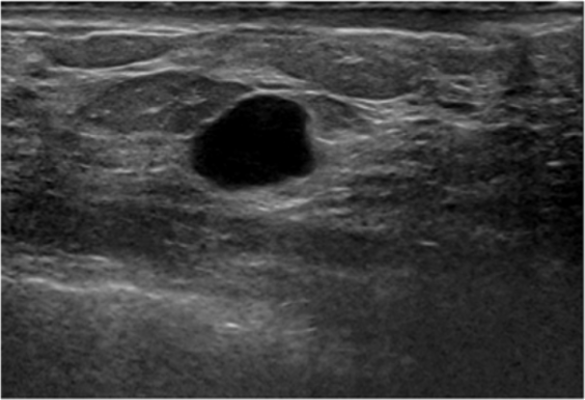
\includegraphics[width=2.6cm]{us.png}};
          \node[below=of us] (gt) {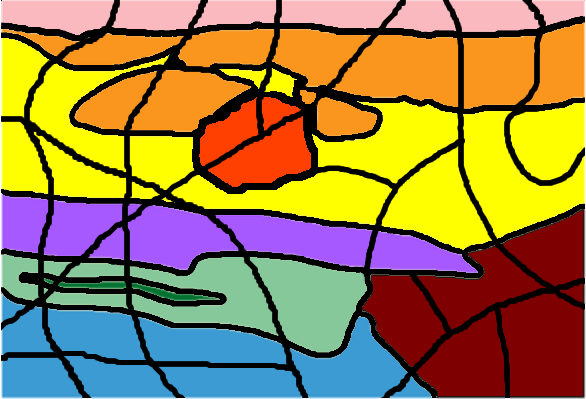
\includegraphics[width=2.6cm]{gt.png}};
        \end{tikzpicture}
        \label{fig:methodTerms:problem}
    \end{subfloat}
    %\hfill
    \begin{subfloat}
        \centering
        \begin{tikzpicture}[node distance=3pt, inner sep=0]
          \node[]           (a){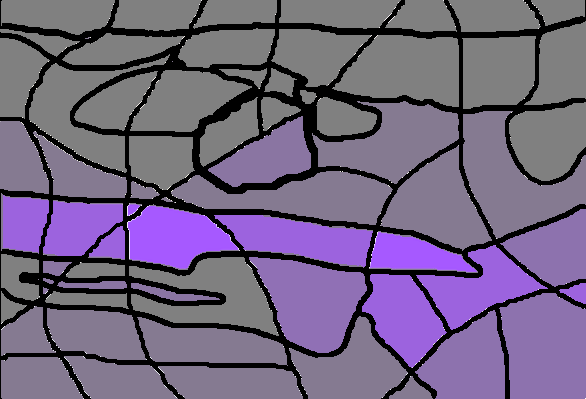
\includegraphics[width=2.6cm]{a.png}};
          \node[below=of a] (b){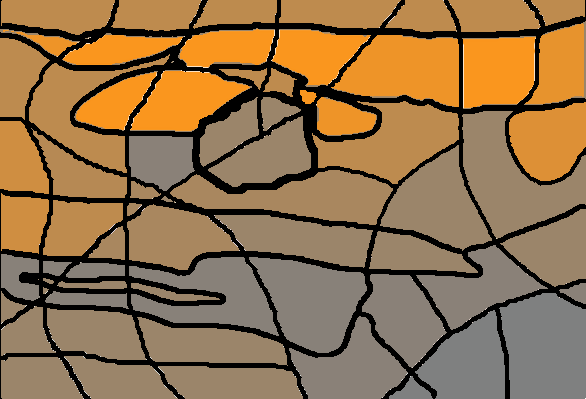
\includegraphics[width=2.6cm]{b.png}};
          \node[right=of a] (c){
\includegraphics[width=2.6cm]{c.png}};
          \node[below=of c] (d){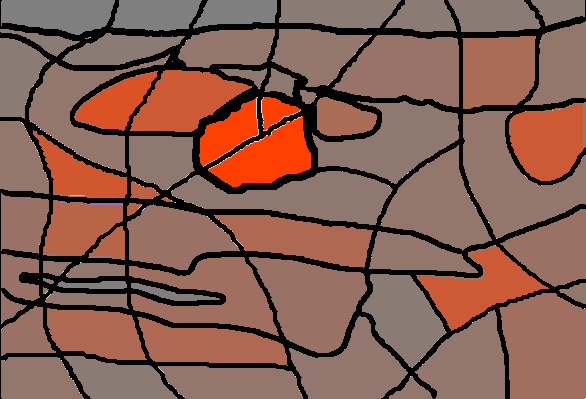
\includegraphics[width=2.6cm]{d.png}};
        \end{tikzpicture}
        \label{fig:methodTerms:data}
    \end{subfloat}
    %\hfill
    \begin{subfloat}
        \centering
        \begin{tikzpicture}[node distance=3pt, inner sep=0]
          \node[]           (a){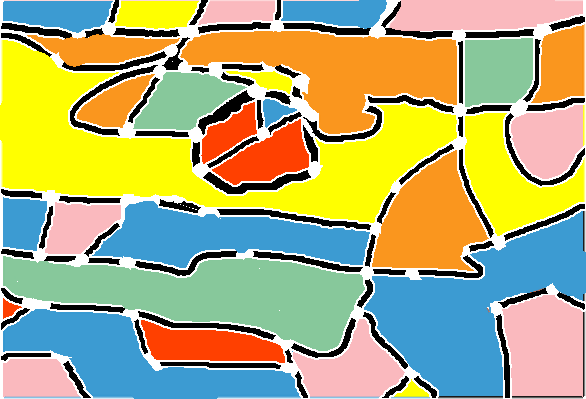
\includegraphics[width=2.6cm]{f.png}};
          \node[below=of a] (b){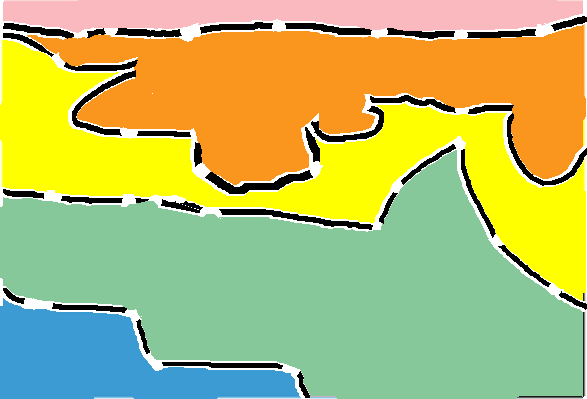
\includegraphics[width=2.6cm]{g.png}};
        \end{tikzpicture}
        %\caption[]% {{\small Pairwise term }}
        \label{fig:methodTerms:boundary}
    \end{subfloat}
    \\
    \centering
    \begin{subfloat}
        \centering
        \documentclass{standalone}
\usepackage[utf8]{inputenc}
\usepackage{tikz}
\usetikzlibrary{shapes, arrows, arrows.meta, positioning, fit, calc}
\usepackage{pgfplots,pgfplotstable}
\pgfplotsset{compat=1.8}

% % This tex, loads the Breast GT pallete if is not defined.
% The document takes advantage of the xcolor package primitive 
% \def\@ifundefinedcolor#1{\@ifundefined{\string\color@#1}}
% therefore it xcolor package is needed or the definitions needs to be added.
% 
% TODO: 
% 	create a more generic script that checks if all the packages are there otherwise loads them.
%	or defines the missing primitive.
%   take a look at: \@ifpackageloaded{<name>}{<true>}{<false>}
% 					http://tex.stackexchange.com/questions/16199/test-if-a-package-or-package-option-is-loaded

\makeatletter
\newcommand{\colorprovide}[2]{%
  \@ifundefinedcolor{#1}{\colorlet{#1}{#2}}{}}

\newcommand{\defineColorWhenNoExist}[3]{%
  \@ifundefinedcolor{#1}{\definecolor{#1}{#2}{#3}}{}}
\makeatother

\defineColorWhenNoExist{bgColor}{rgb}{0.0000, 0.0000, 0.0000}
\defineColorWhenNoExist{boundaryColor}{rgb}{0.8784, 0.8784, 0.7529}
\defineColorWhenNoExist{chestWallColor}{rgb}{0.5294, 0.7843, 0.6078}
\defineColorWhenNoExist{fatColor}{rgb}{0.9804, 0.5882, 0.1176}
\defineColorWhenNoExist{fibroGlandColor}{rgb}{1.0000, 1.0000, 0.0000}
\defineColorWhenNoExist{lesionColor}{rgb}{1.0000, 0.2510, 0.0000}
\defineColorWhenNoExist{lungColor}{rgb}{0.2353, 0.6078, 0.8235}
\defineColorWhenNoExist{pectoralColor}{rgb}{0.6510, 0.3490, 1.0000}
\defineColorWhenNoExist{ribColor}{rgb}{0.0000, 0.4510, 0.1961}
\defineColorWhenNoExist{skinColor}{rgb}{0.9804, 0.7255, 0.7451}
\defineColorWhenNoExist{unkTissueColor}{rgb}{0.6000, 0.3020, 0.2510}


\newenvironment{customlegend}[1][]{%
    \begingroup
    % inits/clears the lists (which might be populated from previous
    % axes):
    \csname pgfplots@init@cleared@structures\endcsname
    \pgfplotsset{#1}%
}{%
    % draws the legend:
    \csname pgfplots@createlegend\endcsname
    \endgroup
}%
% makes \addlegendimage available (typically only available within an
% axis environment):
\def\addlegendimage{\csname pgfplots@addlegendimage\endcsname}

\begin{document}

\makeatletter
\newcommand{\colorprovide}[2]{%
  \@ifundefinedcolor{#1}{\colorlet{#1}{#2}}{}}

\newcommand{\defineColorWhenNoExist}[3]{%
  \@ifundefinedcolor{#1}{\definecolor{#1}{#2}{#3}}{}}
\makeatother

\defineColorWhenNoExist{bgColor}{RGB}{127, 0, 0}
\defineColorWhenNoExist{boundaryColor}{rgb}{0, 0, 0}
\defineColorWhenNoExist{chestWallColor}{rgb}{0.5294, 0.7843, 0.6078}
\defineColorWhenNoExist{fatColor}{rgb}{0.9804, 0.5882, 0.1176}
\defineColorWhenNoExist{fibroGlandColor}{rgb}{1.0000, 1.0000, 0.0000}
\defineColorWhenNoExist{lesionColor}{rgb}{1.0000, 0.2510, 0.0000}
\defineColorWhenNoExist{lungColor}{rgb}{0.2353, 0.6078, 0.8235}
\defineColorWhenNoExist{pectoralColor}{rgb}{0.6510, 0.3490, 1.0000}
\defineColorWhenNoExist{ribColor}{rgb}{0.0000, 0.4510, 0.1961}
\defineColorWhenNoExist{skinColor}{rgb}{0.9804, 0.7255, 0.7451}
\defineColorWhenNoExist{unkTissueColor}{rgb}{0.6000, 0.3020, 0.2510}

\tikzstyle{myLegendStyle} = [ align=left,
                              draw=none,
                              column sep=3pt,
                              font=\tiny,
                            ]

% \begin{tikzpicture}[node distance=16pt, inner sep=0]

%   \node[](problem){
%       \begin{tikzpicture}[node distance=3pt, inner sep=0]
%         \node[]            (us) {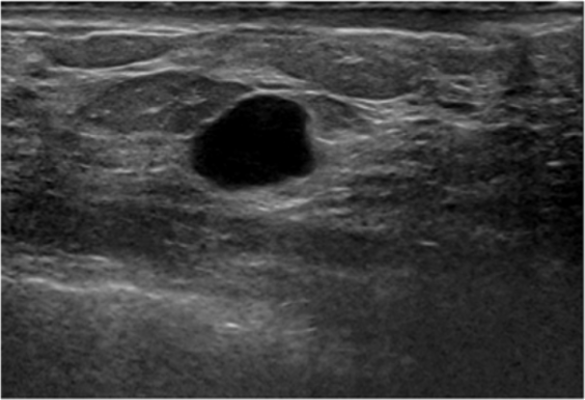
\includegraphics[]{us.png}};
%         \node[below=of us] (gt) {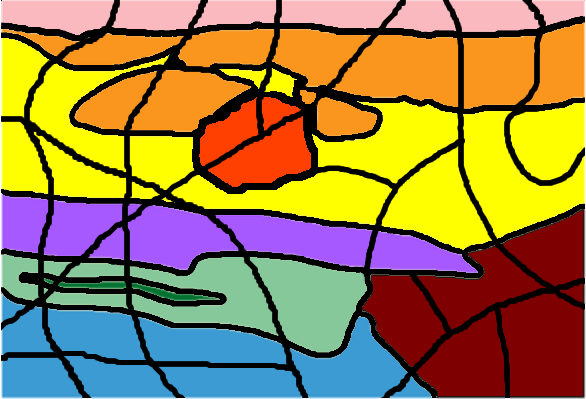
\includegraphics[]{gt.png}};
%       \end{tikzpicture}
%   };

%   \node[right=of problem](data){
%       \begin{tikzpicture}[node distance=3pt, inner sep=0]
%         \node[]           (a){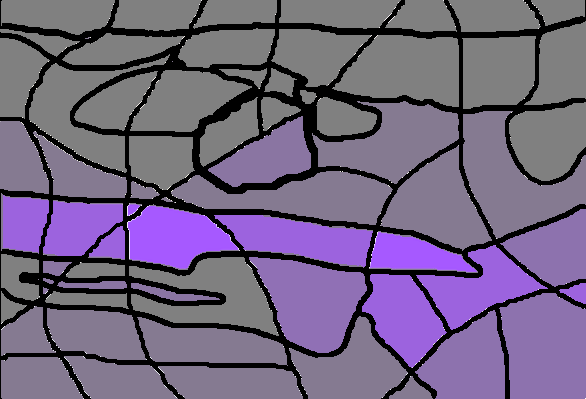
\includegraphics[]{a.png}};
%         \node[below=of a] (b){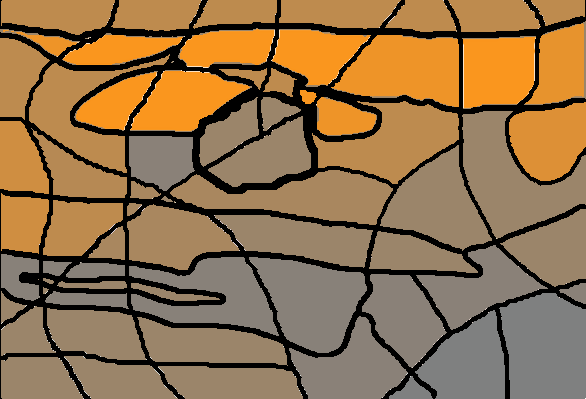
\includegraphics[]{b.png}};
%         \node[right=of a] (c){
\includegraphics[]{c.png}};
%         \node[below=of c] (d){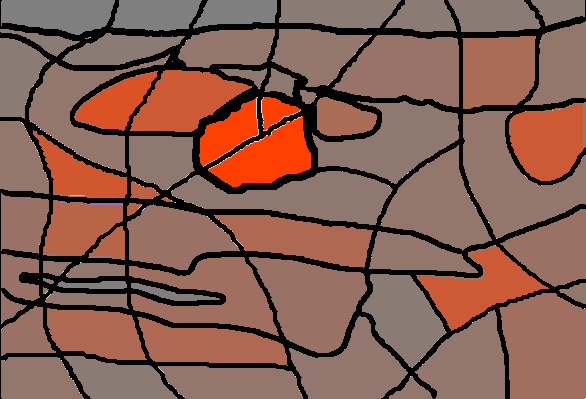
\includegraphics[]{d.png}};
%       \end{tikzpicture}
%   };

%   \node[right=of data](smooth){
%       \begin{tikzpicture}[node distance=3pt, inner sep=0]
%         \node[]           (a){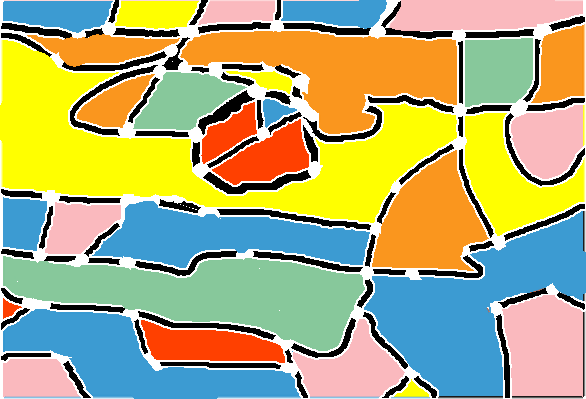
\includegraphics[]{f.png}};
%         \node[below=of a] (b){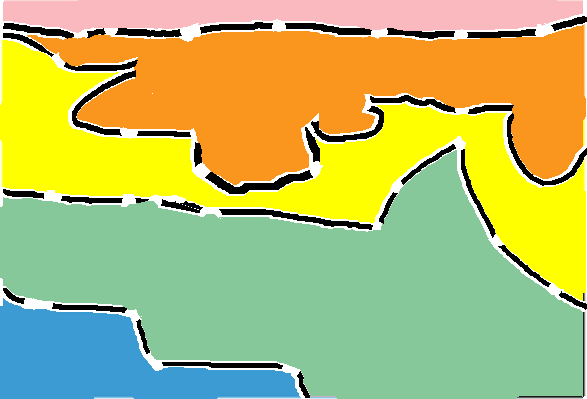
\includegraphics[]{g.png}};
%       \end{tikzpicture}
%   };

%   \node[below=of data](legend){
      \begin{tikzpicture} \begin{customlegend}
        [ legend columns=   5,
          legend style  =   myLegendStyle,
          legend entries= { Background,
            Chest wall,
            Pectoral muscle,
            Adipose tissue,
            Lesion,
            Air (or lungs),
            Rib,
            Fibro-glandular tissue,
            Skin,
            Edge,
          },
        ]

        %  \addMyLegendArea{red}
        \addlegendimage{bgColor!50!black,         fill=bgColor,         area legend}
        \addlegendimage{chestWallColor!50!black,  fill=chestWallColor,  area legend}
        \addlegendimage{pectoralColor!50!black,   fill=pectoralColor,   area legend}
        \addlegendimage{fatColor!50!black,        fill=fatColor,        area legend}
        \addlegendimage{lesionColor!50!black,     fill=lesionColor,     area legend}
        \addlegendimage{lungColor!50!black,       fill=lungColor,       area legend}
        \addlegendimage{ribColor!50!black,        fill=ribColor,        area legend}
        \addlegendimage{fibroGlandColor!50!black, fill=fibroGlandColor, area legend}
        \addlegendimage{skinColor!50!black,       fill=skinColor,       area legend}
        \addlegendimage{boundaryColor!50!black,   fill=boundaryColor,   area legend}
      \end{customlegend} \end{tikzpicture}
  % };

% \end{tikzpicture}
\end{document}



        %\caption[]% {{\small Pairwise term }}
        \label{fig:methodTerms:gt}
    \end{subfloat}

    \caption {
      \protect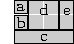
\includegraphics[height=1em]{fig_legend.pdf}
      \small Methodology Highlights.
      % \protect\tikz{\node[draw, minimum width=10pt, minimum height=10pt](0){x};}
      (a) \acs{bus} image example.
      (b) Superpixels' representation coloured using dataset's accompanying multi-label \acs{gt}.
      (c) \ac{gt} color code.
      (d) Data term: cost of labelling all sites as pectoral, lungs, adipose tissue or lesion.
      For illustration purposes, highly saturated colour indicates a low data cost - i.e., high confidence to assign the label associated with the color.
      (e) Pairwise term: labelling configurations with more boundaries produce higher pairwise term cost.}
    \label{fig:methodTerms}
\end{figure*}


Optimization methodologies offer a standardized manner to approach segmentation by minimizing an application-driven cost function~\cite{cremers2007review}.
Figure~\ref{fig:method} illustrates a generic representation of the segmentation strategy,
concrete examples of its terms, applied to \ac{bus}, can be found in \cref{sec:methodApp}.
The overall segmentation can be seen as a three-steps strategy:
(1) a mapping of the image into a discrete set of elements $\mathcal{S}$,
(2) the optimization stage which is formulated as a \emph{metric labelling} problem,
and (3) a re-mapping the labels obtained from the previous stage to produce the final delineation.

\newcommand{\classificableSample}{
  \path[fill=ccccccc] (437.2282,117.5035) .. controls (421.0914,117.5542) and
    (412.9722,117.5952) .. (388.810,117.9001) .. controls (388.8066,117.9021) and
    (388.7938,117.9021) .. (388.7814,117.9008) .. controls (388.7659,117.8928) and
    (388.7528,117.8828) .. (388.7432,117.8702) .. controls (388.7277,117.8623) and
    (388.7146,117.8522) .. (388.7051,117.8397) .. controls (388.7031,117.8294) and
    (388.7031,117.8188) .. (388.7045,117.8085) -- (388.2860,115.4466) .. controls
    (388.2840,115.4363) and (388.2840,115.4257) .. (388.2854,115.4154) .. controls
    (388.2954,115.4025) and (388.3073,115.3915) .. (388.3224,115.3835) .. controls
    (402.8137,115.1621) and (420.6557,115.1538) .. (434.4327,115.1976) .. controls
    (439.1681,115.0982) and (444.4764,115.4449) .. (448.1281,115.0823) --
    (448.3173,117.5246) .. controls (445.7548,117.6739) and (440.9246,117.4918) ..
    (437.2282,117.5035) -- cycle;
  \path[fill=ccccccc] (437.2282,111.6456) .. controls (421.0913,111.6963) and
    (412.9722,111.7373) .. (388.8190,112.0422) .. controls (388.8066,112.0442) and
    (388.7938,112.0442) .. (388.7814,112.0429) .. controls (388.7659,112.0349) and
    (388.7528,112.0249) .. (388.7432,112.0124) .. controls (388.7277,112.0044) and
    (388.7146,111.9944) .. (388.7051,111.9819) .. controls (388.7031,111.9716) and
    (388.7031,111.9610) .. (388.7045,111.9507) -- (388.2860,109.5888) .. controls
    (388.2840,109.5785) and (388.2840,109.5679) .. (388.2854,109.5576) .. controls
    (388.2954,109.5447) and (388.3073,109.5337) .. (388.3224,109.5257) .. controls
    (402.8137,109.3042) and (420.6557,109.2960) .. (434.4327,109.3398) .. controls
    (439.1680,109.2404) and (444.4764,109.5870) .. (448.1281,109.2244) --
    (448.3173,111.6667) .. controls (445.7548,111.8161) and (440.9246,111.6339) ..
    (437.2282,111.6456) -- cycle;
  \path[fill=ccccccc] (437.2282,152.6507) .. controls (421.0914,152.7014) and
    (412.9722,152.7424) .. (388.8190,153.0473) .. controls (388.8066,153.0493) and
    (388.7938,153.0493) .. (388.7814,153.0480) .. controls (388.7659,153.0400) and
    (388.7528,153.0300) .. (388.7432,153.0175) .. controls (388.7277,153.0095) and
    (388.7146,152.9995) .. (388.7051,152.9870) .. controls (388.7031,152.9767) and
    (388.7031,152.9661) .. (388.7045,152.9558) -- (388.2860,150.5938) .. controls
    (388.2840,150.5835) and (388.2840,150.5729) .. (388.2854,150.5626) .. controls
    (388.2954,150.5497) and (388.3073,150.5387) .. (388.3224,150.5307) .. controls
    (402.8137,150.3093) and (420.6557,150.3010) .. (434.4327,150.3448) .. controls
    (439.1681,150.2454) and (444.4764,150.5921) .. (448.1281,150.2295) --
    (448.3173,152.6718) .. controls (445.7548,152.8211) and (440.9246,152.6390) ..
    (437.2282,152.6507) -- cycle;
  \path[fill=ccccccc] (437.2282,135.0770) .. controls (421.0914,135.1277) and
    (412.9722,135.1687) .. (388.8190,135.4737) .. controls (388.8066,135.4757) and
    (388.7938,135.4757) .. (388.7814,135.4743) .. controls (388.7659,135.4663) and
    (388.7528,135.4563) .. (388.7432,135.4438) .. controls (388.7277,135.4358) and
    (388.7146,135.4258) .. (388.7051,135.4133) .. controls (388.7031,135.4030) and
    (388.7031,135.3924) .. (388.7045,135.3821) -- (388.2860,133.0202) .. controls
    (388.2840,133.0099) and (388.2840,132.9993) .. (388.2854,132.9890) .. controls
    (388.2954,132.9761) and (388.3073,132.9651) .. (388.3224,132.9571) .. controls
    (402.8137,132.7357) and (420.6557,132.7274) .. (434.4327,132.7712) .. controls
    (439.1681,132.6718) and (444.4764,133.0185) .. (448.1281,132.6559) --
    (448.3173,135.0982) .. controls (445.7548,135.2475) and (440.9246,135.0654) ..
    (437.2282,135.0771) -- cycle;
  \path[fill=ccccccc] (437.2282,146.7928) .. controls (421.0913,146.8435) and
    (412.9722,146.8845) .. (388.8190,147.1894) .. controls (388.8066,147.1914) and
    (388.7938,147.1914) .. (388.7814,147.1901) .. controls (388.7659,147.1821) and
    (388.7528,147.1721) .. (388.7432,147.1596) .. controls (388.7277,147.1516) and
    (388.7146,147.1416) .. (388.7051,147.1291) .. controls (388.7031,147.1188) and
    (388.7031,147.1082) .. (388.7045,147.0979) -- (388.2860,144.7360) .. controls
    (388.2840,144.7257) and (388.2840,144.7151) .. (388.2854,144.7048) .. controls
    (388.2954,144.6919) and (388.3073,144.6809) .. (388.3224,144.6729) .. controls
    (402.8137,144.4514) and (420.6557,144.4431) .. (434.4327,144.4870) .. controls
    (439.1680,144.3876) and (444.4764,144.7342) .. (448.1281,144.3716) --
    (448.3173,146.8139) .. controls (445.7548,146.9633) and (440.9246,146.7811) ..
    (437.2282,146.7928) -- cycle;
  \path[fill=ccccccc] (388.8145,122.5780) -- (388.8145,121.0897) --
    (391.9611,121.0033) .. controls (396.7480,120.8718) and (426.4910,120.6312) ..
    (437.7817,120.6327) -- (447.7872,120.6347) -- (447.7872,122.1722) --
    (447.7872,123.7096) -- (446.1255,123.7985) .. controls (445.2116,123.8474) and
    (433.6133,123.8804) .. (420.3515,123.8719) .. controls (407.0897,123.8629) and
    (394.5686,123.9038) .. (392.5268,123.9616) -- (388.8145,124.0670) --
    (388.8145,122.5787) -- cycle;
  \path[fill=ccccccc] (388.8146,140.1454) -- (388.8146,138.7157) --
    (393.9411,138.6220) .. controls (402.5246,138.4652) and (435.0187,138.2305) ..
    (441.5997,138.2779) -- (447.7866,138.3225) -- (447.7869,139.8296) --
    (447.7872,141.3367) -- (446.4790,141.4209) .. controls (445.7595,141.4672) and
    (432.4907,141.5209) .. (416.9926,141.5401) -- (388.8146,141.5751) --
    (388.8146,140.1454) -- cycle;
  \path[fill=ccccccc] (388.8145,128.3965) -- (388.8145,126.9648) --
    (395.9916,126.8645) .. controls (408.6691,126.6873) and (436.9417,126.5307) ..
    (442.4486,126.6071) -- (447.7872,126.6812) -- (447.7872,128.1347) --
    (447.7872,129.5881) -- (446.9033,129.6680) .. controls (446.4172,129.7119) and
    (433.1483,129.7660) .. (417.4170,129.7880) -- (388.8145,129.8281) --
    (388.8145,128.3965) -- cycle;
  \path[draw=black, line join=round,miter limit=4.00,rounded
    corners=0.0000cm] (388.3896,107.8040) rectangle (448.1925,152.8885);
  \path[draw=black, very thin, line join=miter,line cap=butt]
    (437.6521,107.9420) -- (437.3693,153.1969);
  \path[draw=black, very thin, line join=miter,line cap=butt]
    (432.0895,107.9420) -- (431.8067,153.1969);
  \path[draw=black, very thin, line join=miter,line cap=butt]
    (426.5269,107.9420) -- (426.2441,153.1969);
  \path[draw=black, very thin, line join=miter,line cap=butt]
    (420.9643,107.9420) -- (420.6815,153.1969);
  \path[draw=black, very thin, line join=miter,line cap=butt]
    (415.4017,107.9420) -- (415.1189,153.1969);
  \path[draw=black, very thin, line join=miter,line cap=butt]
    (409.8391,107.9420) -- (409.5563,153.1969);
  \path[draw=black, very thin, line join=miter,line cap=butt]
    (404.2765,107.9420) -- (403.9937,153.1969);
  \path[draw=black, very thin, line join=miter,line cap=butt]
    (398.7140,107.9420) -- (398.4311,153.1969);
  \path[draw=black, very thin, line join=miter,line cap=butt]
    (393.1513,108.2249) -- (392.8685,153.4797);
  \path[draw=black, very thin, line join=miter,line cap=butt]
    (443.2147,107.6592) -- (442.9319,152.9140);


}

\newcommand{\rigitMapping}{
  \path[draw=black] (263.4135,303.2951) -- (293.2817,303.9377)
    -- (294.2726,328.7912) -- (262.8174,328.8772) -- (263.4135,303.2952) -- cycle;
  \path[draw=black] (263.4135, 307.1946) -- (293.2817, 307.8371);
  \path[draw=black] (290.5946, 303.8316) -- (291.5855, 328.8266);
  \path[draw=black] (293.9190, 320.6790) -- (262.8174, 320.9064);
  \path[draw=black] (286.3273, 328.8418) -- (286.9941, 303.8608);
  \path[draw=black] (278.7718, 303.2952) -- (278.7718, 303.2951);
  \path[draw=black] (276.1752, 329.0186) -- (276.7714, 303.4366);
  \path[draw=black] (266.4943, 328.8772) -- (267.0905, 303.2952);
  \path[draw=black] (281.6652, 303.7962) -- (282.6561, 328.6498);
  \path[draw=black] (270.5495, 303.2305) -- (271.6819, 328.8973);
  \path[draw=black] (263.4135, 311.7365) -- (293.5645, 312.2376);
  \path[draw=black] (263.4135, 316.2785) -- (293.7766, 315.9310);
  \path[draw=black] (294.2726, 324.8058) -- (262.8174, 324.8918);
  \path[draw=black] (294.2726, 328.7912) -- (262.8174, 328.8772);
}

\newcommand{\pointMapping}{
  \path[fill=black] (357.4620,315.8718) .. controls (356.1805,316.0253) and
    (358.2131,317.4454) .. (357.8163,316.1789) -- (357.6510,316.0135) --
    (357.4620,315.8718) -- cycle;
  \path[fill=black] (355.3124,315.9190) .. controls (354.3296,316.0308) and
    (355.3729,317.9314) .. (355.9975,316.7221) .. controls (356.1310,316.3826) and
    (355.9457,315.8904) .. (355.5250,315.9190) .. controls (355.4406,315.9090) and
    (355.3780,315.9120) .. (355.3124,315.9190) -- cycle;
  \path[fill=black] (359.8242,315.9190) .. controls (358.1549,316.1517) and
    (360.6806,318.1230) .. (360.6273,316.3915) .. controls (360.5177,316.0706) and
    (360.1595,315.8345) .. (359.8242,315.9190) -- cycle;
  \path[fill=black] (366.8162,315.9190) .. controls (366.3028,315.9764) and
    (365.6288,317.0045) .. (366.6744,317.2182) .. controls (367.0123,317.2905) and
    (367.2590,316.9059) .. (367.2414,316.6040) .. controls (367.2514,316.0656) and
    (367.0495,315.8929) .. (366.8162,315.9190) -- cycle;
  \path[fill=black] (361.7848,315.9662) .. controls (360.8648,315.9556) and
    (361.8595,317.7951) .. (362.3517,316.6040) .. controls (362.5026,316.3316) and
    (362.3350,315.9275) .. (361.9974,315.9898) .. controls (361.9183,315.9713) and
    (361.8461,315.9669) .. (361.7848,315.9662) -- cycle;
  \path[fill=black] (352.9503,315.9898) .. controls (351.4262,315.9808) and
    (353.4582,318.1125) .. (353.4936,316.4386) .. controls (353.4413,316.1883) and
    (353.2231,315.9534) .. (352.9503,315.9898) -- cycle;
  \path[fill=black] (345.9819,316.0134) .. controls (344.7004,316.1669) and
    (346.7093,317.5870) .. (346.3126,316.3205) -- (346.1472,316.1315) --
    (345.9819,316.0134) -- cycle;
  \path[fill=black] (364.0288,316.0134) .. controls (362.3104,316.3211) and
    (364.5570,318.7762) .. (364.7375,316.8165) .. controls (364.7483,316.4176) and
    (364.4507,316.0013) .. (364.0288,316.0134) -- cycle;
  \path[fill=black] (367.8791,316.0134) .. controls (367.7217,316.0140) and
    (367.5694,316.1352) .. (367.5721,316.2969) .. controls (367.6362,318.0646) and
    (369.6502,316.3318) .. (367.8791,316.0134) -- cycle;
  \path[fill=black] (343.8087,316.0606) .. controls (342.8258,316.1724) and
    (343.8928,318.0730) .. (344.5174,316.8637) .. controls (344.6510,316.5242) and
    (344.4656,316.0320) .. (344.0449,316.0606) .. controls (343.9605,316.0506) and
    (343.8742,316.0536) .. (343.8087,316.0606) -- cycle;
  \path[fill=black] (348.3441,316.0606) .. controls (346.6748,316.2933) and
    (349.1769,318.2409) .. (349.1236,316.5094) .. controls (349.0140,316.1885) and
    (348.6794,315.9761) .. (348.3441,316.0606) -- cycle;
  \path[fill=black] (350.3046,316.1078) .. controls (349.3847,316.0972) and
    (350.3793,317.9131) .. (350.8716,316.7220) .. controls (351.0225,316.4495) and
    (350.8549,316.0691) .. (350.5172,316.1314) .. controls (350.4382,316.1129) and
    (350.3660,316.1085) .. (350.3046,316.1078) -- cycle;
  \path[fill=black] (339.6041,316.1550) .. controls (337.8364,316.4703) and
    (339.8402,318.2047) .. (339.9111,316.4385) .. controls (339.9131,316.2768) and
    (339.7617,316.1569) .. (339.6041,316.1550) -- cycle;
  \path[fill=black] (341.2812,316.2022) .. controls (341.2384,316.1972) and
    (341.1878,316.2164) .. (341.1395,316.2258) .. controls (339.6970,316.4281) and
    (341.5078,318.4878) .. (341.7064,316.9108) .. controls (341.7325,316.6269) and
    (341.5809,316.2394) .. (341.2812,316.2022) -- cycle;
  \path[fill=black] (366.6508,317.5723) .. controls (366.5103,317.5720) and
    (366.2950,317.6796) .. (366.0130,317.9738) -- (365.9658,318.1628) --
    (365.9658,318.3754) .. controls (366.6561,319.6892) and (367.2598,317.5734) ..
    (366.6509,317.5723) -- cycle;
  \path[fill=black] (368.0209,317.5723) .. controls (367.7357,317.6540) and
    (367.4955,317.8821) .. (367.4067,318.1628) .. controls (367.4097,319.7890) and
    (369.7206,317.5939) .. (368.0209,317.5723) -- cycle;
  \path[fill=black] (339.6277,317.8085) .. controls (339.5551,317.8045) and
    (339.4688,317.8190) .. (339.3678,317.8321) .. controls (339.1248,317.9408) and
    (338.9287,318.1364) .. (338.7773,318.3518) .. controls (338.7733,319.7430) and
    (340.7160,317.8729) .. (339.6277,317.8085) -- cycle;
  \path[fill=black] (357.5801,317.9738) .. controls (356.0712,318.0409) and
    (358.0502,320.0753) .. (358.1470,318.4463) .. controls (358.1359,318.1690) and
    (357.8786,317.8529) .. (357.5801,317.9738) -- cycle;
  \path[fill=black] (355.1235,318.0211) .. controls (353.4135,317.9960) and
    (355.1757,320.5675) .. (355.5723,318.7062) .. controls (355.6234,318.4095) and
    (355.4571,318.0563) .. (355.1235,318.0211) -- cycle;
  \path[fill=black] (346.3126,318.0920) .. controls (346.2464,318.0768) and
    (346.1746,318.0850) .. (346.1000,318.1156) .. controls (344.5911,318.1826) and
    (346.5465,320.1935) .. (346.6433,318.5644) .. controls (346.6353,318.3565) and
    (346.5111,318.1376) .. (346.3126,318.0920) -- cycle;
  \path[fill=black] (343.6434,318.1393) .. controls (341.9334,318.1142) and
    (343.6720,320.7093) .. (344.0685,318.8480) .. controls (344.1196,318.5513) and
    (343.9770,318.1744) .. (343.6434,318.1393) -- cycle;
  \path[fill=black] (362.0918,318.1629) .. controls (361.0812,318.2168) and
    (361.8505,320.2037) .. (362.4462,318.8007) .. controls (362.5193,318.5919) and
    (362.4919,318.3265) .. (362.3281,318.1629) .. controls (362.2445,318.1476) and
    (362.1592,318.1589) .. (362.0918,318.1629) -- cycle;
  \path[fill=black] (359.5879,318.1865) .. controls (357.8995,318.3351) and
    (360.0226,320.6520) .. (360.1076,318.7771) .. controls (360.1026,318.4837) and
    (359.9115,318.1719) .. (359.5879,318.1865) -- cycle;
  \path[fill=black] (363.8871,318.2574) .. controls (362.4808,318.9475) and
    (365.3454,320.1242) .. (364.5957,318.5645) .. controls (364.3912,318.4028) and
    (364.1545,318.2670) .. (363.8871,318.2574) -- cycle;
  \path[fill=black] (350.6117,318.2810) .. controls (349.6011,318.3349) and
    (350.3467,320.3454) .. (350.9424,318.9424) .. controls (351.0155,318.7336) and
    (351.0117,318.4682) .. (350.8479,318.3046) .. controls (350.7643,318.2893) and
    (350.6791,318.2774) .. (350.6117,318.2810) -- cycle;
  \path[fill=black] (348.0842,318.3046) .. controls (346.3958,318.4532) and
    (348.5425,320.7937) .. (348.6275,318.9188) .. controls (348.6225,318.6254) and
    (348.4078,318.2900) .. (348.0842,318.3046) -- cycle;
  \path[fill=black] (352.4070,318.3991) .. controls (351.0006,319.0892) and
    (353.8653,320.2659) .. (353.1156,318.7062) .. controls (352.9111,318.5445) and
    (352.6744,318.4087) .. (352.4070,318.3991) -- cycle;
  \path[fill=black] (340.8088,318.4464) .. controls (339.6929,319.3698) and
    (342.2285,320.1726) .. (341.7064,318.8480) .. controls (341.4655,318.6196) and
    (341.1356,318.4835) .. (340.8088,318.4464) -- cycle;
  \path[fill=black] (367.7610,319.7456) .. controls (367.5543,319.8006) and
    (367.4007,320.0154) .. (367.4067,320.2417) .. controls (367.4680,321.8317) and
    (369.5431,320.3602) .. (367.9973,319.7456) .. controls (367.9234,319.7283) and
    (367.8300,319.7273) .. (367.7610,319.7456) -- cycle;
  \path[fill=black] (366.6508,319.8874) .. controls (366.5208,319.8844) and
    (366.3837,319.9450) .. (366.2965,320.0055) .. controls (365.1993,320.5281) and
    (367.0803,321.2192) .. (366.9107,320.1000) .. controls (366.8912,319.9422) and
    (366.7809,319.8902) .. (366.6508,319.8874) -- cycle;
  \path[fill=black] (339.4151,320.0527) .. controls (337.8132,320.4022) and
    (339.9137,321.8549) .. (340.0056,320.4543) .. controls (339.9662,320.1806) and
    (339.6762,320.0265) .. (339.4151,320.0527) -- cycle;
  \path[fill=black] (355.0762,320.2417) .. controls (354.8150,320.2307) and
    (354.5585,320.4452) .. (354.5093,321.0448) .. controls (354.5073,321.3008) and
    (354.7205,321.5398) .. (354.9817,321.5645) .. controls (356.2956,321.3384) and
    (355.6510,320.2659) .. (355.0762,320.2417) -- cycle;
  \path[fill=black] (357.4856,320.2417) .. controls (356.9401,320.2427) and
    (356.2898,321.0171) .. (357.3911,321.2574) .. controls (357.6523,321.2836) and
    (357.9423,321.1059) .. (357.9817,320.8322) .. controls (357.9530,320.3945) and
    (357.7336,320.2410) .. (357.4856,320.2417) -- cycle;
  \path[fill=black] (343.5961,320.3834) .. controls (343.3349,320.3724) and
    (343.0784,320.5633) .. (343.0292,321.1629) .. controls (343.0272,321.4189) and
    (343.2168,321.6816) .. (343.4780,321.7062) .. controls (344.7919,321.4801) and
    (344.1709,320.4076) .. (343.5961,320.3834) -- cycle;
  \path[fill=black] (345.9819,320.3834) .. controls (345.4363,320.3844) and
    (344.7861,321.1588) .. (345.8874,321.3991) .. controls (346.1486,321.4254) and
    (346.4385,321.2476) .. (346.4779,320.9739) .. controls (346.4492,320.5363) and
    (346.2299,320.3828) .. (345.9819,320.3834) -- cycle;
  \path[fill=black] (364.2887,320.5015) .. controls (363.8717,320.4808) and
    (363.3903,320.8835) .. (364.0761,321.2102) .. controls (364.2504,321.3312) and
    (364.6749,321.4076) .. (364.7138,321.0920) .. controls (364.7774,320.6723) and
    (364.5388,320.5139) .. (364.2887,320.5015) -- cycle;
  \path[fill=black] (362.0210,320.5487) .. controls (361.5794,320.5375) and
    (361.1433,320.9401) .. (361.9738,321.2337) .. controls (362.1488,321.3150) and
    (362.4857,321.4245) .. (362.5407,321.1392) .. controls (362.5387,320.7087) and
    (362.2860,320.5554) .. (362.0210,320.5487) -- cycle;
  \path[fill=black] (360.0368,320.5959) .. controls (359.5427,320.6350) and
    (359.0090,321.1412) .. (359.8242,321.4699) .. controls (360.0942,321.5727) and
    (360.5326,321.5115) .. (360.6037,321.1865) .. controls (360.6305,320.7260) and
    (360.3332,320.5725) .. (360.0368,320.5959) -- cycle;
  \path[fill=black] (352.8086,320.6432) .. controls (352.3916,320.6225) and
    (351.9102,321.0016) .. (352.5960,321.3282) .. controls (352.7703,321.4493) and
    (353.1712,321.5493) .. (353.2101,321.2337) .. controls (353.2737,320.8140) and
    (353.0587,320.6556) .. (352.8086,320.6432) -- cycle;
  \path[fill=black] (350.5172,320.6668) .. controls (350.0757,320.6556) and
    (349.6395,321.0818) .. (350.4701,321.3755) .. controls (350.6451,321.4568) and
    (351.0056,321.5662) .. (351.0606,321.2810) .. controls (351.0586,320.8504) and
    (350.7822,320.6735) .. (350.5173,320.6668) -- cycle;
  \path[fill=black] (341.3521,320.7377) .. controls (341.2178,320.7960) and
    (341.0809,320.8740) .. (340.9741,320.9739) .. controls (340.1710,322.4980) and
    (342.9088,320.7115) .. (341.3521,320.7377) -- cycle;
  \path[fill=black] (348.5566,320.7377) .. controls (348.0626,320.7768) and
    (347.5288,321.2830) .. (348.3441,321.6117) .. controls (348.6141,321.7145) and
    (349.0289,321.6296) .. (349.1000,321.3046) .. controls (349.1267,320.8442) and
    (348.8531,320.7143) .. (348.5567,320.7377) -- cycle;
  \path[fill=black] (366.6508,321.1629) .. controls (366.5103,321.1626) and
    (366.2950,321.2702) .. (366.0130,321.5645) -- (365.9658,321.7771) --
    (365.9658,321.9897) .. controls (366.6561,323.3035) and (367.2598,321.1640) ..
    (366.6509,321.1629) -- cycle;
  \path[fill=black] (368.0209,321.1865) .. controls (367.7357,321.2682) and
    (367.4955,321.4964) .. (367.4067,321.7771) .. controls (367.4097,323.4032) and
    (369.7206,321.2082) .. (368.0209,321.1865) -- cycle;
  \path[fill=black] (339.6277,321.4227) .. controls (339.5551,321.4187) and
    (339.4688,321.4332) .. (339.3678,321.4463) .. controls (339.1248,321.5550) and
    (338.9287,321.7271) .. (338.7773,321.9424) .. controls (338.7733,323.3336) and
    (340.7160,321.4872) .. (339.6277,321.4227) -- cycle;
  \path[fill=black] (354.8872,322.4384) .. controls (354.6814,322.4622) and
    (354.5328,322.6618) .. (354.5329,323.0999) .. controls (354.6294,323.4047) and
    (354.8610,323.6489) .. (355.1707,323.7376) .. controls (356.5569,323.7123) and
    (355.5047,322.3672) .. (354.8873,322.4384) -- cycle;
  \path[fill=black] (357.0841,322.4384) .. controls (356.9027,322.4434) and
    (356.7524,322.5871) .. (356.7534,322.9581) .. controls (356.9048,323.1734) and
    (357.1008,323.3691) .. (357.3439,323.4778) .. controls (358.5555,323.6352) and
    (357.6282,322.4242) .. (357.0841,322.4384) -- cycle;
  \path[fill=black] (364.0761,322.4857) .. controls (363.9405,322.5190) and
    (363.8152,322.6573) .. (363.7217,322.9581) .. controls (363.6730,323.2513) and
    (363.7929,323.5790) .. (364.0524,323.7376) .. controls (365.3929,324.2051) and
    (364.6637,322.3414) .. (364.0760,322.4857) -- cycle;
  \path[fill=black] (362.2572,322.5566) .. controls (362.1845,322.5525) and
    (362.0985,322.5672) .. (361.9974,322.5802) .. controls (361.7540,322.6886) and
    (361.5572,322.8835) .. (361.4068,323.0998) .. controls (361.4028,324.4936) and
    (363.3476,322.6222) .. (362.2572,322.5565) -- cycle;
  \path[fill=black] (343.4071,322.5802) .. controls (343.2013,322.6039) and
    (343.0291,322.7798) .. (343.0292,323.2179) .. controls (343.1257,323.5228) and
    (343.3809,323.7906) .. (343.6906,323.8793) .. controls (345.0768,323.8540) and
    (344.0246,322.5089) .. (343.4071,322.5802) -- cycle;
  \path[fill=black] (345.5803,322.5802) .. controls (345.3990,322.5851) and
    (345.2723,322.7288) .. (345.2733,323.0998) .. controls (345.4247,323.3151) and
    (345.6207,323.5108) .. (345.8638,323.6195) .. controls (347.0754,323.7769) and
    (346.1244,322.5659) .. (345.5803,322.5802) -- cycle;
  \path[fill=black] (359.8714,322.5802) .. controls (359.7440,322.6053) and
    (359.6101,322.7206) .. (359.4698,322.9345) .. controls (359.2176,323.1228) and
    (359.2472,323.6544) .. (359.6352,323.6195) .. controls (360.7188,323.7880) and
    (360.4236,322.4708) .. (359.8714,322.5802) -- cycle;
  \path[fill=black] (352.5960,322.6037) .. controls (352.4604,322.6370) and
    (352.3351,322.7990) .. (352.2416,323.0998) .. controls (352.1929,323.3930) and
    (352.3128,323.7208) .. (352.5723,323.8793) .. controls (353.9128,324.3468) and
    (353.1835,322.4595) .. (352.5959,322.6037) -- cycle;
  \path[fill=black] (350.7535,322.6982) .. controls (350.6808,322.6942) and
    (350.5948,322.7088) .. (350.4936,322.7218) .. controls (350.2502,322.8303) and
    (350.0534,323.0016) .. (349.9031,323.2179) .. controls (349.8991,324.6117) and
    (351.8439,322.7639) .. (350.7535,322.6982) -- cycle;
  \path[fill=black] (348.3913,322.7219) .. controls (348.2639,322.7471) and
    (348.1064,322.8387) .. (347.9661,323.0525) .. controls (347.7139,323.2409) and
    (347.7671,323.7961) .. (348.1551,323.7612) .. controls (349.2387,323.9297) and
    (348.9435,322.6125) .. (348.3913,322.7218) -- cycle;
  \path[fill=black] (341.2103,322.8872) .. controls (341.0698,322.8832) and
    (340.9472,323.0027) .. (340.9505,323.3596) .. controls (341.0408,323.5085) and
    (341.1403,323.6542) .. (341.2812,323.7612) .. controls (342.3468,324.0798) and
    (341.6320,322.8985) .. (341.2103,322.8872) -- cycle;
  \path[fill=black] (367.7610,323.3596) .. controls (367.5543,323.4146) and
    (367.4007,323.6058) .. (367.4067,323.8321) .. controls (367.4680,325.4221) and
    (369.5431,323.9742) .. (367.9973,323.3596) .. controls (367.9234,323.3423) and
    (367.8300,323.3413) .. (367.7610,323.3596) -- cycle;
  \path[fill=black] (366.6508,323.5014) .. controls (366.5208,323.4984) and
    (366.3837,323.5354) .. (366.2965,323.5959) .. controls (365.1993,324.1185) and
    (367.0803,324.8332) .. (366.9107,323.7140) .. controls (366.8912,323.5562) and
    (366.7809,323.5042) .. (366.6508,323.5014) -- cycle;
  \path[fill=black] (339.4151,323.6431) .. controls (337.8132,323.9926) and
    (339.9137,325.4689) .. (340.0056,324.0683) .. controls (339.9662,323.7946) and
    (339.6762,323.6169) .. (339.4151,323.6431) -- cycle;
  \path[fill=black] (364.4776,324.5643) .. controls (362.9566,324.8751) and
    (365.0762,326.9016) .. (365.0445,325.1785) .. controls (365.0622,324.8767) and
    (364.8155,324.4921) .. (364.4776,324.5643) -- cycle;
  \path[fill=black] (357.4148,324.6588) .. controls (356.9197,324.6230) and
    (356.3648,325.5287) .. (357.5801,325.7454) .. controls (357.7378,325.7434) and
    (357.8887,325.6000) .. (357.8872,325.4384) .. controls (357.8650,324.8864) and
    (357.6398,324.6751) .. (357.4148,324.6588) -- cycle;
  \path[fill=black] (359.3517,324.6824) .. controls (359.1637,324.7000) and
    (358.9950,324.8703) .. (358.9029,325.2966) .. controls (358.7240,325.5056) and
    (358.8462,325.8201) .. (359.1155,325.8399) .. controls (360.5536,325.9538) and
    (359.9158,324.6296) .. (359.3517,324.6824) -- cycle;
  \path[fill=black] (352.9739,324.7060) .. controls (351.4529,325.0168) and
    (353.5724,327.0433) .. (353.5408,325.3202) .. controls (353.5585,325.0184) and
    (353.3117,324.6338) .. (352.9739,324.7060) -- cycle;
  \path[fill=black] (354.9109,324.7532) .. controls (354.6857,324.7699) and
    (354.4584,324.9803) .. (354.4384,325.5328) .. controls (354.4354,325.6944) and
    (354.5881,325.8392) .. (354.7455,325.8398) .. controls (355.9631,325.6209) and
    (355.4063,324.7164) .. (354.9109,324.7532) -- cycle;
  \path[fill=black] (362.3989,324.7768) .. controls (361.8250,324.7556) and
    (361.0485,325.3646) .. (362.1391,325.7453) .. controls (362.3032,325.9570) and
    (362.6535,325.9332) .. (362.7769,325.6980) .. controls (363.0062,325.0308) and
    (362.7433,324.7895) .. (362.3989,324.7768) -- cycle;
  \path[fill=black] (345.7929,324.8004) .. controls (345.3451,324.9097) and
    (344.9716,325.6664) .. (346.0764,325.8634) .. controls (346.2340,325.8614) and
    (346.3850,325.7416) .. (346.3835,325.5800) .. controls (346.3569,324.9176) and
    (346.0616,324.7349) .. (345.7929,324.8004) -- cycle;
  \path[fill=black] (347.8716,324.8240) .. controls (347.6836,324.8416) and
    (347.4912,325.0119) .. (347.3992,325.4382) .. controls (347.2202,325.6472) and
    (347.3661,325.9617) .. (347.6354,325.9815) .. controls (349.0735,326.0954) and
    (348.4357,324.7712) .. (347.8716,324.8240) -- cycle;
  \path[fill=black] (343.4071,324.8949) .. controls (343.1820,324.9116) and
    (342.9784,325.1220) .. (342.9583,325.6745) .. controls (342.9553,325.8361) and
    (343.1080,325.9809) .. (343.2654,325.9815) .. controls (344.4830,325.7626) and
    (343.9025,324.8581) .. (343.4071,324.8949) -- cycle;
  \path[fill=black] (350.8952,324.9185) .. controls (350.3213,324.8973) and
    (349.5684,325.5063) .. (350.6590,325.8870) .. controls (350.8231,326.0987) and
    (351.1734,326.0749) .. (351.2968,325.8397) .. controls (351.5261,325.1725) and
    (351.2396,324.9312) .. (350.8952,324.9185) -- cycle;
  \path[fill=black] (341.0214,325.1311) .. controls (340.8725,325.1575) and
    (340.7627,325.2951) .. (340.7615,325.6036) .. controls (340.7439,325.8060) and
    (340.9662,325.9294) .. (341.1395,325.9106) .. controls (342.2239,325.9432) and
    (341.4680,325.0518) .. (341.0214,325.1311) -- cycle;
  \path[fill=black] (366.5327,325.4618) .. controls (365.9998,325.4871) and
    (365.2049,326.1172) .. (366.0839,326.5484) .. controls (366.3513,326.5384) and
    (366.5881,326.4031) .. (366.7926,326.2414) .. controls (367.0737,325.6565) and
    (366.8525,325.4467) .. (366.5327,325.4618) -- cycle;
  \path[fill=black] (368.1862,325.4854) .. controls (367.6078,325.4231) and
    (366.9510,326.8743) .. (368.2334,326.8555) .. controls (368.5671,326.8204) and
    (368.7097,326.4672) .. (368.6586,326.1705) .. controls (368.5595,325.7051) and
    (368.3790,325.5062) .. (368.1862,325.4854) -- cycle;
  \path[fill=black] (339.6986,325.8398) .. controls (339.1841,325.9104) and
    (338.5667,326.8802) .. (339.6041,326.9264) .. controls (339.9025,327.0473) and
    (340.1598,326.7548) .. (340.1710,326.4776) .. controls (340.1407,325.9685) and
    (339.9324,325.8077) .. (339.6985,325.8398) -- cycle;
  \path[fill=black] (364.7611,326.7374) .. controls (363.2370,326.7284) and
    (365.2690,328.8600) .. (365.3044,327.1862) .. controls (365.2521,326.9359) and
    (365.0339,326.7010) .. (364.7611,326.7374) -- cycle;
  \path[fill=black] (362.1155,326.8555) .. controls (361.1955,326.8449) and
    (362.2139,328.6844) .. (362.7060,327.4933) .. controls (362.8569,327.2208) and
    (362.6656,326.8168) .. (362.3281,326.8791) .. controls (362.2490,326.8606) and
    (362.1768,326.8562) .. (362.1155,326.8555) -- cycle;
  \path[fill=black] (353.2810,326.8791) .. controls (351.7569,326.8701) and
    (353.7889,329.0017) .. (353.8243,327.3279) .. controls (353.7720,327.0776) and
    (353.5538,326.8427) .. (353.2810,326.8791) -- cycle;
  \path[fill=black] (359.7769,326.9027) .. controls (359.7017,326.8903) and
    (359.6179,326.9067) .. (359.5407,326.9263) .. controls (358.0039,327.1405) and
    (360.3221,328.9220) .. (360.2730,327.3279) .. controls (360.1973,327.1063) and
    (360.0025,326.9398) .. (359.7769,326.9027) -- cycle;
  \path[fill=black] (355.5487,326.9263) .. controls (354.1418,326.8708) and
    (355.6846,328.9694) .. (356.0211,327.4932) .. controls (356.0674,327.2181) and
    (355.8456,326.8999) .. (355.5487,326.9263) -- cycle;
  \path[fill=black] (357.7927,326.9499) .. controls (356.5112,327.1034) and
    (358.5438,328.5235) .. (358.1470,327.2570) -- (357.9817,327.0680) --
    (357.7927,326.9499) -- cycle;
  \path[fill=black] (350.6354,326.9971) .. controls (349.7154,326.9865) and
    (350.7101,328.8023) .. (351.2023,327.6113) .. controls (351.3532,327.3388) and
    (351.1856,326.9584) .. (350.8479,327.0207) .. controls (350.7688,327.0022) and
    (350.6967,326.9978) .. (350.6354,326.9971) -- cycle;
  \path[fill=black] (341.3284,327.0207) .. controls (339.8860,327.2230) and
    (341.6968,329.2827) .. (341.8954,327.7057) .. controls (341.9252,327.3813) and
    (341.7150,326.9451) .. (341.3284,327.0207) -- cycle;
  \path[fill=black] (348.0370,327.0443) .. controls (346.5002,327.2585) and
    (348.8183,329.0636) .. (348.7693,327.4695) .. controls (348.6684,327.1740) and
    (348.3457,326.9665) .. (348.0370,327.0443) -- cycle;
  \path[fill=black] (344.0686,327.0679) .. controls (342.6617,327.0124) and
    (344.2045,329.1110) .. (344.5410,327.6348) .. controls (344.5873,327.3597) and
    (344.3655,327.0415) .. (344.0686,327.0679) -- cycle;
  \path[fill=black] (346.3126,327.0915) .. controls (345.0311,327.2450) and
    (347.0401,328.6651) .. (346.6433,327.3986) -- (346.4779,327.2096) --
    (346.3126,327.0915) -- cycle;
  \path[fill=black] (368.3988,327.8001) .. controls (367.8887,327.7632) and
    (367.2728,328.9283) .. (368.3279,328.8867) .. controls (368.6249,328.9131) and
    (368.8467,328.6185) .. (368.8004,328.3434) .. controls (368.7163,327.9744) and
    (368.5688,327.8125) .. (368.3988,327.8001) -- cycle;
  \path[fill=black] (366.7217,327.8710) .. controls (366.2118,327.9548) and
    (365.5794,328.9635) .. (366.6272,328.9576) .. controls (366.9000,328.9940) and
    (367.1182,328.7591) .. (367.1705,328.5088) .. controls (367.1594,327.9857) and
    (366.9534,327.8329) .. (366.7217,327.8710) -- cycle;
  \path[fill=black] (339.7694,328.2018) .. controls (339.4275,328.0743) and
    (338.5248,328.9134) .. (339.4860,329.0285) -- (339.6749,328.9104) --
    (339.8403,328.7214) .. controls (339.9395,328.4048) and (339.8834,328.2442) ..
    (339.7694,328.2017) -- cycle;
  \path[fill=black] (355.4305,328.9813) .. controls (353.7206,328.9563) and
    (355.4828,331.5276) .. (355.8794,329.6663) .. controls (355.9305,329.3696) and
    (355.7642,329.0164) .. (355.4305,328.9813) -- cycle;
  \path[fill=black] (358.1234,329.0285) .. controls (358.0572,329.0133) and
    (357.9854,329.0215) .. (357.9108,329.0521) .. controls (356.4019,329.1191) and
    (358.3809,331.1299) .. (358.4777,329.5009) .. controls (358.4697,329.2929) and
    (358.3219,329.0740) .. (358.1234,329.0284) -- cycle;
  \path[fill=black] (362.4462,329.0521) .. controls (361.4355,329.1060) and
    (362.1812,331.0928) .. (362.7769,329.6898) .. controls (362.8500,329.4810) and
    (362.8226,329.2156) .. (362.6588,329.0521) .. controls (362.5752,329.0368) and
    (362.5135,329.0481) .. (362.4462,329.0521) -- cycle;
  \path[fill=black] (359.8950,329.0757) .. controls (358.2066,329.2242) and
    (360.3297,331.5412) .. (360.4147,329.6662) .. controls (360.4097,329.3728) and
    (360.2186,329.0611) .. (359.8950,329.0757) -- cycle;
  \path[fill=black] (343.9504,329.1229) .. controls (342.2405,329.0979) and
    (343.9790,331.6692) .. (344.3756,329.8079) .. controls (344.4267,329.5112) and
    (344.2841,329.1580) .. (343.9504,329.1229) -- cycle;
  \path[fill=black] (364.2178,329.1465) .. controls (362.8115,329.8365) and
    (365.6761,331.0369) .. (364.9264,329.4772) .. controls (364.7219,329.3154) and
    (364.4852,329.1560) .. (364.2178,329.1465) -- cycle;
  \path[fill=black] (346.6433,329.1701) .. controls (346.5771,329.1549) and
    (346.5053,329.1631) .. (346.4307,329.1937) .. controls (344.9218,329.2608) and
    (346.9008,331.2715) .. (346.9976,329.6425) .. controls (346.9896,329.4345) and
    (346.8419,329.2156) .. (346.6433,329.1700) -- cycle;
  \path[fill=black] (350.9424,329.1701) .. controls (349.9318,329.2240) and
    (350.6774,331.2344) .. (351.2731,329.8315) .. controls (351.3462,329.6226) and
    (351.3424,329.3573) .. (351.1786,329.1937) .. controls (351.0950,329.1784) and
    (351.0098,329.1665) .. (350.9424,329.1701) -- cycle;
  \path[fill=black] (348.3913,329.2173) .. controls (346.7029,329.3658) and
    (348.8496,331.6828) .. (348.9346,329.8078) .. controls (348.9296,329.5144) and
    (348.7149,329.2027) .. (348.3913,329.2173) -- cycle;
  \path[fill=black] (341.1158,329.2645) .. controls (340.0000,330.1878) and
    (342.5356,330.9670) .. (342.0135,329.6424) .. controls (341.7726,329.4140) and
    (341.4426,329.3015) .. (341.1158,329.2645) -- cycle;
  \path[fill=black] (352.7377,329.2881) .. controls (351.3313,329.9781) and
    (354.1960,331.1548) .. (353.4463,329.5951) .. controls (353.2418,329.4334) and
    (353.0051,329.2976) .. (352.7377,329.2881) -- cycle;
  \path[fill=black] (366.4855,329.8314) .. controls (365.9721,329.8888) and
    (365.2981,330.9169) .. (366.3437,331.1306) .. controls (366.6816,331.2029) and
    (366.9283,330.8182) .. (366.9107,330.5164) .. controls (366.9207,329.9779) and
    (366.7188,329.8053) .. (366.4855,329.8314) -- cycle;
  \path[fill=black] (367.5248,329.9967) .. controls (367.3674,329.9973) and
    (367.2387,330.1185) .. (367.2414,330.2802) .. controls (367.3055,332.0479) and
    (369.2959,330.3152) .. (367.5248,329.9967) -- cycle;
  \path[fill=black] (339.9348,330.2329) .. controls (338.1671,330.5482) and
    (340.1709,332.3063) .. (340.2418,330.5400) .. controls (340.2438,330.3784) and
    (340.0924,330.2348) .. (339.9348,330.2329) -- cycle;
  \path[fill=black] (355.0998,331.2723) .. controls (354.8606,331.2928) and
    (354.6466,331.4840) .. (354.6274,331.9809) .. controls (354.6194,332.2826) and
    (354.8989,332.5461) .. (355.1943,332.4770) .. controls (356.2571,332.0545) and
    (355.6261,331.2272) .. (355.0998,331.2723) -- cycle;
  \path[fill=black] (357.9577,331.3195) .. controls (357.4122,331.3205) and
    (356.7619,332.0949) .. (357.8632,332.3352) .. controls (358.1244,332.3615) and
    (358.4144,332.1837) .. (358.4538,331.9100) .. controls (358.4251,331.4723) and
    (358.2057,331.3188) .. (357.9577,331.3195) -- cycle;
  \path[fill=black] (364.9022,331.3904) .. controls (364.4853,331.3697) and
    (364.0039,331.7724) .. (364.6896,332.0990) .. controls (364.8640,332.2201) and
    (365.2885,332.2965) .. (365.3274,331.9809) .. controls (365.3910,331.5612) and
    (365.1524,331.4028) .. (364.9022,331.3904) -- cycle;
  \path[fill=black] (343.5961,331.4140) .. controls (343.3569,331.4345) and
    (343.1428,331.6257) .. (343.1237,332.1226) .. controls (343.1157,332.4243) and
    (343.4188,332.6878) .. (343.7142,332.6187) .. controls (344.7770,332.1962) and
    (344.1224,331.3689) .. (343.5961,331.4140) -- cycle;
  \path[fill=black] (346.3126,331.4376) .. controls (345.7670,331.4386) and
    (345.1168,332.2130) .. (346.2181,332.4533) .. controls (346.4793,332.4795) and
    (346.7929,332.3254) .. (346.8323,332.0517) .. controls (346.8036,331.6141) and
    (346.5606,331.4369) .. (346.3126,331.4376) -- cycle;
  \path[fill=black] (362.4931,331.4376) .. controls (362.0515,331.4264) and
    (361.6154,331.8290) .. (362.4459,332.1226) .. controls (362.6209,332.2039) and
    (362.9578,332.3133) .. (363.0128,332.0281) .. controls (363.0108,331.5976) and
    (362.7581,331.4443) .. (362.4931,331.4376) -- cycle;
  \path[fill=black] (360.5089,331.4848) .. controls (360.0148,331.5239) and
    (359.5047,332.0537) .. (360.3199,332.3824) .. controls (360.5899,332.4852) and
    (361.0047,332.4003) .. (361.0758,332.0753) .. controls (361.1025,331.6149) and
    (360.8053,331.4613) .. (360.5089,331.4848) -- cycle;
  \path[fill=black] (353.1393,331.5321) .. controls (352.7223,331.5114) and
    (352.2409,331.9141) .. (352.9266,332.2407) .. controls (353.1010,332.3618) and
    (353.5019,332.4382) .. (353.5408,332.1226) .. controls (353.6044,331.7029) and
    (353.3894,331.5445) .. (353.1393,331.5321) -- cycle;
  \path[fill=black] (341.6828,331.5557) .. controls (341.5485,331.6140) and
    (341.4352,331.6920) .. (341.3284,331.7919) .. controls (340.5253,333.3160) and
    (343.2395,331.5294) .. (341.6828,331.5557) -- cycle;
  \path[fill=black] (350.8480,331.5557) .. controls (350.4064,331.5445) and
    (349.9702,331.9707) .. (350.8008,332.2643) .. controls (350.9758,332.3456) and
    (351.3363,332.4550) .. (351.3913,332.1698) .. controls (351.3893,331.7393) and
    (351.1129,331.5624) .. (350.8480,331.5557) -- cycle;
  \path[fill=black] (348.8874,331.6266) .. controls (348.3933,331.6657) and
    (347.8595,332.1719) .. (348.6748,332.5006) .. controls (348.9447,332.6034) and
    (349.3596,332.5422) .. (349.4307,332.2171) .. controls (349.4574,331.7567) and
    (349.1838,331.6031) .. (348.8874,331.6266) -- cycle;
  \path[fill=black] (366.4848,331.8864) .. controls (366.4052,331.8967) and
    (366.3281,331.9213) .. (366.2250,331.9573) .. controls (365.9655,332.1159) and
    (365.8456,332.4436) .. (365.8943,332.7368) .. controls (366.3618,334.2407) and
    (367.6795,331.7315) .. (366.4848,331.8865) -- cycle;
  \path[fill=black] (368.2565,332.0990) .. controls (367.9467,332.1877) and
    (367.6916,332.4319) .. (367.5951,332.7368) .. controls (367.5947,334.4892) and
    (370.1047,332.1328) .. (368.2565,332.0990) -- cycle;
  \path[fill=black] (339.7222,332.5006) .. controls (339.4791,332.6093) and
    (339.2831,332.8050) .. (339.1316,333.0203) .. controls (339.1276,334.5042) and
    (341.3376,332.2907) .. (339.7222,332.5006) -- cycle;
  \path[fill=black] (364.8313,333.2801) .. controls (364.6960,333.2851) and
    (364.5418,333.4257) .. (364.3825,333.7289) -- (364.3825,333.9179) --
    (364.4297,334.1305) .. controls (365.6517,335.4056) and (365.4175,333.2571) ..
    (364.8313,333.2801) -- cycle;
  \path[fill=black] (353.0684,333.4218) .. controls (352.9331,333.4268) and
    (352.7789,333.5438) .. (352.6196,333.8470) -- (352.6196,334.0596) --
    (352.6669,334.2486) .. controls (353.8888,335.5237) and (353.6547,333.3988) ..
    (353.0684,333.4218) -- cycle;
  \path[fill=black] (362.7293,333.4454) .. controls (362.6566,333.4414) and
    (362.5706,333.4560) .. (362.4695,333.4690) .. controls (362.2261,333.5774) and
    (362.0293,333.7724) .. (361.8789,333.9887) .. controls (361.8749,335.3825) and
    (363.8197,333.5110) .. (362.7293,333.4454) -- cycle;
  \path[fill=black] (354.9581,333.4690) .. controls (354.7686,333.4907) and
    (354.6281,333.6530) .. (354.6274,334.0596) .. controls (354.7162,334.3402) and
    (354.9564,334.5684) .. (355.2416,334.6501) .. controls (356.5164,334.6339) and
    (355.5266,333.4038) .. (354.9581,333.4690) -- cycle;
  \path[fill=black] (360.3435,333.4690) .. controls (360.2161,333.4942) and
    (360.0822,333.6095) .. (359.9420,333.8233) .. controls (359.6897,334.0117) and
    (359.7193,334.5669) .. (360.1073,334.5320) .. controls (361.1910,334.7005) and
    (360.8958,333.3597) .. (360.3435,333.4690) -- cycle;
  \path[fill=black] (357.5562,333.5162) .. controls (357.3748,333.5212) and
    (357.2245,333.6649) .. (357.2255,334.0359) .. controls (357.3769,334.2512) and
    (357.5729,334.4233) .. (357.8160,334.5320) .. controls (359.0276,334.6894) and
    (358.1003,333.5020) .. (357.5562,333.5162) -- cycle;
  \path[fill=black] (343.4780,333.5871) .. controls (343.2885,333.6088) and
    (343.1480,333.7711) .. (343.1473,334.1777) .. controls (343.2361,334.4583) and
    (343.4527,334.7101) .. (343.7378,334.7918) .. controls (345.0126,334.7756) and
    (344.0465,333.5219) .. (343.4780,333.5871) -- cycle;
  \path[fill=black] (351.0842,333.5871) .. controls (351.0115,333.5831) and
    (350.9255,333.5977) .. (350.8243,333.6107) .. controls (350.5809,333.7192) and
    (350.3841,333.8905) .. (350.2338,334.1068) .. controls (350.2298,335.5006) and
    (352.1746,333.6527) .. (351.0842,333.5871) -- cycle;
  \path[fill=black] (348.7220,333.6107) .. controls (348.5946,333.6359) and
    (348.4371,333.7276) .. (348.2968,333.9414) .. controls (348.0446,334.1298) and
    (348.0978,334.6849) .. (348.4858,334.6501) .. controls (349.5694,334.8185) and
    (349.2742,333.5014) .. (348.7220,333.6107) -- cycle;
  \path[fill=black] (345.9110,333.6343) .. controls (345.7297,333.6393) and
    (345.6030,333.7830) .. (345.6039,334.1540) .. controls (345.7554,334.3693) and
    (345.9514,334.5650) .. (346.1945,334.6737) .. controls (347.4061,334.8311) and
    (346.4551,333.6201) .. (345.9110,333.6343) -- cycle;
  \path[fill=black] (341.5410,333.7052) .. controls (341.4005,333.7012) and
    (341.3015,333.8207) .. (341.3048,334.1777) .. controls (341.3951,334.3265) and
    (341.4710,334.4723) .. (341.6119,334.5792) .. controls (342.6775,334.8978) and
    (341.9627,333.7166) .. (341.5410,333.7052) -- cycle;
  \path[fill=black] (368.0439,334.2721) .. controls (367.7826,334.2968) and
    (367.5935,334.5358) .. (367.5951,334.7918) .. controls (367.7525,336.7106) and
    (369.9549,334.6010) .. (368.0439,334.2721) -- cycle;
  \path[fill=black] (366.6030,334.3902) .. controls (366.4729,334.3872) and
    (366.3122,334.4242) .. (366.2250,334.4847) .. controls (365.1278,335.0074) and
    (367.0324,335.7221) .. (366.8628,334.6029) .. controls (366.8434,334.4451) and
    (366.7330,334.3931) .. (366.6030,334.3903) -- cycle;
  \path[fill=black] (339.7458,334.7210) .. controls (338.1439,335.0705) and
    (340.2444,336.5468) .. (340.3363,335.1461) .. controls (340.2969,334.8725) and
    (340.0069,334.6947) .. (339.7458,334.7210) -- cycle;
  \path[fill=black] (355.0998,334.8863) .. controls (354.8606,334.9068) and
    (354.6466,335.0981) .. (354.6274,335.5949) .. controls (354.6194,335.8967) and
    (354.8989,336.1602) .. (355.1943,336.0910) .. controls (356.2571,335.6685) and
    (355.6261,334.8413) .. (355.0998,334.8863) -- cycle;
  \path[fill=black] (357.8160,334.9335) .. controls (357.3163,335.0518) and
    (356.8621,335.7072) .. (357.8632,335.9256) .. controls (358.1244,335.9519) and
    (358.4144,335.7977) .. (358.4538,335.5241) .. controls (358.4193,334.9988) and
    (358.1158,334.8626) .. (357.8160,334.9335) -- cycle;
  \path[fill=black] (364.9022,335.0044) .. controls (364.4853,334.9837) and
    (364.0039,335.3864) .. (364.6896,335.7131) .. controls (364.8640,335.8341) and
    (365.2885,335.9106) .. (365.3274,335.5949) .. controls (365.3910,335.1753) and
    (365.1524,335.0168) .. (364.9022,335.0044) -- cycle;
  \path[fill=black] (343.5961,335.0280) .. controls (343.3569,335.0485) and
    (343.1428,335.2398) .. (343.1237,335.7366) .. controls (343.1157,336.0384) and
    (343.4188,336.2783) .. (343.7142,336.2091) .. controls (344.7770,335.7866) and
    (344.1224,334.9830) .. (343.5961,335.0280) -- cycle;
  \path[fill=black] (362.4931,335.0280) .. controls (362.0515,335.0168) and
    (361.6154,335.4430) .. (362.4459,335.7366) .. controls (362.6209,335.8179) and
    (362.9578,335.9274) .. (363.0128,335.6422) .. controls (363.0108,335.2116) and
    (362.7581,335.0347) .. (362.4931,335.0280) -- cycle;
  \path[fill=black] (346.3126,335.0516) .. controls (345.7670,335.0526) and
    (345.1168,335.8270) .. (346.2181,336.0673) .. controls (346.4793,336.0935) and
    (346.7929,335.9158) .. (346.8323,335.6422) .. controls (346.8036,335.2045) and
    (346.5606,335.0510) .. (346.3126,335.0516) -- cycle;
  \path[fill=black] (360.5089,335.0988) .. controls (360.0148,335.1379) and
    (359.5047,335.6441) .. (360.3199,335.9728) .. controls (360.5899,336.0756) and
    (361.0047,336.0144) .. (361.0758,335.6894) .. controls (361.1025,335.2289) and
    (360.8053,335.0754) .. (360.5089,335.0988) -- cycle;
  \path[fill=black] (353.1393,335.1224) .. controls (352.7223,335.1017) and
    (352.2409,335.5044) .. (352.9266,335.8311) .. controls (353.1010,335.9521) and
    (353.5019,336.0522) .. (353.5408,335.7366) .. controls (353.6044,335.3169) and
    (353.3894,335.1348) .. (353.1393,335.1224) -- cycle;
  \path[fill=black] (341.6828,335.1697) .. controls (341.5485,335.2280) and
    (341.4352,335.3060) .. (341.3284,335.4059) .. controls (340.5253,336.9300) and
    (343.2395,335.1434) .. (341.6828,335.1697) -- cycle;
  \path[fill=black] (350.8480,335.1697) .. controls (350.4064,335.1585) and
    (349.9702,335.5847) .. (350.8008,335.8784) .. controls (350.9758,335.9597) and
    (351.3363,336.0455) .. (351.3913,335.7602) .. controls (351.3893,335.3297) and
    (351.1129,335.1764) .. (350.8480,335.1697) -- cycle;
  \path[fill=black] (348.8874,335.2406) .. controls (348.3933,335.2797) and
    (347.8595,335.7859) .. (348.6748,336.1146) .. controls (348.9447,336.2174) and
    (349.3596,336.1325) .. (349.4307,335.8075) .. controls (349.4574,335.3471) and
    (349.1838,335.2172) .. (348.8874,335.2406) -- cycle;
  \path[fill=black] (366.4848,336.3508) .. controls (365.9519,336.3761) and
    (365.1571,337.0061) .. (366.0360,337.4374) .. controls (366.3035,337.4274) and
    (366.5402,337.2921) .. (366.7447,337.1303) .. controls (367.0258,336.5455) and
    (366.8046,336.3356) .. (366.4848,336.3508) -- cycle;
  \path[fill=black] (368.1620,336.4453) .. controls (367.5835,336.3830) and
    (366.9268,337.8342) .. (368.2093,337.8154) .. controls (368.5429,337.7803) and
    (368.6856,337.4271) .. (368.6345,337.1304) .. controls (368.5354,336.6650) and
    (368.3549,336.4661) .. (368.1620,336.4453) -- cycle;
  \path[fill=black] (364.8313,336.8941) .. controls (364.6960,336.8991) and
    (364.5418,337.0161) .. (364.3825,337.3193) -- (364.3825,337.5319) --
    (364.4297,337.7209) .. controls (365.6517,338.9960) and (365.4175,336.8711) ..
    (364.8313,336.8941) -- cycle;
  \path[fill=black] (340.0292,336.9177) .. controls (339.5148,336.9883) and
    (338.8974,337.9583) .. (339.9348,338.0043) .. controls (340.2332,338.1253) and
    (340.4905,337.8092) .. (340.5017,337.5319) .. controls (340.4714,337.0228) and
    (340.2631,336.8857) .. (340.0292,336.9177) -- cycle;
  \path[fill=black] (353.0684,337.0358) .. controls (352.9331,337.0408) and
    (352.7789,337.1578) .. (352.6196,337.4610) -- (352.6196,337.6736) --
    (352.6669,337.8626) .. controls (353.8888,339.1377) and (353.6547,337.0128) ..
    (353.0684,337.0358) -- cycle;
  \path[fill=black] (354.9581,337.0594) .. controls (354.7686,337.0811) and
    (354.6281,337.2434) .. (354.6274,337.6500) .. controls (354.7162,337.9307) and
    (354.9564,338.1824) .. (355.2416,338.2641) .. controls (356.5164,338.2479) and
    (355.5266,336.9942) .. (354.9581,337.0594) -- cycle;
  \path[fill=black] (362.7293,337.0594) .. controls (362.6566,337.0554) and
    (362.5706,337.0700) .. (362.4695,337.0830) .. controls (362.2261,337.1914) and
    (362.0293,337.3864) .. (361.8789,337.6027) .. controls (361.8749,338.9965) and
    (363.8197,337.1250) .. (362.7293,337.0594) -- cycle;
  \path[fill=black] (360.3435,337.0830) .. controls (360.2161,337.1082) and
    (360.0822,337.2235) .. (359.9420,337.4374) .. controls (359.6897,337.6257) and
    (359.7193,338.1573) .. (360.1073,338.1224) .. controls (361.1910,338.2908) and
    (360.8958,336.9737) .. (360.3435,337.0830) -- cycle;
  \path[fill=black] (357.5562,337.1066) .. controls (357.3748,337.1116) and
    (357.2245,337.2553) .. (357.2255,337.6263) .. controls (357.3769,337.8416) and
    (357.5729,338.0373) .. (357.8160,338.1460) .. controls (359.0276,338.3034) and
    (358.1003,337.0924) .. (357.5562,337.1066) -- cycle;
  \path[fill=black] (343.4780,337.2011) .. controls (343.2885,337.2228) and
    (343.1480,337.3851) .. (343.1473,337.7917) .. controls (343.2361,338.0724) and
    (343.4527,338.3005) .. (343.7378,338.3822) .. controls (345.0126,338.3660) and
    (344.0465,337.1359) .. (343.4780,337.2011) -- cycle;
  \path[fill=black] (350.8243,337.2011) .. controls (350.5809,337.3096) and
    (350.3841,337.5045) .. (350.2338,337.7208) .. controls (350.2298,339.2075) and
    (352.4426,336.9923) .. (350.8243,337.2011) -- cycle;
  \path[fill=black] (348.7220,337.2247) .. controls (348.5946,337.2499) and
    (348.4371,337.3416) .. (348.2968,337.5554) .. controls (348.0446,337.7438) and
    (348.0978,338.2990) .. (348.4858,338.2641) .. controls (349.5694,338.4325) and
    (349.2742,337.1154) .. (348.7220,337.2247) -- cycle;
  \path[fill=black] (345.9110,337.2483) .. controls (345.7297,337.2533) and
    (345.6030,337.3970) .. (345.6039,337.7680) .. controls (345.7554,337.9833) and
    (345.9514,338.1790) .. (346.1945,338.2877) .. controls (347.4061,338.4451) and
    (346.4551,337.2341) .. (345.9110,337.2483) -- cycle;
  \path[fill=black] (341.5410,337.2955) .. controls (341.4005,337.2915) and
    (341.3015,337.4346) .. (341.3048,337.7916) .. controls (341.3951,337.9405) and
    (341.4710,338.0862) .. (341.6119,338.1932) .. controls (342.6775,338.5117) and
    (341.9627,337.3069) .. (341.5410,337.2955) -- cycle;
  \path[fill=black] (365.0912,338.4766) .. controls (363.5702,338.7874) and
    (365.6897,340.8139) .. (365.6581,339.0908) .. controls (365.6758,338.7889) and
    (365.4290,338.4044) .. (365.0912,338.4766) -- cycle;
  \path[fill=black] (353.3046,338.6184) .. controls (351.7836,338.9291) and
    (353.9031,340.9557) .. (353.8715,339.2325) .. controls (353.8892,338.9307) and
    (353.6424,338.5461) .. (353.3046,338.6184) -- cycle;
  \path[fill=black] (360.4380,338.6184) .. controls (360.1790,338.6204) and
    (359.9470,338.7979) .. (359.9420,339.2798) .. controls (359.5880,339.7745) and
    (360.3068,340.0106) .. (360.6506,339.7758) .. controls (361.7256,339.4466) and
    (361.0079,338.6148) .. (360.4380,338.6184) -- cycle;
  \path[fill=black] (362.8711,338.6893) .. controls (362.2971,338.6680) and
    (361.5442,339.2771) .. (362.6348,339.6577) .. controls (362.7990,339.8694) and
    (363.1256,339.8457) .. (363.2490,339.6105) .. controls (363.4784,338.9433) and
    (363.2154,338.7020) .. (362.8711,338.6893) -- cycle;
  \path[fill=black] (368.5163,338.7129) .. controls (367.9715,338.7933) and
    (367.5740,340.0126) .. (368.5872,339.8939) .. controls (369.0079,339.9225) and
    (369.2168,339.4539) .. (369.0833,339.1144) .. controls (368.9167,338.7919) and
    (368.6979,338.6860) .. (368.5163,338.7129) -- cycle;
  \path[fill=black] (348.7929,338.7364) .. controls (348.5338,338.7385) and
    (348.3019,338.9160) .. (348.2968,339.3979) .. controls (347.9429,339.8926) and
    (348.6853,340.1523) .. (349.0291,339.9175) .. controls (350.1041,339.5883) and
    (349.3628,338.7328) .. (348.7929,338.7364) -- cycle;
  \path[fill=black] (355.2416,338.7600) .. controls (355.0164,338.7767) and
    (354.7892,338.9871) .. (354.7691,339.5396) .. controls (354.7661,339.7012) and
    (354.9188,339.8224) .. (355.0762,339.8230) .. controls (356.2938,339.6041) and
    (355.7370,338.7232) .. (355.2416,338.7600) -- cycle;
  \path[fill=black] (357.7688,338.7600) .. controls (357.3210,338.8693) and
    (356.9474,339.6260) .. (358.0522,339.8230) .. controls (358.2099,339.8210) and
    (358.3608,339.7012) .. (358.3593,339.5396) .. controls (358.3327,338.8772) and
    (358.0374,338.6945) .. (357.7688,338.7600) -- cycle;
  \path[fill=black] (366.6738,338.7600) .. controls (366.1639,338.8438) and
    (365.5315,339.8525) .. (366.5793,339.8466) .. controls (366.8522,339.8830) and
    (367.0704,339.6482) .. (367.1226,339.3978) .. controls (367.1115,338.8748) and
    (366.9056,338.7220) .. (366.6738,338.7600) -- cycle;
  \path[fill=black] (351.2259,338.8309) .. controls (350.6520,338.8097) and
    (349.8991,339.4188) .. (350.9897,339.7994) .. controls (351.1538,340.0111) and
    (351.5041,339.9873) .. (351.6275,339.7522) .. controls (351.8568,339.0850) and
    (351.5703,338.8437) .. (351.2259,338.8310) -- cycle;
  \path[fill=black] (343.7378,338.8782) .. controls (343.5127,338.8949) and
    (343.3091,339.1052) .. (343.2890,339.6577) .. controls (343.2860,339.8193) and
    (343.4387,339.9642) .. (343.5961,339.9648) .. controls (344.8137,339.7458) and
    (344.2332,338.8413) .. (343.7378,338.8782) -- cycle;
  \path[fill=black] (346.2654,338.8782) .. controls (345.7703,338.8424) and
    (345.1918,339.7480) .. (346.4071,339.9647) .. controls (346.5648,339.9627) and
    (346.7157,339.8193) .. (346.7142,339.6577) .. controls (346.6920,339.1057) and
    (346.4904,338.8944) .. (346.2654,338.8781) -- cycle;
  \path[fill=black] (341.3521,338.9726) .. controls (341.2032,338.9991) and
    (341.0934,339.1366) .. (341.0922,339.4451) .. controls (341.0746,339.6475) and
    (341.2969,339.7472) .. (341.4702,339.7285) .. controls (342.5546,339.7611) and
    (341.7987,338.8933) .. (341.3521,338.9726) -- cycle;
  \path[fill=black] (339.8875,339.2797) .. controls (339.5039,339.4003) and
    (339.0157,340.0105) .. (339.8166,340.1065) -- (340.0056,339.9648) --
    (340.1710,339.7994) .. controls (340.3197,339.3245) and (340.1177,339.2074) ..
    (339.8875,339.2797) -- cycle;
  \path[draw=black] (339.0041,315.0380) -- (368.8722,315.6805)
    -- (369.8631,340.5340) -- (338.4079,340.6200) -- (339.0041,315.0380) -- cycle;
}

\newcommand{\spMapping}{
    \path[draw=black] (623.5820,325.8470) --
      (607.6730,341.3480) .. controls (609.9690,342.6930) and (612.4600,341.3500) ..
      (614.0600,342.8680) .. controls (614.9490,343.7100) and (615.1790,344.5890) ..
      (615.1770,346.1820) .. controls (615.1770,346.3230) and (615.2000,346.3700) ..
      (615.1960,346.5240) -- (619.1760,346.6090) .. controls (619.1630,343.6030) and
      (618.4080,338.6960) .. (623.4260,337.2840) .. controls (628.1550,335.9520) and
      (628.9370,334.3340) .. (630.3710,333.1690) -- (630.0010,332.5790) --
      (623.5820,325.8470) -- cycle;
    \path[draw=black] (599.1960,318.8850) ..
      controls (598.9900,320.8680) and (601.4400,322.5000) .. (601.4960,324.3650) ..
      controls (601.2090,324.3840) and (600.9260,324.4130) .. (600.6450,324.4130) ..
      controls (599.0640,324.4130) and (597.5300,323.5610) .. (596.5940,322.3720) ..
      controls (596.0200,321.6440) and (595.6710,320.7900) .. (595.6710,319.9270) --
      (595.6710,319.9270) .. controls (595.6710,318.3940) and (596.7290,316.4630) ..
      (598.2000,315.3670) .. controls (598.9110,314.8380) and (599.7180,314.5030) ..
      (600.5480,314.5030) .. controls (601.0050,314.5030) and (601.4690,314.5980) ..
      (601.8880,314.8960) .. controls (601.5270,317.4150) and (599.3570,317.3320) ..
      (599.1960,318.8850) -- (599.1960,318.8850) -- cycle;
    \path[draw=black] (587.8840,306.1320) ..
      controls (588.2120,306.3480) and (588.5670,306.1500) .. (588.8980,306.3420) ..
      controls (591.1090,307.6280) and (593.3480,308.4840) .. (595.0630,310.2060) ..
      controls (596.5000,311.6480) and (598.0850,314.8570) .. (598.2460,315.3790) ..
      controls (596.7290,316.4630) and (595.6710,318.3940) .. (595.6710,319.9270) --
      (595.6710,319.9270) .. controls (595.6710,320.7900) and (596.0200,321.6440) ..
      (596.5910,322.3590) .. controls (593.2930,323.9930) and (589.0930,329.8670) ..
      (587.1600,329.0920) -- (587.8660,307.0790) -- (587.8840,306.1320) -- cycle;
    \path[draw=black] (604.5990,316.7540) ..
      controls (603.9330,315.9130) and (602.9540,315.1500) .. (601.9240,314.7670) ..
      controls (601.4690,314.5980) and (601.0050,314.5030) .. (600.5480,314.5030) ..
      controls (599.7180,314.5030) and (598.9110,314.8380) .. (598.2460,315.3790) ..
      controls (598.0850,314.8570) and (596.5000,311.6480) .. (595.0630,310.2060) ..
      controls (593.4080,308.5450) and (591.2650,307.6890) .. (589.1300,306.4760) ..
      controls (588.7220,306.2430) and (589.1640,306.0730) .. (588.7590,305.8070) --
      (589.9540,305.7800) -- (625.3240,306.6110) .. controls (625.3170,315.7310) and
      (608.5830,313.1580) .. (604.5990,316.7540) -- (604.5990,316.7540) -- cycle;
    \path[draw=black] (627.8620,311.9520) ..
      controls (629.9410,310.0590) and (634.3420,308.3370) .. (634.2430,306.6310) --
      (625.3240,306.6110) .. controls (625.3170,315.7310) and (608.5830,313.1580) ..
      (604.5990,316.7540) .. controls (605.2620,317.5590) and (605.6910,318.4000) ..
      (605.8460,319.2660) .. controls (607.6110,319.1680) and (613.7790,318.6420) ..
      (617.2870,320.1470) .. controls (617.8230,320.3770) and (618.3430,320.6770) ..
      (618.7210,321.0080) .. controls (619.7510,319.8630) and (622.6020,319.6130) ..
      (625.7010,319.4810) .. controls (625.4770,317.7280) and (624.5720,314.9480) ..
      (627.8620,311.9520) -- (627.8620,311.9520) -- cycle;
    \path[draw=black] (607.8290,340.9540) ..
      controls (607.8240,340.5830) and (607.6620,340.5860) .. (607.6640,340.1800) ..
      controls (607.6820,336.3750) and (607.9270,331.2180) .. (607.2160,327.8070) ..
      controls (606.9110,326.3400) and (606.9180,323.7800) .. (604.4520,322.6950) ..
      controls (605.3320,321.8060) and (605.8770,320.7540) .. (605.8770,319.7290) ..
      controls (605.8770,319.5550) and (605.8600,319.3760) .. (605.8460,319.2670) ..
      controls (607.6110,319.1680) and (613.7790,318.6420) .. (617.2870,320.1470) ..
      controls (617.8230,320.3770) and (618.3430,320.6770) .. (618.8440,321.0240) ..
      controls (620.8380,322.4080) and (622.5310,324.5470) .. (623.6530,325.9340) --
      (608.2790,340.7580) -- (607.8290,340.9540) -- cycle;
    \path[draw=black] (586.9590,347.6140) ..
      controls (587.0210,341.4720) and (587.1600,329.0920) .. (587.1600,329.0920) ..
      controls (589.0930,329.8670) and (593.2930,323.9930) .. (596.5910,322.3590) ..
      controls (597.5300,323.5620) and (599.0640,324.4130) .. (600.6450,324.4130) ..
      controls (600.9260,324.4130) and (601.2090,324.3840) .. (601.4890,324.3290) ..
      controls (602.6070,324.1090) and (603.6900,323.4780) .. (604.4520,322.6950) ..
      controls (606.9180,323.7800) and (606.9110,326.3400) .. (607.2210,327.9010) ..
      controls (606.5160,327.8670) and (601.0320,327.0280) .. (598.2280,328.0950) ..
      controls (594.9840,329.3290) and (591.1300,331.5420) .. (590.3710,334.9290) ..
      controls (589.7330,337.7790) and (591.8580,341.3550) .. (593.8610,342.9720) --
      (590.7710,346.4710) .. controls (589.5060,346.5160) and (587.2850,348.6410) ..
      (586.9590,347.6140) -- (586.9590,347.6140) -- cycle;
    \path[draw=black] (607.6670,341.3480) --
      (598.9550,337.6080) -- (593.8610,342.9720) .. controls (591.8580,341.3550) and
      (589.7330,337.7790) .. (590.3710,334.9290) .. controls (591.1300,331.5420) and
      (594.9840,329.3290) .. (598.2290,328.0950) .. controls (601.0320,327.0280) and
      (606.5160,327.8670) .. (607.2210,327.9010) .. controls (608.0030,331.5820) and
      (607.6190,337.4950) .. (607.6670,341.3480) -- (607.6670,341.3480) -- cycle;
    \path[draw=black] (590.4390,346.5500) --
      (593.8260,342.9940) -- (598.3520,338.2290) -- (598.4500,338.1980) .. controls
      (598.4550,338.5380) and (598.9800,338.2490) .. (598.9860,338.5800) .. controls
      (599.0080,339.6800) and (599.0960,340.7180) .. (599.6280,341.6390) .. controls
      (600.9610,343.9450) and (605.7960,345.0020) .. (605.7400,346.5940) --
      (590.4390,346.5500) -- cycle;
    \path[draw=black] (599.6280,341.6390) ..
      controls (600.9610,343.9450) and (605.7960,345.0020) .. (605.7400,346.5940) --
      (615.1710,346.6240) .. controls (615.2140,344.7450) and (615.0280,343.7850) ..
      (614.0600,342.8680) .. controls (612.4600,341.3500) and (609.9690,342.6930) ..
      (607.6730,341.3480) -- (599.8530,337.9540) -- (599.2250,337.7230) .. controls
      (599.2290,337.9950) and (598.9800,338.1140) .. (598.9830,338.3810) .. controls
      (598.9990,339.5540) and (599.0640,340.6630) .. (599.6280,341.6390) -- cycle;
    \path[draw=black] (636.1020,326.3410) ..
      controls (636.4740,323.6410) and (635.8040,319.6640) .. (635.0050,318.1540) ..
      controls (637.1830,317.2730) and (639.3060,314.7820) .. (641.0390,314.5650) --
      (642.1370,344.8270) .. controls (640.5740,346.2420) and (638.3130,346.7240) ..
      (637.3760,346.5760) -- (637.2680,340.6630) -- (632.2210,335.3280) .. controls
      (633.3650,334.8580) and (635.6520,329.6110) .. (636.1020,326.3410) --
      (636.1020,326.3410) -- cycle;
    \path[draw=black] (627.8620,311.9520) ..
      controls (629.5900,310.3790) and (632.9220,308.9240) .. (633.9410,307.4970) ..
      controls (634.1480,307.2080) and (634.1530,307.0250) .. (634.1370,306.7370) --
      (634.8500,306.6520) -- (640.6620,306.8500) -- (641.0390,314.5650) .. controls
      (639.3060,314.7820) and (637.1830,317.2730) .. (634.9670,318.0740) .. controls
      (632.3970,319.0040) and (628.9340,319.1850) .. (625.7010,319.4810) .. controls
      (625.4770,317.7280) and (624.5720,314.9480) .. (627.8620,311.9520) --
      (627.8620,311.9520) -- cycle;
    \path[draw=black] (623.6530,325.9340) --
      (630.2250,333.0390) -- (632.2210,335.3280) .. controls (633.3650,334.8580) and
      (635.6520,329.6110) .. (636.1020,326.3410) .. controls (636.4740,323.6410) and
      (635.8040,319.6640) .. (635.0050,318.1540) .. controls (632.3970,319.0040) and
      (628.9340,319.1850) .. (625.8120,319.3960) .. controls (622.6020,319.6130) and
      (619.7510,319.8630) .. (618.7210,321.0080) .. controls (620.8380,322.4080) and
      (622.5310,324.5470) .. (623.6530,325.9340) -- (623.6530,325.9340) -- cycle;
    \path[draw=black] (586.9590,347.6140) ..
      controls (586.8510,348.7460) and (586.8000,350.9440) .. (586.8000,350.9440) --
      (642.4140,350.7920) -- (642.1370,344.8270) .. controls (640.5740,346.2420) and
      (638.3130,346.7240) .. (637.3760,346.5760) -- (619.1890,346.5500) --
      (615.1280,346.5500) -- (605.6180,346.5500) -- (590.7710,346.4710) .. controls
      (589.5060,346.5160) and (587.2850,348.6410) .. (586.9590,347.6140) --
      (586.9590,347.6140) -- cycle;
    \path[draw=black] (632.2270,335.2060) --
      (637.2680,340.6630) -- (637.4890,346.5500) -- (619.1760,346.6090) .. controls
      (619.1630,343.6030) and (618.4080,338.6960) .. (623.4260,337.2840) .. controls
      (628.1550,335.9530) and (628.8620,334.3580) .. (630.2970,333.1920) --
      (632.2270,335.2060) -- cycle;
    \path[draw=black] (599.1960,318.8850) ..
      controls (599.0250,320.5330) and (600.6890,321.9390) .. (601.2870,323.4380) ..
      controls (601.4090,323.7420) and (601.4610,323.9750) .. (601.4710,324.2900) ..
      controls (601.8430,324.2040) and (602.2370,324.1510) .. (602.5940,323.9880) ..
      controls (603.3020,323.6650) and (603.9620,323.2020) .. (604.5010,322.6530) ..
      controls (605.3320,321.8060) and (605.8770,320.7540) .. (605.8770,319.7290) ..
      controls (605.8770,319.5550) and (605.8600,319.3760) .. (605.8290,319.1960) ..
      controls (605.6910,318.4000) and (605.2620,317.5590) .. (604.6590,316.8120) ..
      controls (603.9330,315.9130) and (602.9540,315.1500) .. (601.8880,314.8960) ..
      controls (601.5270,317.4150) and (599.3570,317.3320) .. (599.1960,318.8850) --
      (599.1960,318.8850) -- cycle;
}

\newcommand{\spMappingColor}{
    \path[draw=black,fill=c00ff00] (623.5820,325.8470) --
      (607.6730,341.3480) .. controls (609.9690,342.6930) and (612.4600,341.3500) ..
      (614.0600,342.8680) .. controls (614.9490,343.7100) and (615.1790,344.5890) ..
      (615.1770,346.1820) .. controls (615.1770,346.3230) and (615.2000,346.3700) ..
      (615.1960,346.5240) -- (619.1760,346.6090) .. controls (619.1630,343.6030) and
      (618.4080,338.6960) .. (623.4260,337.2840) .. controls (628.1550,335.9520) and
      (628.9370,334.3340) .. (630.3710,333.1690) -- (630.0010,332.5790) --
      (623.5820,325.8470) -- cycle;
    \path[draw=black,fill=cffff00] (599.1960,318.8850) ..
      controls (598.9900,320.8680) and (601.4400,322.5000) .. (601.4960,324.3650) ..
      controls (601.2090,324.3840) and (600.9260,324.4130) .. (600.6450,324.4130) ..
      controls (599.0640,324.4130) and (597.5300,323.5610) .. (596.5940,322.3720) ..
      controls (596.0200,321.6440) and (595.6710,320.7900) .. (595.6710,319.9270) --
      (595.6710,319.9270) .. controls (595.6710,318.3940) and (596.7290,316.4630) ..
      (598.2000,315.3670) .. controls (598.9110,314.8380) and (599.7180,314.5030) ..
      (600.5480,314.5030) .. controls (601.0050,314.5030) and (601.4690,314.5980) ..
      (601.8880,314.8960) .. controls (601.5270,317.4150) and (599.3570,317.3320) ..
      (599.1960,318.8850) -- (599.1960,318.8850) -- cycle;
    \path[draw=black,fill=c00ffff] (587.8840,306.1320) ..
      controls (588.2120,306.3480) and (588.5670,306.1500) .. (588.8980,306.3420) ..
      controls (591.1090,307.6280) and (593.3480,308.4840) .. (595.0630,310.2060) ..
      controls (596.5000,311.6480) and (598.0850,314.8570) .. (598.2460,315.3790) ..
      controls (596.7290,316.4630) and (595.6710,318.3940) .. (595.6710,319.9270) --
      (595.6710,319.9270) .. controls (595.6710,320.7900) and (596.0200,321.6440) ..
      (596.5910,322.3590) .. controls (593.2930,323.9930) and (589.0930,329.8670) ..
      (587.1600,329.0920) -- (587.8660,307.0790) -- (587.8840,306.1320) -- cycle;
    \path[draw=black,fill=c00ffff] (604.5990,316.7540) ..
      controls (603.9330,315.9130) and (602.9540,315.1500) .. (601.9240,314.7670) ..
      controls (601.4690,314.5980) and (601.0050,314.5030) .. (600.5480,314.5030) ..
      controls (599.7180,314.5030) and (598.9110,314.8380) .. (598.2460,315.3790) ..
      controls (598.0850,314.8570) and (596.5000,311.6480) .. (595.0630,310.2060) ..
      controls (593.4080,308.5450) and (591.2650,307.6890) .. (589.1300,306.4760) ..
      controls (588.7220,306.2430) and (589.1640,306.0730) .. (588.7590,305.8070) --
      (589.9540,305.7800) -- (625.3240,306.6110) .. controls (625.3170,315.7310) and
      (608.5830,313.1580) .. (604.5990,316.7540) -- (604.5990,316.7540) -- cycle;
    \path[draw=black,fill=c00ffff] (627.8620,311.9520) ..
      controls (629.9410,310.0590) and (634.3420,308.3370) .. (634.2430,306.6310) --
      (625.3240,306.6110) .. controls (625.3170,315.7310) and (608.5830,313.1580) ..
      (604.5990,316.7540) .. controls (605.2620,317.5590) and (605.6910,318.4000) ..
      (605.8460,319.2660) .. controls (607.6110,319.1680) and (613.7790,318.6420) ..
      (617.2870,320.1470) .. controls (617.8230,320.3770) and (618.3430,320.6770) ..
      (618.7210,321.0080) .. controls (619.7510,319.8630) and (622.6020,319.6130) ..
      (625.7010,319.4810) .. controls (625.4770,317.7280) and (624.5720,314.9480) ..
      (627.8620,311.9520) -- (627.8620,311.9520) -- cycle;
    \path[draw=black,fill=c00ffff] (607.8290,340.9540) ..
      controls (607.8240,340.5830) and (607.6620,340.5860) .. (607.6640,340.1800) ..
      controls (607.6820,336.3750) and (607.9270,331.2180) .. (607.2160,327.8070) ..
      controls (606.9110,326.3400) and (606.9180,323.7800) .. (604.4520,322.6950) ..
      controls (605.3320,321.8060) and (605.8770,320.7540) .. (605.8770,319.7290) ..
      controls (605.8770,319.5550) and (605.8600,319.3760) .. (605.8460,319.2670) ..
      controls (607.6110,319.1680) and (613.7790,318.6420) .. (617.2870,320.1470) ..
      controls (617.8230,320.3770) and (618.3430,320.6770) .. (618.8440,321.0240) ..
      controls (620.8380,322.4080) and (622.5310,324.5470) .. (623.6530,325.9340) --
      (608.2790,340.7580) -- (607.8290,340.9540) -- cycle;
    \path[draw=black,fill=c00ffff] (586.9590,347.6140) ..
      controls (587.0210,341.4720) and (587.1600,329.0920) .. (587.1600,329.0920) ..
      controls (589.0930,329.8670) and (593.2930,323.9930) .. (596.5910,322.3590) ..
      controls (597.5300,323.5620) and (599.0640,324.4130) .. (600.6450,324.4130) ..
      controls (600.9260,324.4130) and (601.2090,324.3840) .. (601.4890,324.3290) ..
      controls (602.6070,324.1090) and (603.6900,323.4780) .. (604.4520,322.6950) ..
      controls (606.9180,323.7800) and (606.9110,326.3400) .. (607.2210,327.9010) ..
      controls (606.5160,327.8670) and (601.0320,327.0280) .. (598.2280,328.0950) ..
      controls (594.9840,329.3290) and (591.1300,331.5420) .. (590.3710,334.9290) ..
      controls (589.7330,337.7790) and (591.8580,341.3550) .. (593.8610,342.9720) --
      (590.7710,346.4710) .. controls (589.5060,346.5160) and (587.2850,348.6410) ..
      (586.9590,347.6140) -- (586.9590,347.6140) -- cycle;
    \path[draw=black,fill=c00ffff] (607.6670,341.3480) --
      (598.9550,337.6080) -- (593.8610,342.9720) .. controls (591.8580,341.3550) and
      (589.7330,337.7790) .. (590.3710,334.9290) .. controls (591.1300,331.5420) and
      (594.9840,329.3290) .. (598.2290,328.0950) .. controls (601.0320,327.0280) and
      (606.5160,327.8670) .. (607.2210,327.9010) .. controls (608.0030,331.5820) and
      (607.6190,337.4950) .. (607.6670,341.3480) -- (607.6670,341.3480) -- cycle;
    \path[draw=black,fill=c00ff00] (590.4390,346.5500) --
      (593.8260,342.9940) -- (598.3520,338.2290) -- (598.4500,338.1980) .. controls
      (598.4550,338.5380) and (598.9800,338.2490) .. (598.9860,338.5800) .. controls
      (599.0080,339.6800) and (599.0960,340.7180) .. (599.6280,341.6390) .. controls
      (600.9610,343.9450) and (605.7960,345.0020) .. (605.7400,346.5940) --
      (590.4390,346.5500) -- cycle;
    \path[draw=black,fill=c00ff00] (599.6280,341.6390) ..
      controls (600.9610,343.9450) and (605.7960,345.0020) .. (605.7400,346.5940) --
      (615.1710,346.6240) .. controls (615.2140,344.7450) and (615.0280,343.7850) ..
      (614.0600,342.8680) .. controls (612.4600,341.3500) and (609.9690,342.6930) ..
      (607.6730,341.3480) -- (599.8530,337.9540) -- (599.2250,337.7230) .. controls
      (599.2290,337.9950) and (598.9800,338.1140) .. (598.9830,338.3810) .. controls
      (598.9990,339.5540) and (599.0640,340.6630) .. (599.6280,341.6390) -- cycle;
    \path[draw=black,fill=c00ffff] (636.1020,326.3410) ..
      controls (636.4740,323.6410) and (635.8040,319.6640) .. (635.0050,318.1540) ..
      controls (637.1830,317.2730) and (639.3060,314.7820) .. (641.0390,314.5650) --
      (642.1370,344.8270) .. controls (640.5740,346.2420) and (638.3130,346.7240) ..
      (637.3760,346.5760) -- (637.2680,340.6630) -- (632.2210,335.3280) .. controls
      (633.3650,334.8580) and (635.6520,329.6110) .. (636.1020,326.3410) --
      (636.1020,326.3410) -- cycle;
    \path[draw=black,fill=c00ffff] (627.8620,311.9520) ..
      controls (629.5900,310.3790) and (632.9220,308.9240) .. (633.9410,307.4970) ..
      controls (634.1480,307.2080) and (634.1530,307.0250) .. (634.1370,306.7370) --
      (634.8500,306.6520) -- (640.6620,306.8500) -- (641.0390,314.5650) .. controls
      (639.3060,314.7820) and (637.1830,317.2730) .. (634.9670,318.0740) .. controls
      (632.3970,319.0040) and (628.9340,319.1850) .. (625.7010,319.4810) .. controls
      (625.4770,317.7280) and (624.5720,314.9480) .. (627.8620,311.9520) --
      (627.8620,311.9520) -- cycle;
    \path[draw=black,fill=c00ffff] (623.6530,325.9340) --
      (630.2250,333.0390) -- (632.2210,335.3280) .. controls (633.3650,334.8580) and
      (635.6520,329.6110) .. (636.1020,326.3410) .. controls (636.4740,323.6410) and
      (635.8040,319.6640) .. (635.0050,318.1540) .. controls (632.3970,319.0040) and
      (628.9340,319.1850) .. (625.8120,319.3960) .. controls (622.6020,319.6130) and
      (619.7510,319.8630) .. (618.7210,321.0080) .. controls (620.8380,322.4080) and
      (622.5310,324.5470) .. (623.6530,325.9340) -- (623.6530,325.9340) -- cycle;
    \path[draw=black,fill=c808000] (586.9590,347.6140) ..
      controls (586.8510,348.7460) and (586.8000,350.9440) .. (586.8000,350.9440) --
      (642.4140,350.7920) -- (642.1370,344.8270) .. controls (640.5740,346.2420) and
      (638.3130,346.7240) .. (637.3760,346.5760) -- (619.1890,346.5500) --
      (615.1280,346.5500) -- (605.6180,346.5500) -- (590.7710,346.4710) .. controls
      (589.5060,346.5160) and (587.2850,348.6410) .. (586.9590,347.6140) --
      (586.9590,347.6140) -- cycle;
    \path[draw=black,fill=c00ff00] (632.2270,335.2060) --
      (637.2680,340.6630) -- (637.4890,346.5500) -- (619.1760,346.6090) .. controls
      (619.1630,343.6030) and (618.4080,338.6960) .. (623.4260,337.2840) .. controls
      (628.1550,335.9530) and (628.8620,334.3580) .. (630.2970,333.1920) --
      (632.2270,335.2060) -- cycle;
    \path[draw=black,fill=cffff00] (599.1960,318.8850) ..
      controls (599.0250,320.5330) and (600.6890,321.9390) .. (601.2870,323.4380) ..
      controls (601.4090,323.7420) and (601.4610,323.9750) .. (601.4710,324.2900) ..
      controls (601.8430,324.2040) and (602.2370,324.1510) .. (602.5940,323.9880) ..
      controls (603.3020,323.6650) and (603.9620,323.2020) .. (604.5010,322.6530) ..
      controls (605.3320,321.8060) and (605.8770,320.7540) .. (605.8770,319.7290) ..
      controls (605.8770,319.5550) and (605.8600,319.3760) .. (605.8290,319.1960) ..
      controls (605.6910,318.4000) and (605.2620,317.5590) .. (604.6590,316.8120) ..
      controls (603.9330,315.9130) and (602.9540,315.1500) .. (601.8880,314.8960) ..
      controls (601.5270,317.4150) and (599.3570,317.3320) .. (599.1960,318.8850) --
      (599.1960,318.8850) -- cycle;
}

\newcommand{\map}{
  \path[fill=black] (187.1770,268.3530) .. controls (186.4510,268.3500) and
    (185.1730,268.6610) .. (184.4950,269.0030) .. controls (183.0420,269.7360) and
    (181.7890,271.4450) .. (181.5160,273.0670) .. controls (181.2000,274.9400) and
    (181.5670,275.8970) .. (184.1180,279.9140) .. controls (185.5580,282.1830) and
    (186.3390,283.9420) .. (186.9370,286.2490) .. controls (187.1020,286.8860) and
    (187.3030,286.8070) .. (187.4510,286.0550) .. controls (187.7980,284.2870) and
    (188.8480,282.0130) .. (190.4750,279.4690) .. controls (192.6980,275.9940) and
    (193.0900,274.9020) .. (192.7810,273.0670) .. controls (192.3400,270.4540) and
    (189.8600,268.3640) .. (187.1770,268.3530) -- cycle(186.8800,270.8180) ..
    controls (186.9600,270.8150) and (187.0470,270.8120) .. (187.1310,270.8180) ..
    controls (189.6040,270.6370) and (191.0860,274.4030) .. (188.8090,275.7140) ..
    controls (188.0020,276.3130) and (186.8410,276.5410) .. (185.9440,276.0000) ..
    controls (183.5920,275.0100) and (184.3900,270.9090) .. (186.8800,270.8180) --
    cycle;
  \path[fill=black] (165.4890,305.8250) -- (162.6350,309.5480) --
    (161.7790,307.6940) -- (161.9930,309.6910) -- (157.5420,307.8650) --
    (161.3090,310.7750) -- (159.5820,311.5880) -- (161.4800,311.4170) --
    (159.7110,315.7830) -- (162.6640,312.0880) -- (163.4200,313.9280) --
    (163.3060,311.9310) -- (167.2290,313.4430) .. controls (167.2920,313.4210) and
    (163.9480,310.7750) .. (163.9480,310.7750) -- (165.7600,309.9190) --
    (163.6910,310.1620) -- (165.4890,305.8250) -- cycle(164.7330,306.8800) ..
    controls (164.7490,306.8960) and (164.7080,307.0000) .. (164.6330,307.1090) ..
    controls (164.5580,307.2170) and (164.1430,307.9260) .. (163.7050,308.6920) ..
    controls (163.2590,309.4740) and (162.8630,310.0900) .. (162.8070,310.0900) ..
    controls (162.6830,310.0900) and (162.6060,309.9140) .. (162.6780,309.7910) ..
    controls (162.8770,309.4530) and (164.7090,306.8570) .. (164.7330,306.8800) --
    cycle(162.5930,310.1620) .. controls (163.0920,310.1620) and
    (163.4060,310.6500) .. (163.1630,311.0600) .. controls (163.0960,311.1750) and
    (162.9560,311.3040) .. (162.8640,311.3460) .. controls (162.6050,311.4640) and
    (162.4580,311.4450) .. (162.2220,311.2460) .. controls (161.7840,310.8770) and
    (162.0290,310.1620) .. (162.5930,310.1620) -- cycle(162.4640,311.4880) ..
    controls (162.5910,311.4880) and (162.6180,311.5180) .. (162.5930,311.6170) ..
    controls (162.5740,311.6880) and (162.1590,312.3220) .. (161.6650,313.0290) ..
    controls (161.2910,313.5650) and (161.1010,313.8450) .. (160.9950,314.0140) ..
    controls (160.9920,314.0180) and (160.9830,314.0380) .. (160.9810,314.0420) ..
    controls (160.9660,314.0660) and (160.8890,314.1700) .. (160.8810,314.1850) ..
    controls (160.8570,314.2070) and (160.8450,314.2320) .. (160.8240,314.2560) ..
    controls (160.7840,314.3130) and (160.7330,314.3700) .. (160.6950,314.4270) ..
    controls (160.6940,314.4300) and (160.6820,314.4250) .. (160.6810,314.4270) ..
    controls (160.5430,314.5660) and (160.7250,314.2170) .. (161.4660,312.9290) ..
    controls (162.1740,311.6970) and (162.3220,311.4890) .. (162.4640,311.4880) --
    cycle;
  \path[fill=black] (163.8050,314.9690) .. controls (163.6370,314.9690) and
    (163.4380,315.2290) .. (163.6060,315.3550) .. controls (163.6970,315.4480) and
    (163.8480,315.4330) .. (163.9480,315.3550) .. controls (164.1780,315.2370) and
    (164.0480,314.9230) .. (163.8050,314.9690) -- cycle;
  \path[fill=black] (162.1260,315.3300) .. controls (162.1750,315.3100) and
    (162.2540,315.3100) .. (162.3030,315.3300) .. controls (162.3510,315.3490) and
    (162.3110,315.3650) .. (162.2140,315.3650) .. controls (162.1180,315.3650) and
    (162.0780,315.3490) .. (162.1260,315.3300) -- cycle;
  \path[fill=black] (162.6240,315.3290) .. controls (162.6750,315.3080) and
    (162.7360,315.3110) .. (162.7590,315.3340) .. controls (162.7830,315.3580) and
    (162.7410,315.3740) .. (162.6670,315.3710) .. controls (162.5850,315.3680) and
    (162.5680,315.3510) .. (162.6240,315.3290) -- cycle;
  \path[fill=black] (162.9900,315.3490) .. controls (162.9900,315.3340) and
    (163.0380,315.3030) .. (163.0960,315.2810) .. controls (163.1540,315.2580) and
    (163.2020,315.2710) .. (163.2020,315.3080) .. controls (163.2020,315.3460) and
    (163.1540,315.3770) .. (163.0960,315.3770) .. controls (163.0380,315.3770) and
    (162.9900,315.3640) .. (162.9900,315.3490) -- cycle;
  \path[fill=black] (161.7080,315.2580) .. controls (161.7590,315.2380) and
    (161.8190,315.2400) .. (161.8430,315.2640) .. controls (161.8660,315.2870) and
    (161.8250,315.3040) .. (161.7500,315.3010) .. controls (161.6680,315.2970) and
    (161.6510,315.2810) .. (161.7080,315.2580) -- (161.7080,315.2580) -- cycle;
  \path[fill=black] (161.2270,315.1650) .. controls (161.2270,315.1260) and
    (161.2570,315.0950) .. (161.2940,315.0950) .. controls (161.3300,315.0950) and
    (161.3800,315.1260) .. (161.4040,315.1650) .. controls (161.4280,315.2040) and
    (161.3980,315.2360) .. (161.3370,315.2360) .. controls (161.2770,315.2360) and
    (161.2270,315.2040) .. (161.2270,315.1650) -- cycle;
  \path[fill=black] (160.8400,315.0240) .. controls (160.8160,314.9850) and
    (160.8280,314.9540) .. (160.8660,314.9540) .. controls (160.9050,314.9540) and
    (160.9570,314.9850) .. (160.9810,315.0240) .. controls (161.0040,315.0630) and
    (160.9920,315.0950) .. (160.9540,315.0950) .. controls (160.9150,315.0950) and
    (160.8630,315.0630) .. (160.8400,315.0240) -- cycle;
  \path[fill=black] (164.4760,314.8840) .. controls (164.4390,314.8840) and
    (164.3860,314.9160) .. (164.3620,314.9550) .. controls (164.3380,314.9940) and
    (164.3730,315.0260) .. (164.4330,315.0260) .. controls (164.4930,315.0270) and
    (164.5470,314.9940) .. (164.5470,314.9550) .. controls (164.5470,314.9160) and
    (164.5120,314.8840) .. (164.4760,314.8840) -- cycle;
  \path[fill=black] (164.9040,314.6700) .. controls (164.8670,314.6700) and
    (164.8140,314.7020) .. (164.7900,314.7410) .. controls (164.7660,314.7800) and
    (164.8010,314.8120) .. (164.8610,314.8120) .. controls (164.9210,314.8120) and
    (164.9610,314.7800) .. (164.9610,314.7410) .. controls (164.9610,314.7020) and
    (164.9400,314.6700) .. (164.9040,314.6700) -- cycle;
  \path[fill=black] (165.2600,314.4560) .. controls (165.2220,314.4560) and
    (165.1700,314.4880) .. (165.1460,314.5270) .. controls (165.1220,314.5660) and
    (165.1220,314.5980) .. (165.1610,314.5980) .. controls (165.1990,314.5980) and
    (165.2510,314.5660) .. (165.2750,314.5270) .. controls (165.2990,314.4880) and
    (165.2990,314.4560) .. (165.2600,314.4560) -- cycle;
  \path[fill=black] (159.6410,314.3190) .. controls (159.6170,314.2800) and
    (159.6290,314.2490) .. (159.6680,314.2490) .. controls (159.7070,314.2490) and
    (159.7580,314.2800) .. (159.7820,314.3190) .. controls (159.8060,314.3580) and
    (159.7940,314.3900) .. (159.7550,314.3900) .. controls (159.7160,314.3900) and
    (159.6650,314.3580) .. (159.6410,314.3190) -- cycle;
  \path[fill=black] (165.6030,314.1850) .. controls (165.5640,314.1850) and
    (165.5130,314.2030) .. (165.4890,314.2420) .. controls (165.4650,314.2810) and
    (165.4790,314.3130) .. (165.5170,314.3130) .. controls (165.5560,314.3130) and
    (165.6070,314.2810) .. (165.6310,314.2420) .. controls (165.6550,314.2030) and
    (165.6420,314.1850) .. (165.6030,314.1850) -- cycle;
  \path[fill=black] (159.3710,314.0610) .. controls (159.3450,314.0350) and
    (159.3230,313.9810) .. (159.3230,313.9410) .. controls (159.3230,313.8960) and
    (159.3560,313.9010) .. (159.4070,313.9510) .. controls (159.4530,313.9970) and
    (159.4740,314.0510) .. (159.4540,314.0710) .. controls (159.4340,314.0910) and
    (159.3960,314.0860) .. (159.3710,314.0610) -- cycle;
  \path[fill=black] (166.0020,313.8570) .. controls (165.9850,313.8390) and
    (165.9370,313.8690) .. (165.8880,313.9280) .. controls (165.8330,313.9950) and
    (165.8270,314.0420) .. (165.8740,314.0420) .. controls (165.9590,314.0420) and
    (166.0510,313.9060) .. (166.0020,313.8570) -- cycle;
  \path[fill=black] (159.0060,313.6840) .. controls (158.9820,313.6460) and
    (158.9940,313.6140) .. (159.0330,313.6140) .. controls (159.0720,313.6140) and
    (159.1230,313.6460) .. (159.1470,313.6840) .. controls (159.1710,313.7230) and
    (159.1590,313.7550) .. (159.1200,313.7550) .. controls (159.0820,313.7550) and
    (159.0300,313.7230) .. (159.0060,313.6840) -- cycle;
  \path[fill=black] (166.2310,313.5140) .. controls (166.1920,313.5380) and
    (166.1590,313.5900) .. (166.1590,313.6280) .. controls (166.1590,313.6670) and
    (166.1920,313.6670) .. (166.2310,313.6430) .. controls (166.2690,313.6190) and
    (166.3020,313.5670) .. (166.3020,313.5290) .. controls (166.3020,313.4900) and
    (166.2690,313.4900) .. (166.2310,313.5140) -- cycle;
  \path[fill=black] (158.7340,313.2970) .. controls (158.7120,313.2380) and
    (158.7210,313.1910) .. (158.7540,313.1910) .. controls (158.7880,313.1910) and
    (158.8330,313.2380) .. (158.8550,313.2970) .. controls (158.8780,313.3550) and
    (158.8690,313.4020) .. (158.8350,313.4020) .. controls (158.8020,313.4020) and
    (158.7560,313.3550) .. (158.7340,313.2970) -- cycle;
  \path[fill=black] (158.5130,312.9090) .. controls (158.4890,312.8700) and
    (158.5030,312.8380) .. (158.5440,312.8380) .. controls (158.5850,312.8380) and
    (158.6180,312.8700) .. (158.6180,312.9090) .. controls (158.6180,312.9480) and
    (158.6040,312.9790) .. (158.5870,312.9790) .. controls (158.5700,312.9790) and
    (158.5370,312.9480) .. (158.5130,312.9090) -- cycle;
  \path[fill=black] (158.3110,312.5210) .. controls (158.2880,312.4630) and
    (158.2990,312.4150) .. (158.3340,312.4150) .. controls (158.4300,312.4150) and
    (158.4890,312.5410) .. (158.4150,312.5860) .. controls (158.3800,312.6080) and
    (158.3330,312.5790) .. (158.3110,312.5210) -- cycle;
  \path[fill=black] (166.8430,312.3800) .. controls (166.8650,312.3220) and
    (166.8960,312.2740) .. (166.9110,312.2740) .. controls (166.9260,312.2740) and
    (166.9390,312.3220) .. (166.9390,312.3800) .. controls (166.9390,312.4380) and
    (166.9080,312.4860) .. (166.8700,312.4860) .. controls (166.8330,312.4860) and
    (166.8200,312.4380) .. (166.8430,312.3800) -- cycle;
  \path[fill=black] (158.0010,312.0850) .. controls (157.7500,311.7970) and
    (158.3440,311.4320) .. (158.3950,311.8700) .. controls (158.4420,312.0810) and
    (158.1370,312.3490) .. (158.0010,312.0850) -- cycle;
  \path[fill=black] (166.9840,311.9570) .. controls (167.0060,311.8990) and
    (167.0370,311.8510) .. (167.0520,311.8510) .. controls (167.0670,311.8510) and
    (167.0800,311.8990) .. (167.0800,311.9570) .. controls (167.0800,312.0150) and
    (167.0490,312.0630) .. (167.0110,312.0630) .. controls (166.9740,312.0630) and
    (166.9610,312.0150) .. (166.9840,311.9570) -- cycle;
  \path[fill=black] (167.0850,311.5280) .. controls (167.0890,311.4460) and
    (167.1050,311.4290) .. (167.1280,311.4850) .. controls (167.1480,311.5360) and
    (167.1460,311.5970) .. (167.1220,311.6210) .. controls (167.0990,311.6440) and
    (167.0820,311.6020) .. (167.0850,311.5280) -- cycle;
  \path[fill=black] (157.9840,311.1810) .. controls (157.9840,311.1230) and
    (158.0160,311.0760) .. (158.0540,311.0760) .. controls (158.0930,311.0760) and
    (158.1250,311.1230) .. (158.1250,311.1810) .. controls (158.1250,311.2390) and
    (158.0930,311.2870) .. (158.0540,311.2870) .. controls (158.0160,311.2870) and
    (157.9840,311.2390) .. (157.9840,311.1810) -- cycle;
  \path[fill=black] (167.1560,311.0340) .. controls (167.1590,310.9520) and
    (167.1760,310.9360) .. (167.1980,310.9920) .. controls (167.2190,311.0430) and
    (167.2160,311.1030) .. (167.1930,311.1270) .. controls (167.1690,311.1500) and
    (167.1530,311.1090) .. (167.1560,311.0340) -- cycle;
  \path[fill=black] (157.9840,310.6840) .. controls (157.9840,310.6230) and
    (158.0160,310.5930) .. (158.0540,310.6170) .. controls (158.0930,310.6410) and
    (158.1250,310.6910) .. (158.1250,310.7270) .. controls (158.1250,310.7640) and
    (158.0930,310.7930) .. (158.0540,310.7930) .. controls (158.0160,310.7930) and
    (157.9840,310.7440) .. (157.9840,310.6840) -- cycle;
  \path[fill=black] (167.1560,310.6110) .. controls (167.1590,310.5290) and
    (167.1760,310.5120) .. (167.1980,310.5690) .. controls (167.2190,310.6200) and
    (167.2160,310.6800) .. (167.1930,310.7040) .. controls (167.1690,310.7270) and
    (167.1530,310.6860) .. (167.1560,310.6110) -- cycle;
  \path[fill=black] (157.9840,310.3040) .. controls (157.9840,310.2680) and
    (158.0160,310.2180) .. (158.0540,310.1940) .. controls (158.0930,310.1700) and
    (158.1250,310.2000) .. (158.1250,310.2600) .. controls (158.1250,310.3210) and
    (158.0930,310.3700) .. (158.0540,310.3700) .. controls (158.0160,310.3700) and
    (157.9840,310.3410) .. (157.9840,310.3040) -- cycle;
  \path[fill=black] (167.0800,310.1190) .. controls (167.0800,310.0590) and
    (167.1110,310.0290) .. (167.1500,310.0530) .. controls (167.1890,310.0770) and
    (167.2210,310.1270) .. (167.2210,310.1630) .. controls (167.2210,310.2000) and
    (167.1890,310.2290) .. (167.1500,310.2290) .. controls (167.1120,310.2290) and
    (167.0800,310.1800) .. (167.0800,310.1190) -- cycle;
  \path[fill=black] (158.0900,309.8060) .. controls (158.1130,309.7680) and
    (158.1470,309.7360) .. (158.1640,309.7360) .. controls (158.1810,309.7360) and
    (158.1950,309.7680) .. (158.1950,309.8060) .. controls (158.1950,309.8450) and
    (158.1620,309.8770) .. (158.1210,309.8770) .. controls (158.0800,309.8770) and
    (158.0660,309.8450) .. (158.0900,309.8060) -- cycle;
  \path[fill=black] (166.8360,309.7410) .. controls (166.6850,309.5130) and
    (166.9630,309.1030) .. (167.1870,309.3830) .. controls (167.3840,309.6330) and
    (167.0940,309.9510) .. (166.8360,309.7410) -- cycle;
  \path[fill=black] (158.1950,309.3870) .. controls (158.1950,309.3510) and
    (158.2270,309.3010) .. (158.2660,309.2770) .. controls (158.3050,309.2540) and
    (158.3360,309.2830) .. (158.3360,309.3440) .. controls (158.3360,309.4040) and
    (158.3050,309.4540) .. (158.2660,309.4540) .. controls (158.2270,309.4540) and
    (158.1950,309.4240) .. (158.1950,309.3870) -- cycle;
  \path[fill=black] (158.3810,308.9250) .. controls (158.4040,308.8670) and
    (158.4340,308.8190) .. (158.4500,308.8190) .. controls (158.4650,308.8190) and
    (158.4770,308.8670) .. (158.4770,308.9250) .. controls (158.4770,308.9830) and
    (158.4470,309.0310) .. (158.4090,309.0310) .. controls (158.3710,309.0310) and
    (158.3590,308.9830) .. (158.3810,308.9250) -- cycle;
  \path[fill=black] (166.7270,308.8540) .. controls (166.7270,308.7960) and
    (166.7400,308.7490) .. (166.7550,308.7490) .. controls (166.7700,308.7490) and
    (166.8010,308.7960) .. (166.8230,308.8540) .. controls (166.8460,308.9130) and
    (166.8330,308.9600) .. (166.7960,308.9600) .. controls (166.7580,308.9600) and
    (166.7270,308.9130) .. (166.7270,308.8540) -- cycle;
  \path[fill=black] (166.4800,308.4670) .. controls (166.4560,308.4280) and
    (166.4690,308.3960) .. (166.5070,308.3960) .. controls (166.5460,308.3960) and
    (166.5970,308.4280) .. (166.6210,308.4670) .. controls (166.6450,308.5050) and
    (166.6330,308.5370) .. (166.5950,308.5370) .. controls (166.5560,308.5370) and
    (166.5040,308.5050) .. (166.4800,308.4670) -- cycle;
  \path[fill=black] (158.8040,308.1490) .. controls (158.8270,308.0910) and
    (158.8720,308.0440) .. (158.9060,308.0440) .. controls (158.9390,308.0440) and
    (158.9480,308.0910) .. (158.9260,308.1490) .. controls (158.9040,308.2070) and
    (158.8580,308.2550) .. (158.8250,308.2550) .. controls (158.7910,308.2550) and
    (158.7820,308.2070) .. (158.8040,308.1490) -- cycle;
  \path[fill=black] (166.2810,308.1380) .. controls (166.2550,308.1120) and
    (166.2340,308.0580) .. (166.2340,308.0180) .. controls (166.2340,307.9740) and
    (166.2660,307.9780) .. (166.3170,308.0280) .. controls (166.3630,308.0740) and
    (166.3840,308.1280) .. (166.3640,308.1480) .. controls (166.3440,308.1680) and
    (166.3060,308.1630) .. (166.2810,308.1380) -- cycle;
  \path[fill=black] (159.0840,307.8030) .. controls (159.1080,307.7410) and
    (159.1580,307.6910) .. (159.1960,307.6910) .. controls (159.2890,307.6910) and
    (159.2310,307.8510) .. (159.1250,307.8860) .. controls (159.0740,307.9040) and
    (159.0580,307.8710) .. (159.0840,307.8030) -- (159.0840,307.8030) -- cycle;
  \path[fill=black] (165.9990,307.7850) .. controls (165.9730,307.7590) and
    (165.9520,307.7050) .. (165.9520,307.6650) .. controls (165.9520,307.6210) and
    (165.9840,307.6250) .. (166.0350,307.6760) .. controls (166.0810,307.7220) and
    (166.1020,307.7760) .. (166.0820,307.7960) .. controls (166.0620,307.8160) and
    (166.0240,307.8110) .. (165.9990,307.7850) -- cycle;
  \path[fill=black] (159.3940,307.4880) .. controls (159.3940,307.4490) and
    (159.4260,307.3980) .. (159.4650,307.3740) .. controls (159.5030,307.3500) and
    (159.5350,307.3620) .. (159.5350,307.4010) .. controls (159.5350,307.4390) and
    (159.5030,307.4910) .. (159.4650,307.5150) .. controls (159.4260,307.5390) and
    (159.3940,307.5270) .. (159.3940,307.4880) -- (159.3940,307.4880) -- cycle;
  \path[fill=black] (165.6310,307.4040) .. controls (165.5550,307.2810) and
    (165.6420,307.2550) .. (165.7390,307.3720) .. controls (165.7940,307.4390) and
    (165.8000,307.4790) .. (165.7530,307.4790) .. controls (165.7120,307.4790) and
    (165.6570,307.4460) .. (165.6310,307.4040) -- cycle;
  \path[fill=black] (159.7470,307.2060) .. controls (159.7470,307.1670) and
    (159.7780,307.1160) .. (159.8170,307.0920) .. controls (159.8560,307.0680) and
    (159.8880,307.0800) .. (159.8880,307.1190) .. controls (159.8880,307.1570) and
    (159.8560,307.2090) .. (159.8170,307.2330) .. controls (159.7780,307.2570) and
    (159.7470,307.2450) .. (159.7470,307.2060) -- cycle;
  \path[fill=black] (165.2820,307.1270) .. controls (165.2580,307.0880) and
    (165.2700,307.0560) .. (165.3090,307.0560) .. controls (165.3470,307.0560) and
    (165.3990,307.0880) .. (165.4230,307.1270) .. controls (165.4470,307.1660) and
    (165.4350,307.1970) .. (165.3960,307.1970) .. controls (165.3570,307.1970) and
    (165.3060,307.1660) .. (165.2820,307.1270) -- (165.2820,307.1270) -- cycle;
  \path[fill=black] (160.0990,306.9130) .. controls (160.0990,306.8760) and
    (160.1470,306.8450) .. (160.2050,306.8450) .. controls (160.2630,306.8450) and
    (160.3110,306.8570) .. (160.3110,306.8730) .. controls (160.3110,306.8880) and
    (160.2630,306.9190) .. (160.2050,306.9410) .. controls (160.1470,306.9630) and
    (160.0990,306.9510) .. (160.0990,306.9130) -- cycle;
  \path[fill=black] (160.5220,306.7040) .. controls (160.5220,306.6650) and
    (160.5560,306.6330) .. (160.5970,306.6330) .. controls (160.6380,306.6330) and
    (160.6520,306.6650) .. (160.6280,306.7040) .. controls (160.6040,306.7430) and
    (160.5700,306.7740) .. (160.5530,306.7740) .. controls (160.5360,306.7740) and
    (160.5220,306.7430) .. (160.5220,306.7040) -- cycle;
  \path[fill=black] (164.4710,306.6330) .. controls (164.4710,306.5950) and
    (164.5010,306.5630) .. (164.5370,306.5630) .. controls (164.5740,306.5630) and
    (164.6230,306.5950) .. (164.6470,306.6330) .. controls (164.6710,306.6720) and
    (164.6410,306.7040) .. (164.5810,306.7040) .. controls (164.5200,306.7040) and
    (164.4710,306.6720) .. (164.4710,306.6330) -- cycle;
  \path[fill=black] (161.2640,306.5190) .. controls (161.0190,306.3250) and
    (161.4540,305.9580) .. (161.6120,306.2290) .. controls (161.7650,306.4390) and
    (161.4330,306.7920) .. (161.2640,306.5190) -- cycle;
  \path[fill=black] (160.8750,306.5350) .. controls (160.8750,306.5200) and
    (160.9220,306.4890) .. (160.9810,306.4670) .. controls (161.0390,306.4450) and
    (161.0860,306.4570) .. (161.0860,306.4950) .. controls (161.0860,306.5320) and
    (161.0390,306.5630) .. (160.9810,306.5630) .. controls (160.9220,306.5630) and
    (160.8750,306.5500) .. (160.8750,306.5350) -- cycle;
  \path[fill=black] (164.0830,306.4920) .. controls (164.0590,306.4540) and
    (164.0910,306.4220) .. (164.1540,306.4220) .. controls (164.2160,306.4220) and
    (164.2480,306.4540) .. (164.2240,306.4920) .. controls (164.2000,306.5310) and
    (164.1680,306.5630) .. (164.1540,306.5630) .. controls (164.1390,306.5630) and
    (164.1070,306.5310) .. (164.0830,306.4920) -- cycle;
  \path[fill=black] (163.6250,306.3510) .. controls (163.5340,306.2930) and
    (163.5370,306.2830) .. (163.6420,306.2820) .. controls (163.7100,306.2810) and
    (163.7660,306.3130) .. (163.7660,306.3510) .. controls (163.7660,306.4370) and
    (163.7580,306.4370) .. (163.6250,306.3510) -- (163.6250,306.3510) -- cycle;
  \path[fill=black] (161.7910,306.2790) .. controls (161.7910,306.2410) and
    (161.8390,306.2100) .. (161.8970,306.2100) .. controls (161.9550,306.2100) and
    (162.0030,306.2230) .. (162.0030,306.2380) .. controls (162.0030,306.2530) and
    (161.9550,306.2840) .. (161.8970,306.3060) .. controls (161.8390,306.3290) and
    (161.7910,306.3160) .. (161.7910,306.2790) -- cycle;
  \path[fill=black] (162.2500,306.2100) .. controls (162.2740,306.1720) and
    (162.3230,306.1400) .. (162.3600,306.1400) .. controls (162.3960,306.1400) and
    (162.4260,306.1720) .. (162.4260,306.2100) .. controls (162.4260,306.2490) and
    (162.3770,306.2810) .. (162.3160,306.2810) .. controls (162.2560,306.2810) and
    (162.2260,306.2490) .. (162.2500,306.2100) -- cycle;
  \path[fill=black] (162.7080,306.2100) .. controls (162.7080,306.1720) and
    (162.7560,306.1400) .. (162.8140,306.1400) .. controls (162.8720,306.1400) and
    (162.9200,306.1720) .. (162.9200,306.2100) .. controls (162.9200,306.2490) and
    (162.8720,306.2810) .. (162.8140,306.2810) .. controls (162.7560,306.2810) and
    (162.7080,306.2490) .. (162.7080,306.2100) -- cycle;
  \path[fill=black] (163.1880,306.2330) .. controls (163.2390,306.2120) and
    (163.3000,306.2150) .. (163.3240,306.2380) .. controls (163.3470,306.2620) and
    (163.3050,306.2780) .. (163.2310,306.2750) .. controls (163.1490,306.2720) and
    (163.1320,306.2550) .. (163.1880,306.2330) -- (163.1880,306.2330) -- cycle;
  \path[fill=black] (161.5320,306.8280) .. controls (162.6150,306.5430) and
    (163.1730,306.5960) .. (164.2700,306.9740) .. controls (164.4580,307.0390) and
    (164.3200,307.2500) .. (164.1780,307.2600) .. controls (163.9250,307.2780) and
    (163.2910,306.5280) .. (161.5720,307.0890) .. controls (159.9780,307.6090) and
    (159.8640,308.3870) .. (159.5240,308.4960) .. controls (159.2860,308.5720) and
    (159.7680,307.2930) .. (161.5320,306.8280) -- cycle;
  \path[fill=black] (158.8720,309.2580) .. controls (158.1370,311.8930) and
    (160.0140,313.7820) .. (160.3010,313.7820) .. controls (160.4280,313.7820) and
    (160.2900,314.2200) .. (160.2110,314.1190) .. controls (160.0590,313.9250) and
    (159.1180,313.1680) .. (158.8050,312.3620) .. controls (158.2610,310.9560) and
    (158.6120,310.0080) .. (158.6850,309.7170) .. controls (158.6990,309.6580) and
    (158.8960,309.1720) .. (158.8720,309.2580) -- cycle;
  \path[fill=black] (161.1460,314.3340) .. controls (160.8070,314.2170) and
    (161.1200,314.7480) .. (161.4720,314.8150) .. controls (162.2660,314.9660) and
    (163.5330,315.3250) .. (165.5440,313.6370) .. controls (166.0990,313.1720) and
    (165.9220,312.9080) .. (165.7740,313.0550) .. controls (164.5660,314.2640) and
    (162.9050,314.9410) .. (161.1460,314.3340) -- cycle;
  \path[fill=black] (164.9830,307.7210) .. controls (164.8860,307.6190) and
    (164.9060,307.2830) .. (165.2150,307.5420) .. controls (166.4950,308.6160) and
    (166.8980,311.1210) .. (166.4020,312.3930) .. controls (166.3640,312.4890) and
    (165.9890,312.4400) .. (166.1170,312.1320) .. controls (166.8730,310.3090) and
    (165.6690,308.4380) .. (164.9830,307.7210) -- cycle;
  \path[draw=black,line width=0.800pt] (149.4420,286.6780) -- (156.8240,318.8440)
    -- (172.9950,315.1530) -- (187.9350,314.2740) -- (207.4460,307.0680) --
    (223.7920,305.1340) -- (204.2820,277.0110) -- (188.2870,278.2410) --
    (178.4440,281.0540) -- (162.8000,282.1080) -- (149.4420,286.6780) -- cycle;
}

\newcommand{\bwImage}{
  \path[draw=black,line width=0.800pt] (39.2071,273.7730) -- (92.0151,274.9090) --
    (93.7671,318.8510) -- (38.1531,319.0030) -- (39.2071,273.7730) -- cycle;
  \path[fill=black] (41.7921,314.6090) -- (88.8411,314.6090) -- (88.6211,308.7220)
    -- (74.9351,293.9060) -- (59.0681,309.4570) -- (50.3071,305.6670) --
    (41.7921,314.6090) -- cycle;
  \path[fill=black] (47.0241,287.9860) .. controls (47.0241,285.7120) and
    (49.3521,282.5620) .. (51.9001,282.5620) .. controls (54.4491,282.5620) and
    (57.2301,285.5150) .. (57.2301,287.7880) .. controls (57.2301,290.0620) and
    (54.5471,292.4720) .. (51.9981,292.4720) .. controls (49.4501,292.4720) and
    (47.0241,290.2590) .. (47.0241,287.9860) -- (47.0241,287.9860) -- cycle;
}

\newcommand{\mrfBlock}{
  \path[fill=black] (367.7090,377.4680) .. controls (367.7090,373.4790) and
    (371.6330,369.0890) .. (375.6560,369.0890) .. controls (379.6790,369.0890) and
    (383.1700,372.6330) .. (383.1700,376.6210) .. controls (383.1700,380.6100) and
    (379.8860,385.1310) .. (375.8630,385.1310) .. controls (371.8400,385.1310) and
    (367.7090,381.4560) .. (367.7090,377.4680) -- cycle;
  \path[fill=black] (367.4860,342.0230) .. controls (367.4860,337.3350) and
    (370.1980,333.4240) .. (375.0610,333.4240) .. controls (379.9240,333.4240) and
    (383.3930,336.6220) .. (383.3930,341.3100) .. controls (383.3930,345.9990) and
    (380.5030,349.3310) .. (375.6400,349.3310) .. controls (370.7770,349.3310) and
    (367.4860,346.7110) .. (367.4860,342.0230) -- cycle;
  \path[draw=black,line width=0.800pt] (375.4890,349.4010) -- (375.3910,369.4890);
  \path[fill=black] (348.4460,359.5230) .. controls (348.4460,355.0800) and
    (352.3410,351.0130) .. (356.6450,351.0130) .. controls (360.9480,351.0130) and
    (364.4860,355.2580) .. (364.4860,359.7010) .. controls (364.4860,364.1440) and
    (360.6360,367.5430) .. (356.3330,367.5430) .. controls (352.0290,367.5430) and
    (348.4460,363.9660) .. (348.4460,359.5230) -- cycle;
  \path[draw=black,line width=0.800pt] (386.5620,359.2350) .. controls
    (386.5620,354.6170) and (390.6540,350.9920) .. (395.0270,350.9920) .. controls
    (399.4010,350.9920) and (402.4340,354.5830) .. (402.4340,359.2010) .. controls
    (402.4340,363.8190) and (398.8880,367.5630) .. (394.5150,367.5630) .. controls
    (390.1420,367.5630) and (386.5620,363.8530) .. (386.5620,359.2350) -- cycle;
  \path[draw=black,line width=0.800pt] (364.3390,359.2330) -- (386.5250,359.3220);
}

\newcommand{\minimizationBlock}{
  \path[draw=black,line width=0.800pt] (511.3260,261.1560) .. controls
    (513.7500,267.8490) and (514.3740,275.7680) .. (514.5950,282.7710) .. controls
    (514.7260,286.9210) and (514.6660,292.5280) .. (518.0780,292.2630) .. controls
    (519.8770,292.1230) and (520.2600,286.9960) .. (521.2870,284.0590) .. controls
    (522.9880,279.1920) and (524.5980,279.4140) .. (524.6330,279.4150) .. controls
    (525.2520,279.4320) and (526.3930,280.5330) .. (526.4770,282.5660) .. controls
    (526.7310,288.7170) and (526.9120,294.6470) .. (529.1400,300.4570) .. controls
    (529.7120,301.9470) and (530.2190,304.0290) .. (531.6670,304.9640) .. controls
    (534.9450,307.0810) and (535.3030,302.3690) .. (537.2110,303.3830) .. controls
    (538.3810,304.0040) and (539.1980,311.1150) .. (541.3860,310.6000) .. controls
    (543.4140,310.1230) and (544.1300,302.3090) .. (544.2490,301.2360) .. controls
    (545.3170,291.6240) and (546.4560,268.7900) .. (557.6090,261.9910);
  \path[draw=black,line width=0.800pt] (560.6860,314.3500) -- (507.1940,314.3500)
    -- (507.1940,257.9350);
  \path[fill=black] (540.1830,310.7440) .. controls (540.1830,310.1470) and
    (540.6590,309.6630) .. (541.2460,309.6630) .. controls (541.8340,309.6630) and
    (542.3100,310.1470) .. (542.3100,310.7440) .. controls (542.3100,311.3410) and
    (541.8340,311.8250) .. (541.2460,311.8250) .. controls (540.6590,311.8250) and
    (540.1830,311.3410) .. (540.1830,310.7440) -- cycle;
  \path[fill=black] (541.2000,311.8100) .. controls (541.2000,313.7490) and
    (541.2000,315.6880) .. (541.2000,317.6280);
  \path[draw=black,line width=0.800pt] (541.2820,310.7980) -- (541.2100,316.4350);
}

\newcommand{\featuresBlock}{
    \path[draw=black,fill=cffffff,line width=0.800pt] (329.6310,212.3830) ..
      controls (316.6580,212.3830) and (306.1630,221.8680) .. (306.1630,233.5710) ..
      controls (306.1630,239.8000) and (309.2000,245.3500) .. (313.9440,249.2270) ..
      controls (316.1640,246.9700) and (317.7870,245.4490) .. (320.5380,242.5710) ..
      controls (321.2430,241.8330) and (321.6450,241.3840) .. (321.9440,241.0710) ..
      controls (329.4200,233.2500) and (333.4420,229.1860) .. (338.2250,224.7580) ..
      controls (340.3450,222.7960) and (343.1620,220.4400) .. (345.7560,218.2270) ..
      controls (341.5470,214.6340) and (335.8840,212.3830) .. (329.6310,212.3830) --
      cycle;
    \path[draw=black,fill=cffffff,line width=0.600pt] (337.7040,213.8560) --
      (336.4760,218.5820);
    \path[draw=black,fill=cffffff,line width=0.600pt] (331.0410,212.1540) --
      (330.5680,218.3930);
    \path[draw=black,fill=cffffff,line width=0.600pt] (324.1880,213.3830) --
      (324.8970,217.9680);
    \path[draw=black,fill=cffffff,line width=0.600pt] (317.2410,215.7940) --
      (320.3120,219.3380);
    \path[draw=black,fill=cffffff,line width=0.600pt] (312.5140,219.7160) --
      (315.6340,222.9300);
    \path[draw=black,fill=cffffff,line width=0.600pt] (307.9770,225.3870) --
      (312.1360,227.9870);
    \path[draw=black,fill=cffffff,line width=0.600pt] (306.5120,231.9570) --
      (310.2460,232.0040);
    \path[draw=black,fill=cffffff,line width=0.600pt] (306.5600,238.4310) --
      (311.1910,237.6280);
    \path[draw=black,fill=cffffff,line width=0.600pt] (309.1590,243.3460) --
      (312.4670,241.7390);
      \path[draw=black,fill=cffffff,line width=0.800pt] (324.0320,251.6010) ..
        controls (324.0320,251.6010) and (338.6050,189.9170) .. (339.4290,186.9840) ..
        controls (340.2540,184.0510) and (357.5770,187.7180) .. (357.5770,187.7180) --
        (342.1790,256.2750) -- (324.0320,251.6010) -- cycle;
      \path[draw=black,fill=cffffff,line width=0.600pt] (351.2530,186.1590) --
        (334.9380,253.7090);
    \path[draw=black,fill=cffffff,line width=0.600pt] (343.5030,228.6430) ..
      controls (344.0220,228.7560) and (344.6650,228.8010) .. (345.1590,228.9240) ..
      controls (345.5490,229.0220) and (347.0660,229.3530) .. (347.6900,229.4870);
    \path[draw=black,fill=cffffff,line width=0.600pt] (340.3510,244.7620) ..
      controls (340.8710,244.8750) and (341.5130,244.9200) .. (342.0080,245.0430) ..
      controls (342.3980,245.1410) and (343.9150,245.4710) .. (344.5390,245.6060);
    \path[draw=black,fill=cffffff,line width=0.600pt] (339.2920,250.1350) ..
      controls (339.8110,250.2480) and (340.4540,250.2930) .. (340.9480,250.4160) ..
      controls (341.3380,250.5140) and (342.8550,250.8440) .. (343.4790,250.9790);
    \path[draw=black,fill=cffffff,line width=0.600pt] (344.5530,223.2700) ..
      controls (345.0720,223.3830) and (345.7150,223.4280) .. (346.2090,223.5510) ..
      controls (346.6000,223.6490) and (348.1170,223.9800) .. (348.7410,224.1140);
    \path[draw=black,fill=cffffff,line width=0.600pt] (341.4020,239.3890) ..
      controls (341.9210,239.5020) and (342.5640,239.5470) .. (343.0580,239.6700) ..
      controls (343.4480,239.7680) and (344.9650,240.0990) .. (345.5890,240.2330);
    \path[draw=black,fill=cffffff,line width=0.600pt] (342.4520,234.0160) ..
      controls (342.9710,234.1290) and (343.6140,234.1740) .. (344.1090,234.2970) ..
      controls (344.4990,234.3950) and (346.0160,234.7260) .. (346.6400,234.8600);
    \path[draw=black,fill=cffffff,line width=0.600pt] (352.8190,191.0320) ..
      controls (353.3380,191.1450) and (353.9810,191.1900) .. (354.4750,191.3130) ..
      controls (354.8660,191.4110) and (356.3830,191.7420) .. (357.0070,191.8760);
    \path[draw=black,fill=cffffff,line width=0.600pt] (350.0640,201.7780) ..
      controls (350.5830,201.8910) and (351.2260,201.9360) .. (351.7200,202.0590) ..
      controls (352.1100,202.1570) and (353.6270,202.4880) .. (354.2510,202.6220);
    \path[draw=black,fill=cffffff,line width=0.600pt] (345.9310,217.8970) ..
      controls (346.4500,218.0100) and (347.0930,218.0550) .. (347.5870,218.1780) ..
      controls (347.9770,218.2760) and (349.4940,218.6070) .. (350.1180,218.7410);
    \path[draw=black,fill=cffffff,line width=0.600pt] (351.4420,196.8440) ..
      controls (351.9610,196.9570) and (352.6040,197.0020) .. (353.0980,197.1250) ..
      controls (353.4880,197.2230) and (355.0050,197.5530) .. (355.6290,197.6880);
    \path[draw=black,fill=cffffff,line width=0.600pt] (347.3090,212.5240) ..
      controls (347.8280,212.6370) and (348.4710,212.6820) .. (348.9650,212.8050) ..
      controls (349.3550,212.9030) and (350.8720,213.2340) .. (351.4960,213.3680);
    \path[draw=black,fill=cffffff,line width=0.600pt] (348.6860,207.1510) ..
      controls (349.2050,207.2640) and (349.8480,207.3090) .. (350.3420,207.4320) ..
      controls (350.7330,207.5300) and (352.2500,207.8610) .. (352.8740,207.9950);
}

\newcommand{\classBlock}{
%% Drawing Classification block
\path[draw=black,line width=0.800pt] (482.9795,23.4581) -- (457.2295,38.2389) --
  (457.2295,75.3329) -- (482.7605,90.1770) -- (482.8545,62.3019) --
  (473.1355,56.6459) -- (482.8855,51.0519) -- (482.9795,23.4581) -- cycle;
}

\newcommand{\colorImage}{
%% Drawing the Final segmentation
  \path[draw=black,line width=0.800pt] (764.0524,107.6094) -- (816.8604,108.7454)
    -- (818.6124,152.6874) -- (762.9984,152.8394) -- (764.0524,107.6094) -- cycle;
  \path[draw=black,fill=c008000] (766.6374,148.4454) --
    (813.6864,148.4454) -- (813.4664,142.5584) -- (799.7804,127.7424) --
    (783.9134,143.2934) -- (775.1524,139.5034) -- (766.6374,148.4454) -- cycle;
  \path[draw=black,fill=cffff00] (771.8694,121.8224) ..
    controls (771.8694,119.5484) and (774.1974,116.3984) .. (776.7454,116.3984) ..
    controls (779.2944,116.3984) and (782.0754,119.3514) .. (782.0754,121.6244) ..
    controls (782.0754,123.8984) and (779.3924,126.3084) .. (776.8434,126.3084) ..
    controls (774.2954,126.3084) and (771.8694,124.0954) .. (771.8694,121.8224) --
    (771.8694,121.8224) -- cycle;
}

\begin{figure}[htpb]
  \scriptsize
  \centering
  \documentclass{standalone}
\usepackage[utf8]{inputenc}
\usepackage{tikz}

\begin{document}
\definecolor{c808080}{RGB}{128,128,128}
\definecolor{c999999}{RGB}{153,153,153}
\definecolor{cffffff}{RGB}{255,255,255}
\definecolor{c00ff00}{RGB}{0,255,0}
\definecolor{cffff00}{RGB}{255,255,0}
\definecolor{c00ffff}{RGB}{0,255,255}
\definecolor{c808000}{RGB}{128,128,0}
\definecolor{c008000}{RGB}{0,128,0}
\definecolor{ccccccc}{RGB}{204,204,204}


\begin{tikzpicture}[y=0.80pt,x=0.80pt,yscale=-1, inner sep=0pt, outer sep=0pt]

%% Drawing Classification block
\path[draw=black,line width=0.800pt] (482.9795,23.4581) -- (457.2295,38.2389) --
  (457.2295,75.3329) -- (482.7605,90.1770) -- (482.8545,62.3019) --
  (473.1355,56.6459) -- (482.8855,51.0519) -- (482.9795,23.4581) -- cycle;

%% Drawing the features block
\begin{scope}[shift={(24.92763,-164.24338)}]
    \path[draw=black,fill=cffffff,line width=0.800pt] (329.6310,212.3830) ..
      controls (316.6580,212.3830) and (306.1630,221.8680) .. (306.1630,233.5710) ..
      controls (306.1630,239.8000) and (309.2000,245.3500) .. (313.9440,249.2270) ..
      controls (316.1640,246.9700) and (317.7870,245.4490) .. (320.5380,242.5710) ..
      controls (321.2430,241.8330) and (321.6450,241.3840) .. (321.9440,241.0710) ..
      controls (329.4200,233.2500) and (333.4420,229.1860) .. (338.2250,224.7580) ..
      controls (340.3450,222.7960) and (343.1620,220.4400) .. (345.7560,218.2270) ..
      controls (341.5470,214.6340) and (335.8840,212.3830) .. (329.6310,212.3830) --
      cycle;
    \path[draw=black,fill=cffffff,line width=0.800pt] (337.7040,213.8560) --
      (336.4760,218.5820);
    \path[draw=black,fill=cffffff,line width=0.800pt] (331.0410,212.1540) --
      (330.5680,218.3930);
    \path[draw=black,fill=cffffff,line width=0.800pt] (324.1880,213.3830) --
      (324.8970,217.9680);
    \path[draw=black,fill=cffffff,line width=0.800pt] (317.2410,215.7940) --
      (320.3120,219.3380);
    \path[draw=black,fill=cffffff,line width=0.800pt] (312.5140,219.7160) --
      (315.6340,222.9300);
    \path[draw=black,fill=cffffff,line width=0.800pt] (307.9770,225.3870) --
      (312.1360,227.9870);
    \path[draw=black,fill=cffffff,line width=0.800pt] (306.5120,231.9570) --
      (310.2460,232.0040);
    \path[draw=black,fill=cffffff,line width=0.800pt] (306.5600,238.4310) --
      (311.1910,237.6280);
    \path[draw=black,fill=cffffff,line width=0.800pt] (309.1590,243.3460) --
      (312.4670,241.7390);
      \path[draw=black,fill=cffffff,line width=0.800pt] (324.0320,251.6010) ..
        controls (324.0320,251.6010) and (338.6050,189.9170) .. (339.4290,186.9840) ..
        controls (340.2540,184.0510) and (357.5770,187.7180) .. (357.5770,187.7180) --
        (342.1790,256.2750) -- (324.0320,251.6010) -- cycle;
      \path[draw=black,fill=cffffff,line width=0.800pt] (351.2530,186.1590) --
        (334.9380,253.7090);
    \path[draw=black,fill=cffffff,line width=0.800pt] (343.5030,228.6430) ..
      controls (344.0220,228.7560) and (344.6650,228.8010) .. (345.1590,228.9240) ..
      controls (345.5490,229.0220) and (347.0660,229.3530) .. (347.6900,229.4870);
    \path[draw=black,fill=cffffff,line width=0.800pt] (340.3510,244.7620) ..
      controls (340.8710,244.8750) and (341.5130,244.9200) .. (342.0080,245.0430) ..
      controls (342.3980,245.1410) and (343.9150,245.4710) .. (344.5390,245.6060);
    \path[draw=black,fill=cffffff,line width=0.800pt] (339.2920,250.1350) ..
      controls (339.8110,250.2480) and (340.4540,250.2930) .. (340.9480,250.4160) ..
      controls (341.3380,250.5140) and (342.8550,250.8440) .. (343.4790,250.9790);
    \path[draw=black,fill=cffffff,line width=0.800pt] (344.5530,223.2700) ..
      controls (345.0720,223.3830) and (345.7150,223.4280) .. (346.2090,223.5510) ..
      controls (346.6000,223.6490) and (348.1170,223.9800) .. (348.7410,224.1140);
    \path[draw=black,fill=cffffff,line width=0.800pt] (341.4020,239.3890) ..
      controls (341.9210,239.5020) and (342.5640,239.5470) .. (343.0580,239.6700) ..
      controls (343.4480,239.7680) and (344.9650,240.0990) .. (345.5890,240.2330);
    \path[draw=black,fill=cffffff,line width=0.800pt] (342.4520,234.0160) ..
      controls (342.9710,234.1290) and (343.6140,234.1740) .. (344.1090,234.2970) ..
      controls (344.4990,234.3950) and (346.0160,234.7260) .. (346.6400,234.8600);
    \path[draw=black,fill=cffffff,line width=0.800pt] (352.8190,191.0320) ..
      controls (353.3380,191.1450) and (353.9810,191.1900) .. (354.4750,191.3130) ..
      controls (354.8660,191.4110) and (356.3830,191.7420) .. (357.0070,191.8760);
    \path[draw=black,fill=cffffff,line width=0.800pt] (350.0640,201.7780) ..
      controls (350.5830,201.8910) and (351.2260,201.9360) .. (351.7200,202.0590) ..
      controls (352.1100,202.1570) and (353.6270,202.4880) .. (354.2510,202.6220);
    \path[draw=black,fill=cffffff,line width=0.800pt] (345.9310,217.8970) ..
      controls (346.4500,218.0100) and (347.0930,218.0550) .. (347.5870,218.1780) ..
      controls (347.9770,218.2760) and (349.4940,218.6070) .. (350.1180,218.7410);
    \path[draw=black,fill=cffffff,line width=0.800pt] (351.4420,196.8440) ..
      controls (351.9610,196.9570) and (352.6040,197.0020) .. (353.0980,197.1250) ..
      controls (353.4880,197.2230) and (355.0050,197.5530) .. (355.6290,197.6880);
    \path[draw=black,fill=cffffff,line width=0.800pt] (347.3090,212.5240) ..
      controls (347.8280,212.6370) and (348.4710,212.6820) .. (348.9650,212.8050) ..
      controls (349.3550,212.9030) and (350.8720,213.2340) .. (351.4960,213.3680);
    \path[draw=black,fill=cffffff,line width=0.800pt] (348.6860,207.1510) ..
      controls (349.2050,207.2640) and (349.8480,207.3090) .. (350.3420,207.4320) ..
      controls (350.7330,207.5300) and (352.2500,207.8610) .. (352.8740,207.9950);
\end{scope}

%% Drawing the original Image
\begin{scope}[shift={(0.92763,-166.1636)}]
  \path[draw=black,line width=0.800pt] (39.2071,273.7730) -- (92.0151,274.9090) --
    (93.7671,318.8510) -- (38.1531,319.0030) -- (39.2071,273.7730) -- cycle;
  \path[fill=black] (41.7921,314.6090) -- (88.8411,314.6090) -- (88.6211,308.7220)
    -- (74.9351,293.9060) -- (59.0681,309.4570) -- (50.3071,305.6670) --
    (41.7921,314.6090) -- cycle;
  \path[fill=black] (47.0241,287.9860) .. controls (47.0241,285.7120) and
    (49.3521,282.5620) .. (51.9001,282.5620) .. controls (54.4491,282.5620) and
    (57.2301,285.5150) .. (57.2301,287.7880) .. controls (57.2301,290.0620) and
    (54.5471,292.4720) .. (51.9981,292.4720) .. controls (49.4501,292.4720) and
    (47.0241,290.2590) .. (47.0241,287.9860) -- (47.0241,287.9860) -- cycle;
\end{scope}

%% Drawing Mapping
\begin{scope}[shift={(8.92763,-163.62409)}]
  \path[fill=black] (187.1770,268.3530) .. controls (186.4510,268.3500) and
    (185.1730,268.6610) .. (184.4950,269.0030) .. controls (183.0420,269.7360) and
    (181.7890,271.4450) .. (181.5160,273.0670) .. controls (181.2000,274.9400) and
    (181.5670,275.8970) .. (184.1180,279.9140) .. controls (185.5580,282.1830) and
    (186.3390,283.9420) .. (186.9370,286.2490) .. controls (187.1020,286.8860) and
    (187.3030,286.8070) .. (187.4510,286.0550) .. controls (187.7980,284.2870) and
    (188.8480,282.0130) .. (190.4750,279.4690) .. controls (192.6980,275.9940) and
    (193.0900,274.9020) .. (192.7810,273.0670) .. controls (192.3400,270.4540) and
    (189.8600,268.3640) .. (187.1770,268.3530) -- cycle(186.8800,270.8180) ..
    controls (186.9600,270.8150) and (187.0470,270.8120) .. (187.1310,270.8180) ..
    controls (189.6040,270.6370) and (191.0860,274.4030) .. (188.8090,275.7140) ..
    controls (188.0020,276.3130) and (186.8410,276.5410) .. (185.9440,276.0000) ..
    controls (183.5920,275.0100) and (184.3900,270.9090) .. (186.8800,270.8180) --
    cycle;
    \path[fill=black] (165.4890,305.8250) -- (162.6350,309.5480) --
      (161.7790,307.6940) -- (161.9930,309.6910) -- (157.5420,307.8650) --
      (161.3090,310.7750) -- (159.5820,311.5880) -- (161.4800,311.4170) --
      (159.7110,315.7830) -- (162.6640,312.0880) -- (163.4200,313.9280) --
      (163.3060,311.9310) -- (167.2290,313.4430) .. controls (167.2920,313.4210) and
      (163.9480,310.7750) .. (163.9480,310.7750) -- (165.7600,309.9190) --
      (163.6910,310.1620) -- (165.4890,305.8250) -- cycle(164.7330,306.8800) ..
      controls (164.7490,306.8960) and (164.7080,307.0000) .. (164.6330,307.1090) ..
      controls (164.5580,307.2170) and (164.1430,307.9260) .. (163.7050,308.6920) ..
      controls (163.2590,309.4740) and (162.8630,310.0900) .. (162.8070,310.0900) ..
      controls (162.6830,310.0900) and (162.6060,309.9140) .. (162.6780,309.7910) ..
      controls (162.8770,309.4530) and (164.7090,306.8570) .. (164.7330,306.8800) --
      cycle(162.5930,310.1620) .. controls (163.0920,310.1620) and
      (163.4060,310.6500) .. (163.1630,311.0600) .. controls (163.0960,311.1750) and
      (162.9560,311.3040) .. (162.8640,311.3460) .. controls (162.6050,311.4640) and
      (162.4580,311.4450) .. (162.2220,311.2460) .. controls (161.7840,310.8770) and
      (162.0290,310.1620) .. (162.5930,310.1620) -- cycle(162.4640,311.4880) ..
      controls (162.5910,311.4880) and (162.6180,311.5180) .. (162.5930,311.6170) ..
      controls (162.5740,311.6880) and (162.1590,312.3220) .. (161.6650,313.0290) ..
      controls (161.2910,313.5650) and (161.1010,313.8450) .. (160.9950,314.0140) ..
      controls (160.9920,314.0180) and (160.9830,314.0380) .. (160.9810,314.0420) ..
      controls (160.9660,314.0660) and (160.8890,314.1700) .. (160.8810,314.1850) ..
      controls (160.8570,314.2070) and (160.8450,314.2320) .. (160.8240,314.2560) ..
      controls (160.7840,314.3130) and (160.7330,314.3700) .. (160.6950,314.4270) ..
      controls (160.6940,314.4300) and (160.6820,314.4250) .. (160.6810,314.4270) ..
      controls (160.5430,314.5660) and (160.7250,314.2170) .. (161.4660,312.9290) ..
      controls (162.1740,311.6970) and (162.3220,311.4890) .. (162.4640,311.4880) --
      cycle;
    \path[fill=black] (163.8050,314.9690) .. controls (163.6370,314.9690) and
      (163.4380,315.2290) .. (163.6060,315.3550) .. controls (163.6970,315.4480) and
      (163.8480,315.4330) .. (163.9480,315.3550) .. controls (164.1780,315.2370) and
      (164.0480,314.9230) .. (163.8050,314.9690) -- cycle;
    \path[fill=black] (162.1260,315.3300) .. controls (162.1750,315.3100) and
      (162.2540,315.3100) .. (162.3030,315.3300) .. controls (162.3510,315.3490) and
      (162.3110,315.3650) .. (162.2140,315.3650) .. controls (162.1180,315.3650) and
      (162.0780,315.3490) .. (162.1260,315.3300) -- cycle;
    \path[fill=black] (162.6240,315.3290) .. controls (162.6750,315.3080) and
      (162.7360,315.3110) .. (162.7590,315.3340) .. controls (162.7830,315.3580) and
      (162.7410,315.3740) .. (162.6670,315.3710) .. controls (162.5850,315.3680) and
      (162.5680,315.3510) .. (162.6240,315.3290) -- cycle;
    \path[fill=black] (162.9900,315.3490) .. controls (162.9900,315.3340) and
      (163.0380,315.3030) .. (163.0960,315.2810) .. controls (163.1540,315.2580) and
      (163.2020,315.2710) .. (163.2020,315.3080) .. controls (163.2020,315.3460) and
      (163.1540,315.3770) .. (163.0960,315.3770) .. controls (163.0380,315.3770) and
      (162.9900,315.3640) .. (162.9900,315.3490) -- cycle;
    \path[fill=black] (161.7080,315.2580) .. controls (161.7590,315.2380) and
      (161.8190,315.2400) .. (161.8430,315.2640) .. controls (161.8660,315.2870) and
      (161.8250,315.3040) .. (161.7500,315.3010) .. controls (161.6680,315.2970) and
      (161.6510,315.2810) .. (161.7080,315.2580) -- (161.7080,315.2580) -- cycle;
    \path[fill=black] (161.2270,315.1650) .. controls (161.2270,315.1260) and
      (161.2570,315.0950) .. (161.2940,315.0950) .. controls (161.3300,315.0950) and
      (161.3800,315.1260) .. (161.4040,315.1650) .. controls (161.4280,315.2040) and
      (161.3980,315.2360) .. (161.3370,315.2360) .. controls (161.2770,315.2360) and
      (161.2270,315.2040) .. (161.2270,315.1650) -- cycle;
    \path[fill=black] (160.8400,315.0240) .. controls (160.8160,314.9850) and
      (160.8280,314.9540) .. (160.8660,314.9540) .. controls (160.9050,314.9540) and
      (160.9570,314.9850) .. (160.9810,315.0240) .. controls (161.0040,315.0630) and
      (160.9920,315.0950) .. (160.9540,315.0950) .. controls (160.9150,315.0950) and
      (160.8630,315.0630) .. (160.8400,315.0240) -- cycle;
    \path[fill=black] (164.4760,314.8840) .. controls (164.4390,314.8840) and
      (164.3860,314.9160) .. (164.3620,314.9550) .. controls (164.3380,314.9940) and
      (164.3730,315.0260) .. (164.4330,315.0260) .. controls (164.4930,315.0270) and
      (164.5470,314.9940) .. (164.5470,314.9550) .. controls (164.5470,314.9160) and
      (164.5120,314.8840) .. (164.4760,314.8840) -- cycle;
    \path[fill=black] (164.9040,314.6700) .. controls (164.8670,314.6700) and
      (164.8140,314.7020) .. (164.7900,314.7410) .. controls (164.7660,314.7800) and
      (164.8010,314.8120) .. (164.8610,314.8120) .. controls (164.9210,314.8120) and
      (164.9610,314.7800) .. (164.9610,314.7410) .. controls (164.9610,314.7020) and
      (164.9400,314.6700) .. (164.9040,314.6700) -- cycle;
    \path[fill=black] (165.2600,314.4560) .. controls (165.2220,314.4560) and
      (165.1700,314.4880) .. (165.1460,314.5270) .. controls (165.1220,314.5660) and
      (165.1220,314.5980) .. (165.1610,314.5980) .. controls (165.1990,314.5980) and
      (165.2510,314.5660) .. (165.2750,314.5270) .. controls (165.2990,314.4880) and
      (165.2990,314.4560) .. (165.2600,314.4560) -- cycle;
    \path[fill=black] (159.6410,314.3190) .. controls (159.6170,314.2800) and
      (159.6290,314.2490) .. (159.6680,314.2490) .. controls (159.7070,314.2490) and
      (159.7580,314.2800) .. (159.7820,314.3190) .. controls (159.8060,314.3580) and
      (159.7940,314.3900) .. (159.7550,314.3900) .. controls (159.7160,314.3900) and
      (159.6650,314.3580) .. (159.6410,314.3190) -- cycle;
    \path[fill=black] (165.6030,314.1850) .. controls (165.5640,314.1850) and
      (165.5130,314.2030) .. (165.4890,314.2420) .. controls (165.4650,314.2810) and
      (165.4790,314.3130) .. (165.5170,314.3130) .. controls (165.5560,314.3130) and
      (165.6070,314.2810) .. (165.6310,314.2420) .. controls (165.6550,314.2030) and
      (165.6420,314.1850) .. (165.6030,314.1850) -- cycle;
    \path[fill=black] (159.3710,314.0610) .. controls (159.3450,314.0350) and
      (159.3230,313.9810) .. (159.3230,313.9410) .. controls (159.3230,313.8960) and
      (159.3560,313.9010) .. (159.4070,313.9510) .. controls (159.4530,313.9970) and
      (159.4740,314.0510) .. (159.4540,314.0710) .. controls (159.4340,314.0910) and
      (159.3960,314.0860) .. (159.3710,314.0610) -- cycle;
    \path[fill=black] (166.0020,313.8570) .. controls (165.9850,313.8390) and
      (165.9370,313.8690) .. (165.8880,313.9280) .. controls (165.8330,313.9950) and
      (165.8270,314.0420) .. (165.8740,314.0420) .. controls (165.9590,314.0420) and
      (166.0510,313.9060) .. (166.0020,313.8570) -- cycle;
    \path[fill=black] (159.0060,313.6840) .. controls (158.9820,313.6460) and
      (158.9940,313.6140) .. (159.0330,313.6140) .. controls (159.0720,313.6140) and
      (159.1230,313.6460) .. (159.1470,313.6840) .. controls (159.1710,313.7230) and
      (159.1590,313.7550) .. (159.1200,313.7550) .. controls (159.0820,313.7550) and
      (159.0300,313.7230) .. (159.0060,313.6840) -- cycle;
    \path[fill=black] (166.2310,313.5140) .. controls (166.1920,313.5380) and
      (166.1590,313.5900) .. (166.1590,313.6280) .. controls (166.1590,313.6670) and
      (166.1920,313.6670) .. (166.2310,313.6430) .. controls (166.2690,313.6190) and
      (166.3020,313.5670) .. (166.3020,313.5290) .. controls (166.3020,313.4900) and
      (166.2690,313.4900) .. (166.2310,313.5140) -- cycle;
    \path[fill=black] (158.7340,313.2970) .. controls (158.7120,313.2380) and
      (158.7210,313.1910) .. (158.7540,313.1910) .. controls (158.7880,313.1910) and
      (158.8330,313.2380) .. (158.8550,313.2970) .. controls (158.8780,313.3550) and
      (158.8690,313.4020) .. (158.8350,313.4020) .. controls (158.8020,313.4020) and
      (158.7560,313.3550) .. (158.7340,313.2970) -- cycle;
    \path[fill=black] (158.5130,312.9090) .. controls (158.4890,312.8700) and
      (158.5030,312.8380) .. (158.5440,312.8380) .. controls (158.5850,312.8380) and
      (158.6180,312.8700) .. (158.6180,312.9090) .. controls (158.6180,312.9480) and
      (158.6040,312.9790) .. (158.5870,312.9790) .. controls (158.5700,312.9790) and
      (158.5370,312.9480) .. (158.5130,312.9090) -- cycle;
    \path[fill=black] (158.3110,312.5210) .. controls (158.2880,312.4630) and
      (158.2990,312.4150) .. (158.3340,312.4150) .. controls (158.4300,312.4150) and
      (158.4890,312.5410) .. (158.4150,312.5860) .. controls (158.3800,312.6080) and
      (158.3330,312.5790) .. (158.3110,312.5210) -- cycle;
    \path[fill=black] (166.8430,312.3800) .. controls (166.8650,312.3220) and
      (166.8960,312.2740) .. (166.9110,312.2740) .. controls (166.9260,312.2740) and
      (166.9390,312.3220) .. (166.9390,312.3800) .. controls (166.9390,312.4380) and
      (166.9080,312.4860) .. (166.8700,312.4860) .. controls (166.8330,312.4860) and
      (166.8200,312.4380) .. (166.8430,312.3800) -- cycle;
    \path[fill=black] (158.0010,312.0850) .. controls (157.7500,311.7970) and
      (158.3440,311.4320) .. (158.3950,311.8700) .. controls (158.4420,312.0810) and
      (158.1370,312.3490) .. (158.0010,312.0850) -- cycle;
    \path[fill=black] (166.9840,311.9570) .. controls (167.0060,311.8990) and
      (167.0370,311.8510) .. (167.0520,311.8510) .. controls (167.0670,311.8510) and
      (167.0800,311.8990) .. (167.0800,311.9570) .. controls (167.0800,312.0150) and
      (167.0490,312.0630) .. (167.0110,312.0630) .. controls (166.9740,312.0630) and
      (166.9610,312.0150) .. (166.9840,311.9570) -- cycle;
    \path[fill=black] (167.0850,311.5280) .. controls (167.0890,311.4460) and
      (167.1050,311.4290) .. (167.1280,311.4850) .. controls (167.1480,311.5360) and
      (167.1460,311.5970) .. (167.1220,311.6210) .. controls (167.0990,311.6440) and
      (167.0820,311.6020) .. (167.0850,311.5280) -- cycle;
    \path[fill=black] (157.9840,311.1810) .. controls (157.9840,311.1230) and
      (158.0160,311.0760) .. (158.0540,311.0760) .. controls (158.0930,311.0760) and
      (158.1250,311.1230) .. (158.1250,311.1810) .. controls (158.1250,311.2390) and
      (158.0930,311.2870) .. (158.0540,311.2870) .. controls (158.0160,311.2870) and
      (157.9840,311.2390) .. (157.9840,311.1810) -- cycle;
    \path[fill=black] (167.1560,311.0340) .. controls (167.1590,310.9520) and
      (167.1760,310.9360) .. (167.1980,310.9920) .. controls (167.2190,311.0430) and
      (167.2160,311.1030) .. (167.1930,311.1270) .. controls (167.1690,311.1500) and
      (167.1530,311.1090) .. (167.1560,311.0340) -- cycle;
    \path[fill=black] (157.9840,310.6840) .. controls (157.9840,310.6230) and
      (158.0160,310.5930) .. (158.0540,310.6170) .. controls (158.0930,310.6410) and
      (158.1250,310.6910) .. (158.1250,310.7270) .. controls (158.1250,310.7640) and
      (158.0930,310.7930) .. (158.0540,310.7930) .. controls (158.0160,310.7930) and
      (157.9840,310.7440) .. (157.9840,310.6840) -- cycle;
    \path[fill=black] (167.1560,310.6110) .. controls (167.1590,310.5290) and
      (167.1760,310.5120) .. (167.1980,310.5690) .. controls (167.2190,310.6200) and
      (167.2160,310.6800) .. (167.1930,310.7040) .. controls (167.1690,310.7270) and
      (167.1530,310.6860) .. (167.1560,310.6110) -- cycle;
    \path[fill=black] (157.9840,310.3040) .. controls (157.9840,310.2680) and
      (158.0160,310.2180) .. (158.0540,310.1940) .. controls (158.0930,310.1700) and
      (158.1250,310.2000) .. (158.1250,310.2600) .. controls (158.1250,310.3210) and
      (158.0930,310.3700) .. (158.0540,310.3700) .. controls (158.0160,310.3700) and
      (157.9840,310.3410) .. (157.9840,310.3040) -- cycle;
    \path[fill=black] (167.0800,310.1190) .. controls (167.0800,310.0590) and
      (167.1110,310.0290) .. (167.1500,310.0530) .. controls (167.1890,310.0770) and
      (167.2210,310.1270) .. (167.2210,310.1630) .. controls (167.2210,310.2000) and
      (167.1890,310.2290) .. (167.1500,310.2290) .. controls (167.1120,310.2290) and
      (167.0800,310.1800) .. (167.0800,310.1190) -- cycle;
    \path[fill=black] (158.0900,309.8060) .. controls (158.1130,309.7680) and
      (158.1470,309.7360) .. (158.1640,309.7360) .. controls (158.1810,309.7360) and
      (158.1950,309.7680) .. (158.1950,309.8060) .. controls (158.1950,309.8450) and
      (158.1620,309.8770) .. (158.1210,309.8770) .. controls (158.0800,309.8770) and
      (158.0660,309.8450) .. (158.0900,309.8060) -- cycle;
    \path[fill=black] (166.8360,309.7410) .. controls (166.6850,309.5130) and
      (166.9630,309.1030) .. (167.1870,309.3830) .. controls (167.3840,309.6330) and
      (167.0940,309.9510) .. (166.8360,309.7410) -- cycle;
    \path[fill=black] (158.1950,309.3870) .. controls (158.1950,309.3510) and
      (158.2270,309.3010) .. (158.2660,309.2770) .. controls (158.3050,309.2540) and
      (158.3360,309.2830) .. (158.3360,309.3440) .. controls (158.3360,309.4040) and
      (158.3050,309.4540) .. (158.2660,309.4540) .. controls (158.2270,309.4540) and
      (158.1950,309.4240) .. (158.1950,309.3870) -- cycle;
    \path[fill=black] (158.3810,308.9250) .. controls (158.4040,308.8670) and
      (158.4340,308.8190) .. (158.4500,308.8190) .. controls (158.4650,308.8190) and
      (158.4770,308.8670) .. (158.4770,308.9250) .. controls (158.4770,308.9830) and
      (158.4470,309.0310) .. (158.4090,309.0310) .. controls (158.3710,309.0310) and
      (158.3590,308.9830) .. (158.3810,308.9250) -- cycle;
    \path[fill=black] (166.7270,308.8540) .. controls (166.7270,308.7960) and
      (166.7400,308.7490) .. (166.7550,308.7490) .. controls (166.7700,308.7490) and
      (166.8010,308.7960) .. (166.8230,308.8540) .. controls (166.8460,308.9130) and
      (166.8330,308.9600) .. (166.7960,308.9600) .. controls (166.7580,308.9600) and
      (166.7270,308.9130) .. (166.7270,308.8540) -- cycle;
    \path[fill=black] (166.4800,308.4670) .. controls (166.4560,308.4280) and
      (166.4690,308.3960) .. (166.5070,308.3960) .. controls (166.5460,308.3960) and
      (166.5970,308.4280) .. (166.6210,308.4670) .. controls (166.6450,308.5050) and
      (166.6330,308.5370) .. (166.5950,308.5370) .. controls (166.5560,308.5370) and
      (166.5040,308.5050) .. (166.4800,308.4670) -- cycle;
    \path[fill=black] (158.8040,308.1490) .. controls (158.8270,308.0910) and
      (158.8720,308.0440) .. (158.9060,308.0440) .. controls (158.9390,308.0440) and
      (158.9480,308.0910) .. (158.9260,308.1490) .. controls (158.9040,308.2070) and
      (158.8580,308.2550) .. (158.8250,308.2550) .. controls (158.7910,308.2550) and
      (158.7820,308.2070) .. (158.8040,308.1490) -- cycle;
    \path[fill=black] (166.2810,308.1380) .. controls (166.2550,308.1120) and
      (166.2340,308.0580) .. (166.2340,308.0180) .. controls (166.2340,307.9740) and
      (166.2660,307.9780) .. (166.3170,308.0280) .. controls (166.3630,308.0740) and
      (166.3840,308.1280) .. (166.3640,308.1480) .. controls (166.3440,308.1680) and
      (166.3060,308.1630) .. (166.2810,308.1380) -- cycle;
    \path[fill=black] (159.0840,307.8030) .. controls (159.1080,307.7410) and
      (159.1580,307.6910) .. (159.1960,307.6910) .. controls (159.2890,307.6910) and
      (159.2310,307.8510) .. (159.1250,307.8860) .. controls (159.0740,307.9040) and
      (159.0580,307.8710) .. (159.0840,307.8030) -- (159.0840,307.8030) -- cycle;
    \path[fill=black] (165.9990,307.7850) .. controls (165.9730,307.7590) and
      (165.9520,307.7050) .. (165.9520,307.6650) .. controls (165.9520,307.6210) and
      (165.9840,307.6250) .. (166.0350,307.6760) .. controls (166.0810,307.7220) and
      (166.1020,307.7760) .. (166.0820,307.7960) .. controls (166.0620,307.8160) and
      (166.0240,307.8110) .. (165.9990,307.7850) -- cycle;
    \path[fill=black] (159.3940,307.4880) .. controls (159.3940,307.4490) and
      (159.4260,307.3980) .. (159.4650,307.3740) .. controls (159.5030,307.3500) and
      (159.5350,307.3620) .. (159.5350,307.4010) .. controls (159.5350,307.4390) and
      (159.5030,307.4910) .. (159.4650,307.5150) .. controls (159.4260,307.5390) and
      (159.3940,307.5270) .. (159.3940,307.4880) -- (159.3940,307.4880) -- cycle;
    \path[fill=black] (165.6310,307.4040) .. controls (165.5550,307.2810) and
      (165.6420,307.2550) .. (165.7390,307.3720) .. controls (165.7940,307.4390) and
      (165.8000,307.4790) .. (165.7530,307.4790) .. controls (165.7120,307.4790) and
      (165.6570,307.4460) .. (165.6310,307.4040) -- cycle;
    \path[fill=black] (159.7470,307.2060) .. controls (159.7470,307.1670) and
      (159.7780,307.1160) .. (159.8170,307.0920) .. controls (159.8560,307.0680) and
      (159.8880,307.0800) .. (159.8880,307.1190) .. controls (159.8880,307.1570) and
      (159.8560,307.2090) .. (159.8170,307.2330) .. controls (159.7780,307.2570) and
      (159.7470,307.2450) .. (159.7470,307.2060) -- cycle;
    \path[fill=black] (165.2820,307.1270) .. controls (165.2580,307.0880) and
      (165.2700,307.0560) .. (165.3090,307.0560) .. controls (165.3470,307.0560) and
      (165.3990,307.0880) .. (165.4230,307.1270) .. controls (165.4470,307.1660) and
      (165.4350,307.1970) .. (165.3960,307.1970) .. controls (165.3570,307.1970) and
      (165.3060,307.1660) .. (165.2820,307.1270) -- (165.2820,307.1270) -- cycle;
    \path[fill=black] (160.0990,306.9130) .. controls (160.0990,306.8760) and
      (160.1470,306.8450) .. (160.2050,306.8450) .. controls (160.2630,306.8450) and
      (160.3110,306.8570) .. (160.3110,306.8730) .. controls (160.3110,306.8880) and
      (160.2630,306.9190) .. (160.2050,306.9410) .. controls (160.1470,306.9630) and
      (160.0990,306.9510) .. (160.0990,306.9130) -- cycle;
    \path[fill=black] (160.5220,306.7040) .. controls (160.5220,306.6650) and
      (160.5560,306.6330) .. (160.5970,306.6330) .. controls (160.6380,306.6330) and
      (160.6520,306.6650) .. (160.6280,306.7040) .. controls (160.6040,306.7430) and
      (160.5700,306.7740) .. (160.5530,306.7740) .. controls (160.5360,306.7740) and
      (160.5220,306.7430) .. (160.5220,306.7040) -- cycle;
    \path[fill=black] (164.4710,306.6330) .. controls (164.4710,306.5950) and
      (164.5010,306.5630) .. (164.5370,306.5630) .. controls (164.5740,306.5630) and
      (164.6230,306.5950) .. (164.6470,306.6330) .. controls (164.6710,306.6720) and
      (164.6410,306.7040) .. (164.5810,306.7040) .. controls (164.5200,306.7040) and
      (164.4710,306.6720) .. (164.4710,306.6330) -- cycle;
    \path[fill=black] (161.2640,306.5190) .. controls (161.0190,306.3250) and
      (161.4540,305.9580) .. (161.6120,306.2290) .. controls (161.7650,306.4390) and
      (161.4330,306.7920) .. (161.2640,306.5190) -- cycle;
    \path[fill=black] (160.8750,306.5350) .. controls (160.8750,306.5200) and
      (160.9220,306.4890) .. (160.9810,306.4670) .. controls (161.0390,306.4450) and
      (161.0860,306.4570) .. (161.0860,306.4950) .. controls (161.0860,306.5320) and
      (161.0390,306.5630) .. (160.9810,306.5630) .. controls (160.9220,306.5630) and
      (160.8750,306.5500) .. (160.8750,306.5350) -- cycle;
    \path[fill=black] (164.0830,306.4920) .. controls (164.0590,306.4540) and
      (164.0910,306.4220) .. (164.1540,306.4220) .. controls (164.2160,306.4220) and
      (164.2480,306.4540) .. (164.2240,306.4920) .. controls (164.2000,306.5310) and
      (164.1680,306.5630) .. (164.1540,306.5630) .. controls (164.1390,306.5630) and
      (164.1070,306.5310) .. (164.0830,306.4920) -- cycle;
    \path[fill=black] (163.6250,306.3510) .. controls (163.5340,306.2930) and
      (163.5370,306.2830) .. (163.6420,306.2820) .. controls (163.7100,306.2810) and
      (163.7660,306.3130) .. (163.7660,306.3510) .. controls (163.7660,306.4370) and
      (163.7580,306.4370) .. (163.6250,306.3510) -- (163.6250,306.3510) -- cycle;
    \path[fill=black] (161.7910,306.2790) .. controls (161.7910,306.2410) and
      (161.8390,306.2100) .. (161.8970,306.2100) .. controls (161.9550,306.2100) and
      (162.0030,306.2230) .. (162.0030,306.2380) .. controls (162.0030,306.2530) and
      (161.9550,306.2840) .. (161.8970,306.3060) .. controls (161.8390,306.3290) and
      (161.7910,306.3160) .. (161.7910,306.2790) -- cycle;
    \path[fill=black] (162.2500,306.2100) .. controls (162.2740,306.1720) and
      (162.3230,306.1400) .. (162.3600,306.1400) .. controls (162.3960,306.1400) and
      (162.4260,306.1720) .. (162.4260,306.2100) .. controls (162.4260,306.2490) and
      (162.3770,306.2810) .. (162.3160,306.2810) .. controls (162.2560,306.2810) and
      (162.2260,306.2490) .. (162.2500,306.2100) -- cycle;
    \path[fill=black] (162.7080,306.2100) .. controls (162.7080,306.1720) and
      (162.7560,306.1400) .. (162.8140,306.1400) .. controls (162.8720,306.1400) and
      (162.9200,306.1720) .. (162.9200,306.2100) .. controls (162.9200,306.2490) and
      (162.8720,306.2810) .. (162.8140,306.2810) .. controls (162.7560,306.2810) and
      (162.7080,306.2490) .. (162.7080,306.2100) -- cycle;
    \path[fill=black] (163.1880,306.2330) .. controls (163.2390,306.2120) and
      (163.3000,306.2150) .. (163.3240,306.2380) .. controls (163.3470,306.2620) and
      (163.3050,306.2780) .. (163.2310,306.2750) .. controls (163.1490,306.2720) and
      (163.1320,306.2550) .. (163.1880,306.2330) -- (163.1880,306.2330) -- cycle;
    \path[fill=black] (161.5320,306.8280) .. controls (162.6150,306.5430) and
      (163.1730,306.5960) .. (164.2700,306.9740) .. controls (164.4580,307.0390) and
      (164.3200,307.2500) .. (164.1780,307.2600) .. controls (163.9250,307.2780) and
      (163.2910,306.5280) .. (161.5720,307.0890) .. controls (159.9780,307.6090) and
      (159.8640,308.3870) .. (159.5240,308.4960) .. controls (159.2860,308.5720) and
      (159.7680,307.2930) .. (161.5320,306.8280) -- cycle;
    \path[fill=black] (158.8720,309.2580) .. controls (158.1370,311.8930) and
      (160.0140,313.7820) .. (160.3010,313.7820) .. controls (160.4280,313.7820) and
      (160.2900,314.2200) .. (160.2110,314.1190) .. controls (160.0590,313.9250) and
      (159.1180,313.1680) .. (158.8050,312.3620) .. controls (158.2610,310.9560) and
      (158.6120,310.0080) .. (158.6850,309.7170) .. controls (158.6990,309.6580) and
      (158.8960,309.1720) .. (158.8720,309.2580) -- cycle;
    \path[fill=black] (161.1460,314.3340) .. controls (160.8070,314.2170) and
      (161.1200,314.7480) .. (161.4720,314.8150) .. controls (162.2660,314.9660) and
      (163.5330,315.3250) .. (165.5440,313.6370) .. controls (166.0990,313.1720) and
      (165.9220,312.9080) .. (165.7740,313.0550) .. controls (164.5660,314.2640) and
      (162.9050,314.9410) .. (161.1460,314.3340) -- cycle;
    \path[fill=black] (164.9830,307.7210) .. controls (164.8860,307.6190) and
      (164.9060,307.2830) .. (165.2150,307.5420) .. controls (166.4950,308.6160) and
      (166.8980,311.1210) .. (166.4020,312.3930) .. controls (166.3640,312.4890) and
      (165.9890,312.4400) .. (166.1170,312.1320) .. controls (166.8730,310.3090) and
      (165.6690,308.4380) .. (164.9830,307.7210) -- cycle;
  \path[draw=black,line width=0.800pt] (149.4420,286.6780) -- (156.8240,318.8440)
    -- (172.9950,315.1530) -- (187.9350,314.2740) -- (207.4460,307.0680) --
    (223.7920,305.1340) -- (204.2820,277.0110) -- (188.2870,278.2410) --
    (178.4440,281.0540) -- (162.8000,282.1080) -- (149.4420,286.6780) -- cycle;
\end{scope}

%% Drawing classifiable samples table
\begin{scope}[cm={{0.46611,0.0,0.0,0.46611,(212.40983,-20.71948)}}]
  \path[fill=ccccccc] (437.2282,117.5035) .. controls (421.0914,117.5542) and
    (412.9722,117.5952) .. (388.8190,117.9001) .. controls (388.8066,117.9021) and
    (388.7938,117.9021) .. (388.7814,117.9008) .. controls (388.7659,117.8928) and
    (388.7528,117.8828) .. (388.7432,117.8702) .. controls (388.7277,117.8623) and
    (388.7146,117.8522) .. (388.7051,117.8397) .. controls (388.7031,117.8294) and
    (388.7031,117.8188) .. (388.7045,117.8085) -- (388.2860,115.4466) .. controls
    (388.2840,115.4363) and (388.2840,115.4257) .. (388.2854,115.4154) .. controls
    (388.2954,115.4025) and (388.3073,115.3915) .. (388.3224,115.3835) .. controls
    (402.8137,115.1621) and (420.6557,115.1538) .. (434.4327,115.1976) .. controls
    (439.1681,115.0982) and (444.4764,115.4449) .. (448.1281,115.0823) --
    (448.3173,117.5246) .. controls (445.7548,117.6739) and (440.9246,117.4918) ..
    (437.2282,117.5035) -- cycle;
  \path[fill=ccccccc] (437.2282,111.6456) .. controls (421.0913,111.6963) and
    (412.9722,111.7373) .. (388.8190,112.0422) .. controls (388.8066,112.0442) and
    (388.7938,112.0442) .. (388.7814,112.0429) .. controls (388.7659,112.0349) and
    (388.7528,112.0249) .. (388.7432,112.0124) .. controls (388.7277,112.0044) and
    (388.7146,111.9944) .. (388.7051,111.9819) .. controls (388.7031,111.9716) and
    (388.7031,111.9610) .. (388.7045,111.9507) -- (388.2860,109.5888) .. controls
    (388.2840,109.5785) and (388.2840,109.5679) .. (388.2854,109.5576) .. controls
    (388.2954,109.5447) and (388.3073,109.5337) .. (388.3224,109.5257) .. controls
    (402.8137,109.3042) and (420.6557,109.2960) .. (434.4327,109.3398) .. controls
    (439.1680,109.2404) and (444.4764,109.5870) .. (448.1281,109.2244) --
    (448.3173,111.6667) .. controls (445.7548,111.8161) and (440.9246,111.6339) ..
    (437.2282,111.6456) -- cycle;
  \path[fill=ccccccc] (437.2282,152.6507) .. controls (421.0914,152.7014) and
    (412.9722,152.7424) .. (388.8190,153.0473) .. controls (388.8066,153.0493) and
    (388.7938,153.0493) .. (388.7814,153.0480) .. controls (388.7659,153.0400) and
    (388.7528,153.0300) .. (388.7432,153.0175) .. controls (388.7277,153.0095) and
    (388.7146,152.9995) .. (388.7051,152.9870) .. controls (388.7031,152.9767) and
    (388.7031,152.9661) .. (388.7045,152.9558) -- (388.2860,150.5938) .. controls
    (388.2840,150.5835) and (388.2840,150.5729) .. (388.2854,150.5626) .. controls
    (388.2954,150.5497) and (388.3073,150.5387) .. (388.3224,150.5307) .. controls
    (402.8137,150.3093) and (420.6557,150.3010) .. (434.4327,150.3448) .. controls
    (439.1681,150.2454) and (444.4764,150.5921) .. (448.1281,150.2295) --
    (448.3173,152.6718) .. controls (445.7548,152.8211) and (440.9246,152.6390) ..
    (437.2282,152.6507) -- cycle;
  \path[fill=ccccccc] (437.2282,135.0770) .. controls (421.0914,135.1277) and
    (412.9722,135.1687) .. (388.8190,135.4737) .. controls (388.8066,135.4757) and
    (388.7938,135.4757) .. (388.7814,135.4743) .. controls (388.7659,135.4663) and
    (388.7528,135.4563) .. (388.7432,135.4438) .. controls (388.7277,135.4358) and
    (388.7146,135.4258) .. (388.7051,135.4133) .. controls (388.7031,135.4030) and
    (388.7031,135.3924) .. (388.7045,135.3821) -- (388.2860,133.0202) .. controls
    (388.2840,133.0099) and (388.2840,132.9993) .. (388.2854,132.9890) .. controls
    (388.2954,132.9761) and (388.3073,132.9651) .. (388.3224,132.9571) .. controls
    (402.8137,132.7357) and (420.6557,132.7274) .. (434.4327,132.7712) .. controls
    (439.1681,132.6718) and (444.4764,133.0185) .. (448.1281,132.6559) --
    (448.3173,135.0982) .. controls (445.7548,135.2475) and (440.9246,135.0654) ..
    (437.2282,135.0771) -- cycle;
  \path[fill=ccccccc] (437.2282,146.7928) .. controls (421.0913,146.8435) and
    (412.9722,146.8845) .. (388.8190,147.1894) .. controls (388.8066,147.1914) and
    (388.7938,147.1914) .. (388.7814,147.1901) .. controls (388.7659,147.1821) and
    (388.7528,147.1721) .. (388.7432,147.1596) .. controls (388.7277,147.1516) and
    (388.7146,147.1416) .. (388.7051,147.1291) .. controls (388.7031,147.1188) and
    (388.7031,147.1082) .. (388.7045,147.0979) -- (388.2860,144.7360) .. controls
    (388.2840,144.7257) and (388.2840,144.7151) .. (388.2854,144.7048) .. controls
    (388.2954,144.6919) and (388.3073,144.6809) .. (388.3224,144.6729) .. controls
    (402.8137,144.4514) and (420.6557,144.4431) .. (434.4327,144.4870) .. controls
    (439.1680,144.3876) and (444.4764,144.7342) .. (448.1281,144.3716) --
    (448.3173,146.8139) .. controls (445.7548,146.9633) and (440.9246,146.7811) ..
    (437.2282,146.7928) -- cycle;
  \path[fill=ccccccc] (388.8145,122.5780) -- (388.8145,121.0897) --
    (391.9611,121.0033) .. controls (396.7480,120.8718) and (426.4910,120.6312) ..
    (437.7817,120.6327) -- (447.7872,120.6347) -- (447.7872,122.1722) --
    (447.7872,123.7096) -- (446.1255,123.7985) .. controls (445.2116,123.8474) and
    (433.6133,123.8804) .. (420.3515,123.8719) .. controls (407.0897,123.8629) and
    (394.5686,123.9038) .. (392.5268,123.9616) -- (388.8145,124.0670) --
    (388.8145,122.5787) -- cycle;
  \path[fill=ccccccc] (388.8146,140.1454) -- (388.8146,138.7157) --
    (393.9411,138.6220) .. controls (402.5246,138.4652) and (435.0187,138.2305) ..
    (441.5997,138.2779) -- (447.7866,138.3225) -- (447.7869,139.8296) --
    (447.7872,141.3367) -- (446.4790,141.4209) .. controls (445.7595,141.4672) and
    (432.4907,141.5209) .. (416.9926,141.5401) -- (388.8146,141.5751) --
    (388.8146,140.1454) -- cycle;
  \path[fill=ccccccc] (388.8145,128.3965) -- (388.8145,126.9648) --
    (395.9916,126.8645) .. controls (408.6691,126.6873) and (436.9417,126.5307) ..
    (442.4486,126.6071) -- (447.7872,126.6812) -- (447.7872,128.1347) --
    (447.7872,129.5881) -- (446.9033,129.6680) .. controls (446.4172,129.7119) and
    (433.1483,129.7660) .. (417.4170,129.7880) -- (388.8145,129.8281) --
    (388.8145,128.3965) -- cycle;
  \path[draw=black,line join=round,miter limit=4.00,line width=0.621pt,rounded
    corners=0.0000cm] (388.3896,107.8040) rectangle (448.1925,152.8885);
  \path[draw=black,line join=miter,line cap=butt,line width=0.640pt]
    (437.6521,107.9420) -- (437.3693,153.1969);
  \path[draw=black,line join=miter,line cap=butt,line width=0.640pt]
    (432.0895,107.9420) -- (431.8067,153.1969);
  \path[draw=black,line join=miter,line cap=butt,line width=0.640pt]
    (426.5269,107.9420) -- (426.2441,153.1969);
  \path[draw=black,line join=miter,line cap=butt,line width=0.640pt]
    (420.9643,107.9420) -- (420.6815,153.1969);
  \path[draw=black,line join=miter,line cap=butt,line width=0.640pt]
    (415.4017,107.9420) -- (415.1189,153.1969);
  \path[draw=black,line join=miter,line cap=butt,line width=0.640pt]
    (409.8391,107.9420) -- (409.5563,153.1969);
  \path[draw=black,line join=miter,line cap=butt,line width=0.640pt]
    (404.2765,107.9420) -- (403.9937,153.1969);
  \path[draw=black,line join=miter,line cap=butt,line width=0.640pt]
    (398.7140,107.9420) -- (398.4311,153.1969);
  \path[draw=black,line join=miter,line cap=butt,line width=0.640pt]
    (393.1513,108.2249) -- (392.8685,153.4797);
  \path[draw=black,line join=miter,line cap=butt,line width=0.640pt]
    (443.2147,107.6592) -- (442.9319,152.9140);
\end{scope}


\end{tikzpicture}
\end{document}


  % 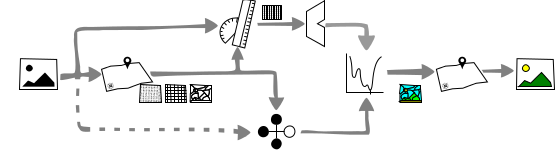
\includegraphics[width=0.9\linewidth]{method}
  \caption{Conceptual block representation of the segmentation methodology.}%\footnotemark}
    %\footnote{\cref{fig:methodTerms} illustrates the $\mathcal{S}$, $D(\cdot)$, and $V(\cdot)$ for the applied case of delineating breast structures in \ac{us} data.}
    %\footnote{(todo:add all the names of the elements in the figure)}
  \label{fig:method}
\end{figure}


To formulate segmentation as a metric labelling problem, the image is conceived as a discrete set of elements $\mathcal{S}$ that need to be labelled using a label $l$ from the labelling set $\mathcal{L}$.
Let $\mathcal{W}$ be all the possible labelling configurations of the set $\mathcal{S}$, given $\mathcal{L}$.
Let $U(\cdot)$ be a cost function encoding the goodness of the labelling configuration $\omega \in \mathcal{W}$ based on the appearance of the elements in $\mathcal{S}$, their inner relation and some designing constraints.
Then, the desired segmentation $\hat{\omega}$ corresponds to the labelling configuration that minimizes this cost function, as described in Eq.\,\eqref{eq:costMin}.

\begin{equation}
\hat{\omega} = \arg \min_{\substack{\omega}} \,U(\omega)
\label{eq:costMin}
\end{equation}

% \footnotetext{\Cref{fig:methodTerms} illustrates the $\mathcal{S}$, $D(\cdot)$, and $V(\cdot)$ for the applied case of delineating breast structures in \ac{us} data.}

This goodness measure $U(\cdot)$ must be defined to take into account the appearance of the target region, its relation with other regions, and other designing constraints.
Equation~\eqref{eq:labelingeq} describes this cost function as the combination of two independent costs that need to be simultaneously minimized as a whole.

\begin{equation}
  U(\omega) = \sum_{s\in \mathcal{S}} D_s(\omega_s) + \sum_{s \in \mathcal{S}}\sum_{r \in \mathcal{N}_{s}} V_{s,r}(\omega_s,\omega_r)
  \label{eq:labelingeq}
\end{equation}

Where, the left-hand side of the expression integrates the so-called \emph{data} term, while the right-hand side integrates the \emph{pairwise} term, which is also referred to as the \emph{smoothing} term.
Both terms are shaped by $\mathcal{S}$ and evaluated in the labelling space $\mathcal{W}$.
%
In our quest to optimize the cost function $U(\cdot)$, it is required to define a representation for the set $\mathcal{S}$, a data term $D(\cdot)$, a pairwise term $V(\cdot)$, and a proper minimization methodology.

\paragraph{The set $\mathcal{S}$}
can be, in general, any discrete set representing the image (i.e.\, pixels, overlapping or non overlapping windows, super-pixels, etc.).

\paragraph{The data term $D(\cdot)$,} \label{sec:method:dataTerm}
given a label configuration $\omega \in \mathcal{W}$, penalizes the labelling of a particular image element or site ($\omega_s = l$) based on the data associated to $s$.
In this manner, $D_s(\omega_s=l_\cmark) << D_s(\omega_s=l_\xmark)$.
Figure~\ref{fig:methodTerms}b illustrates the data cost associated to some arbitrary labelling configurations to clarify the desired effect (or behaviour) of this data term.
Designing an obscure heuristic to comply with the desired behaviour of $D(\cdot)$ out of the box, is rather a complicated task.
Therefore, an easier and cleaner approach is to design this data term $D(\cdot)$ with the help of \ac{ml} because it provides a systematic process that is flexible enough to encode any desired behaviour based on a training stage.
This concept is in fact depicted in the upper row in Fig.\,\ref{fig:method}.
For each site $s \in \mathcal{S}$, features describing $s$ are designed. Then, different optional steps can be applied to this set of features: (i) features normalization, (ii) features selection or (iii) features extraction. Finally, the data term $D(\cdot)$ is encoded based on \ac{ml} classifiers, the features and a training step.
Thus, the data term $D(\cdot)$ can be seen as a distance or goodness measure reflecting the likelihood for $s$ to belong to class $l$.


\begin{figure*}[!htb]
    \centering
    \begin{subfloat}
        \centering
        \begin{tikzpicture}
          \node[inner sep=0, ] (breast) {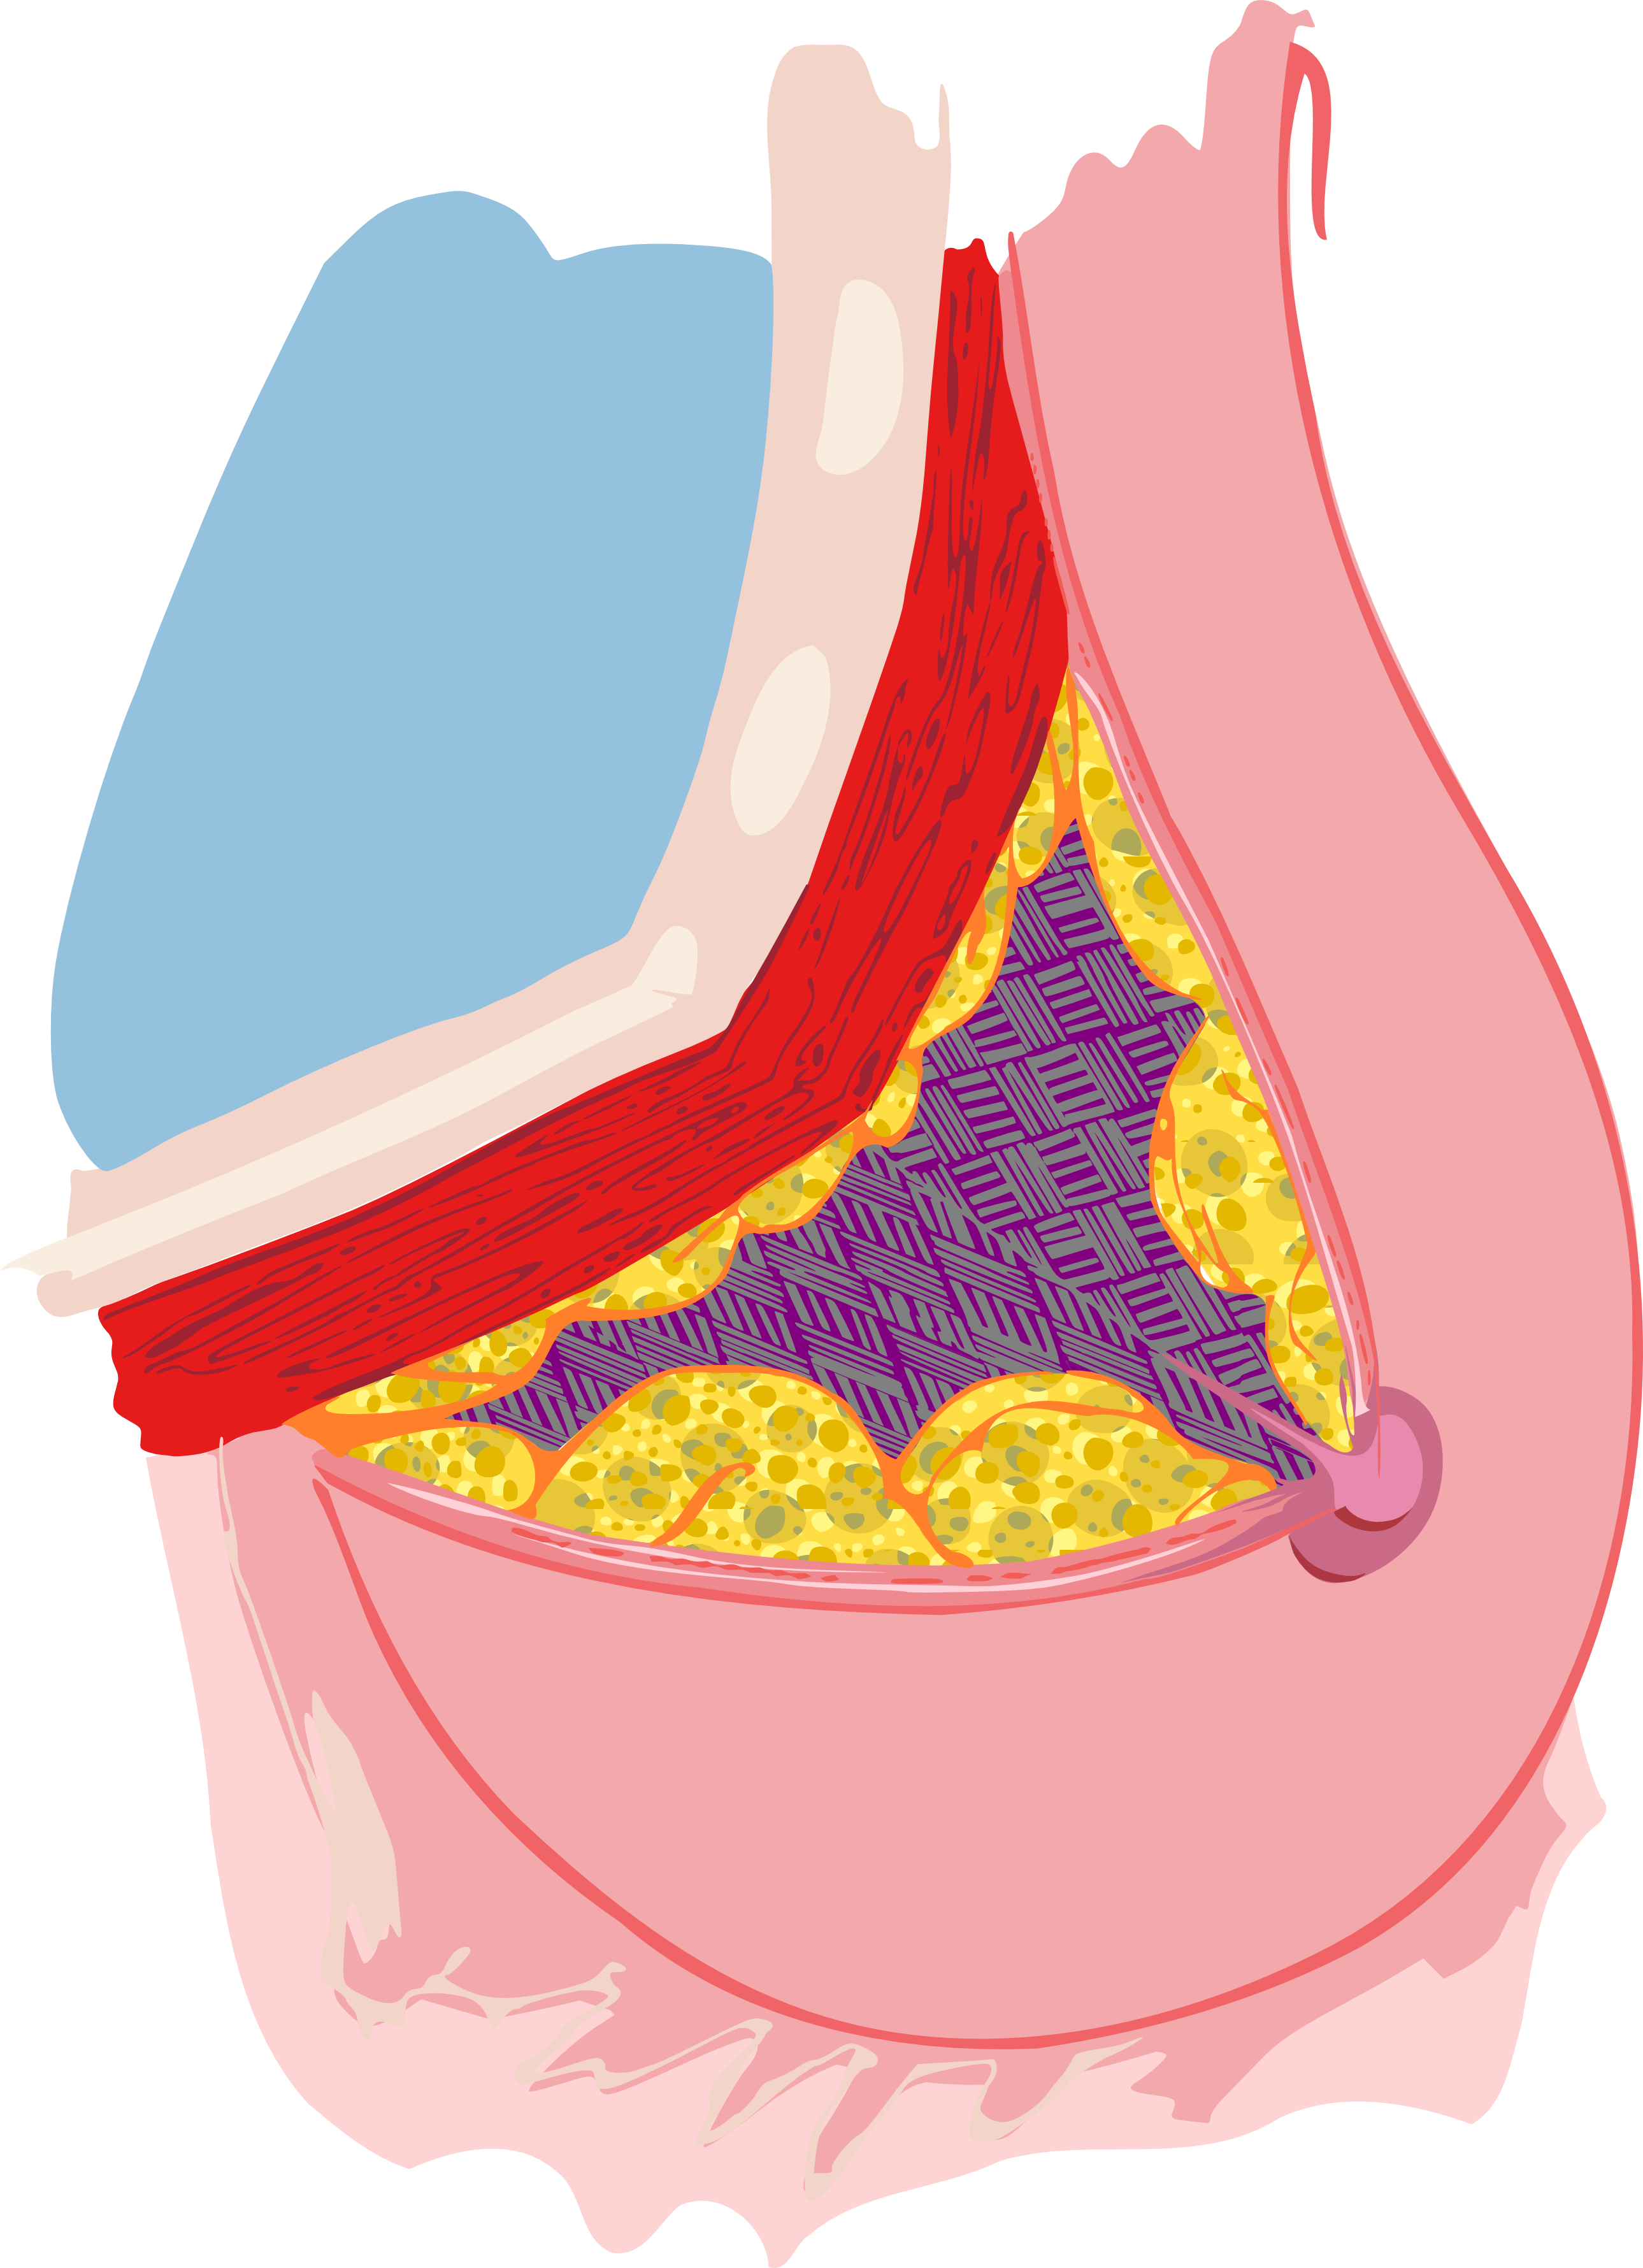
\includegraphics[width=0.1\textwidth]{breast}};
          \node[inner sep=0, below= 2pt of breast] (slice) {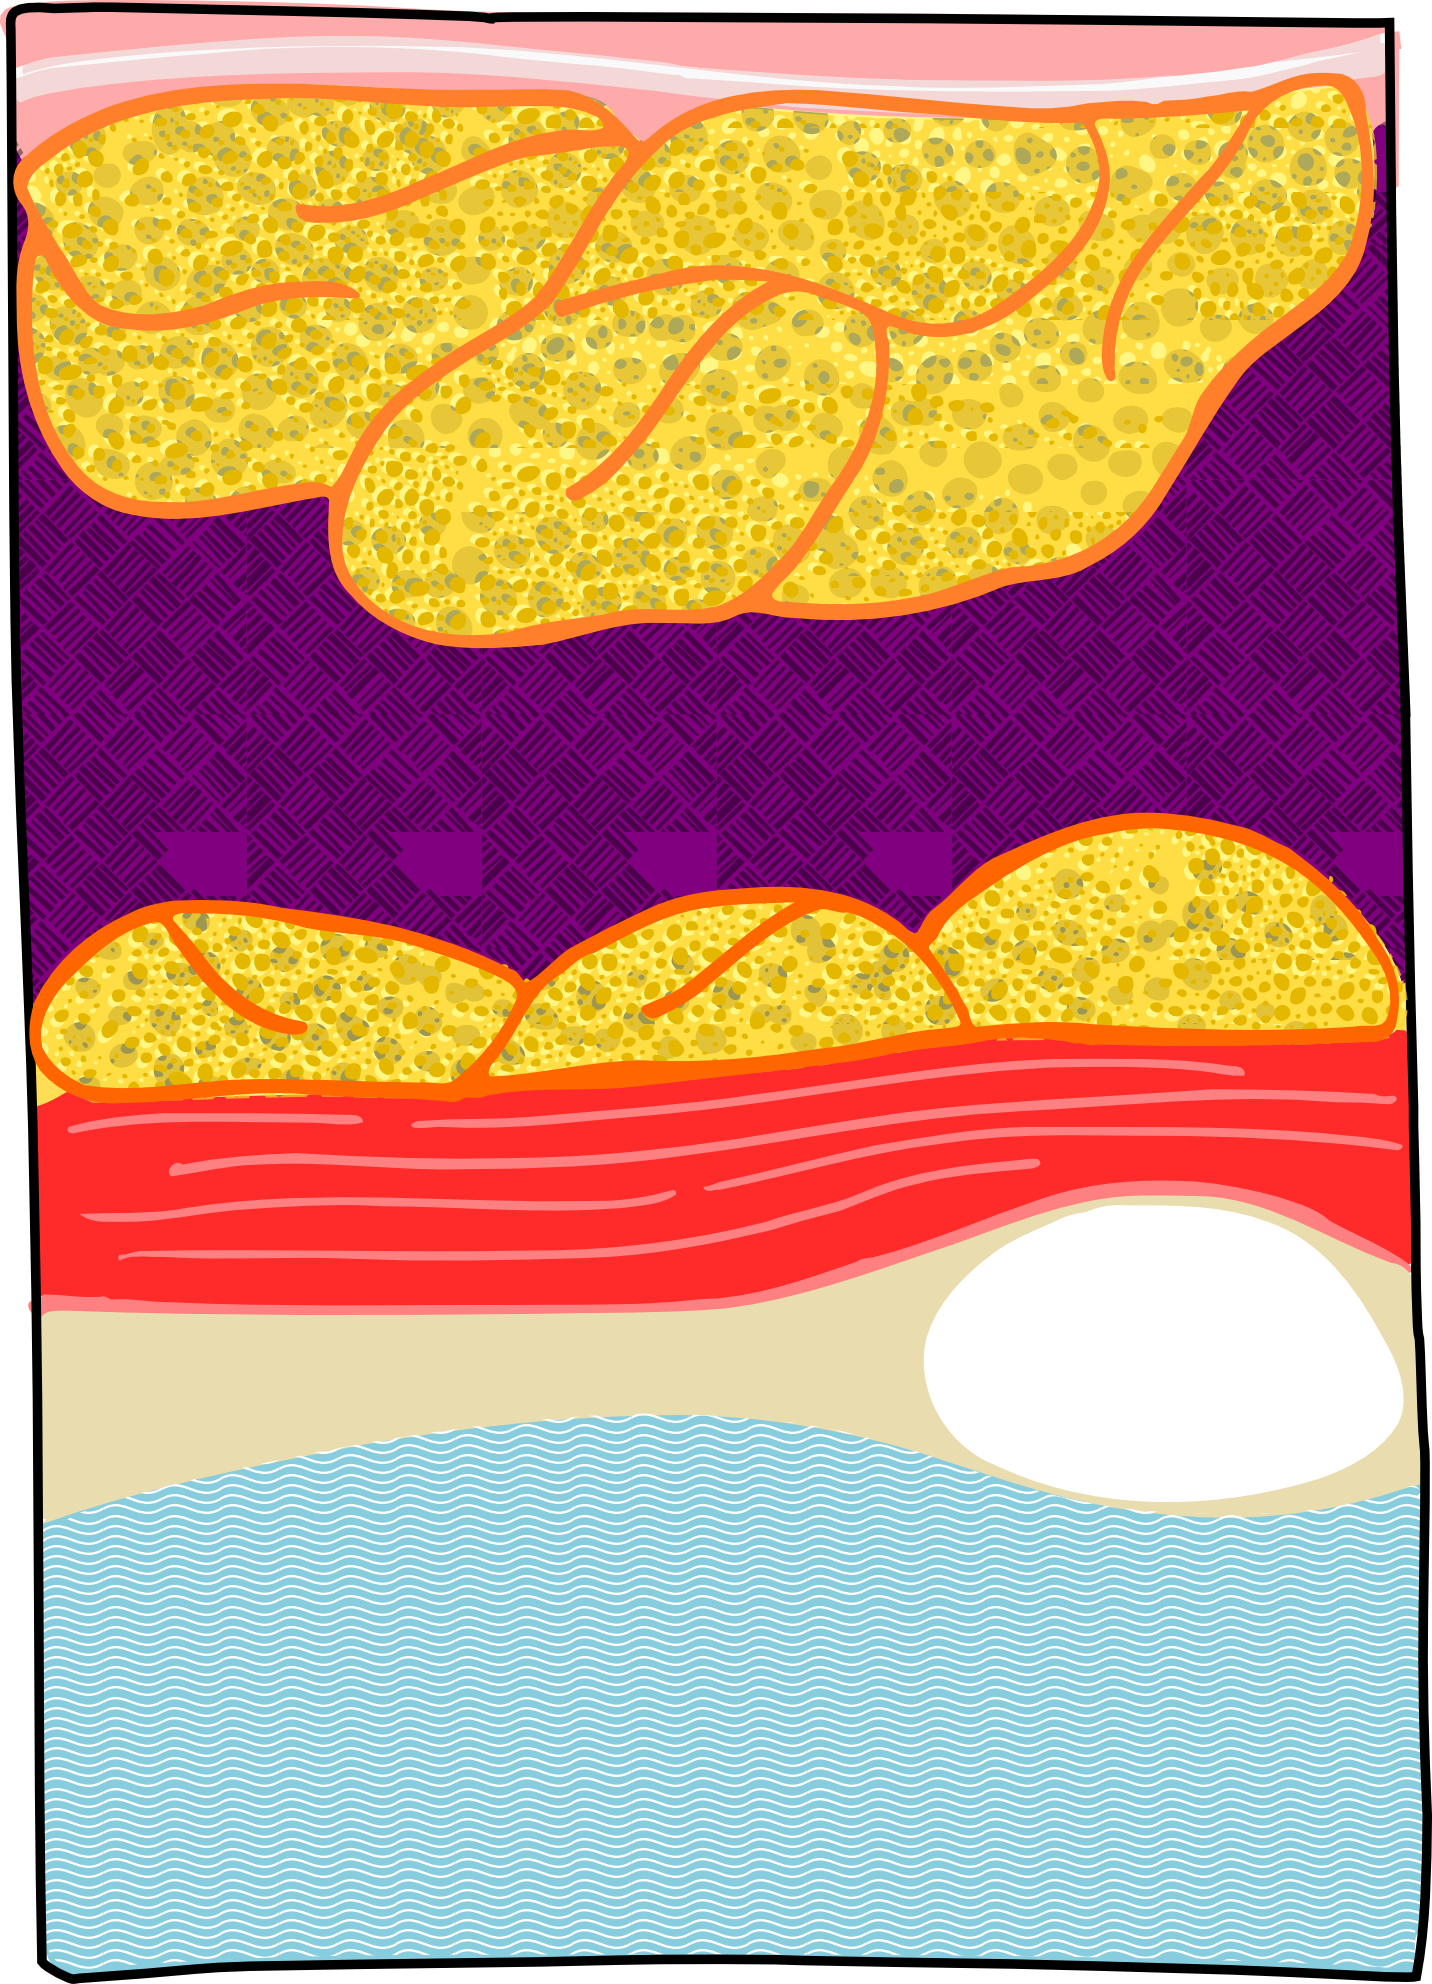
\includegraphics[width=0.1\textwidth]{slice}};
        \end{tikzpicture}
        %\caption{{\small Breast structure}}
        \label{fig:features:breast}
    \end{subfloat}
    ~~~
    %\hfill
    \begin{subfloat}
        \centering
        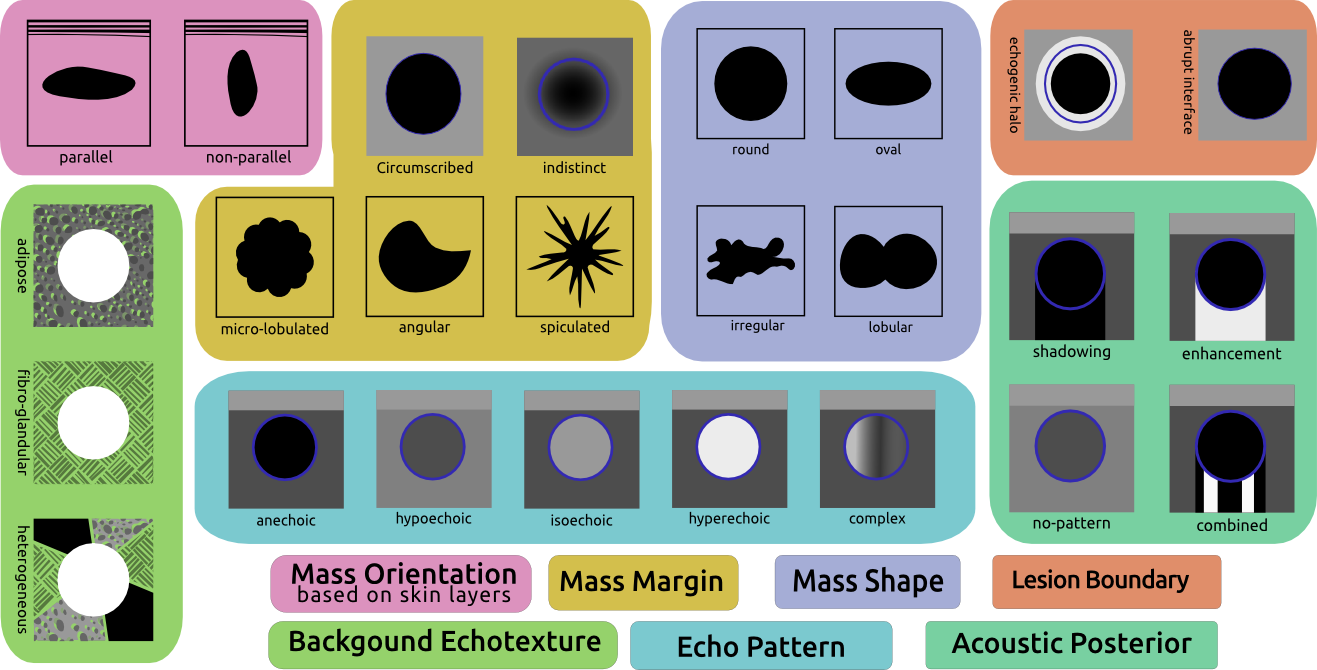
\includegraphics[width=.5\textwidth]{lexiconReworked}
        %\caption[]%
        %{Breast lesion characteristics in \ac{us} screening influencing clinical management~\cite{biradsus}}
        \label{fig:features:lexicon}
    \end{subfloat}
    %\hfill
    \caption {{\footnotesize Visual reference: (a) breast structures, (b) US BI-RADS lexicon}}
    \label{fig:features}
\end{figure*}

\paragraph{The pairwise term $V(\cdot,\cdot)$} \label{sec:method:mrfTerm}
%The pairwise term
represents the cost associated to $\omega_s$ taking into account the labels of its neighboring sites, $\omega_r$, $r \in \mathcal{N}_{s}$.
This term is usualy modeled using \ac{mrf} or \ac{crf}.
The typical form of this term, given in Eq.\,\eqref{eq:smoothing}, is called homogenization which acts as a regularization factor favouring configurations that have a coherent labelling.

\begin{equation}
V_{s,r}(\omega_s,\omega_r) =
\begin{cases}
    \beta, & \text{if } \omega_s \ne \omega_r\\
    0,              & \text{otherwise}
\end{cases}
\label{eq:smoothing}
\end{equation}

Figure~\ref{fig:methodTerms}c shows a visual interpretation of this cost.
The more fragmented is the segmentation $\omega$, the higher is the overall pairwise term, since every boundary brings a penalization $\beta$ to the total cost $U(\omega)$.
In this manner, the regularization term can be seen as a post-processing or denoising stage as some sites will flip their labelling if the cost of fragmenting the regions is larger than the cost of adopting their neighbour's label.

% Review %contribute have different or variable costs (see \cref{fig:methodTerms:boundary}) are also possible by taking into account not only relations in $\mathcal{S}$ of but also image information (see \cref{fig:method}).
%Further details can be found in \cref{sec:smoothing}.

\paragraph{The minimization strategy} \label{sec:method:min}
is determined by the nature of $U(\cdot)$ and $\mathcal{W}$, since not all the minimization strategies are applicable or adequate to find $\hat{\omega}$.
The size of the labelling space $|\mathcal{W}|=|\mathcal{L}|^{|\mathcal{S}|}$, discontinuities in $U(\omega)$ along $\mathcal{W}$ or the problem of local minima,
additionally all the particular of all the different minimization.
Need to be taken into account while choosing the most desirable minimization strategy.

%%% Local Variables:
%%% mode: latex
%%% TeX-master: "../../master.tex"
